\documentclass[a4paper,12pt]{article}
\usepackage{natbib}
\usepackage[margin=2.5cm]{geometry}
\usepackage{epsfig}
\usepackage{lscape}
\usepackage{setspace}
\usepackage{placeins}
\usepackage{floatrow}
\floatsetup[table]{capposition=top}
\floatsetup[figure]{capposition=top}
\usepackage{url}
\usepackage[utf8]{inputenc}
\usepackage[T1]{fontenc}
\usepackage{wrapfig}
\usepackage{comment}
\usepackage{amsmath,amsfonts,amssymb,amsthm}
\usepackage{bbm}
\usepackage{bm}
\usepackage{graphicx}
\usepackage{longtable}
\usepackage{ltxtable}
\usepackage{threeparttable}
\usepackage{booktabs}
\usepackage{multirow}
\usepackage{soul}
\usepackage{subcaption}
\usepackage{mathrsfs}
\usepackage[official]{eurosym}
\usepackage[usenames,dvipsnames,table]{xcolor}
\usepackage{circledsteps}
\usepackage{multicol}
\usepackage{amsthm}


\usepackage{hyperref}
\definecolor{red1}{RGB}{206, 17, 38}
\definecolor{blue1}{RGB}{16, 118, 208}
\definecolor{lightblue}{rgb}{0.8,0.85,1}
\newcommand{\red}[1]{\textcolor{red}{#1}}
\newcommand{\blue}[1]{\textcolor{blue}{#1}}
\newcommand{\green}[1]{\textcolor{emeraldgreen}{#1}}
\definecolor{bblue}{HTML}{377EB8}
\definecolor{bpink}{RGB}{219,32,101}
\definecolor{bth}{RGB}{13,17,55}
\newtheorem{proposition}{Proposition}
\newtheorem{assumption}{Definition}
\usepackage{ulem}

\newcommand{\strikethrough}[1]{
    \green{\sout{#1}}
}

\newif\ifcomment % define ifcomment
% --- Turn comments/markups on/off --------------
\commenttrue  % turn on comment/markups
%\commentfalse % turn off comment/markups
% -----------------------------------------------

% Define figure footer
\newcommand{\figurefooter}[1]{\floatfoot{
        {\setstretch{1.0}
            {\textsc{Note:} #1}
        }
    }
}

% Define threepart table settings
\usepackage{etoolbox}
\appto\TPTnoteSettings{}
\hypersetup{
    bookmarks=false,
    unicode=false,
    pdftoolbar=false,
    pdffitwindow=true,
    pdftitle={Econometricks: Short Guides to Econometrics},
    pdfauthor={Davud Rostam-Afschar},
    pdfsubject={Econometrics},
    pdfkeywords={Econometrics, Ordinary Least Squares, Maximum Likelihood, Generalized Method of Moments, Probability Theory, Distribution Theory, Frisch-Waugh-Lovell, Monte Carlo Simulation},
    pdfnewwindow=true,
    colorlinks=true,       % false: boxed links; true: colored links
    linkcolor=Blue,          % color of internal links (change box color with linkbordercolor)
    citecolor=Blue,        % color of links to bibliography
    filecolor=magenta,      % color of file links
    urlcolor=Blue,           % color of external links
	  pdfpagemode = UseNone,
	  plainpages=false,
}
\usepackage[hyperpageref]{backref}
\usepackage{tikz}
\bibliographystyle{econometrica}
\setlength{\bibsep}{0pt plus 0.3ex}

% Define URL and page style
\def\UrlBreaks{\do\/\do-}
\def\sym#1{\ifmmode^{#1}\else$^{#1}$\fi}
\pagestyle{plain}
% 1,5 -facher Zeilenabstand (Standard ist 1,2-facher Zeilenabstand, also 1,2*1,25 = 1,5
\renewcommand{\baselinestretch}{1.25}
% 1,5 -facher Zeilenabstand auch für die Tabellen
\renewcommand{\arraystretch}{1,25}
   \renewcommand*{\backref}[1]{}
   \renewcommand*{\backrefalt}[4]{
      \ifcase #1
         %Not cited.
      \or
         Cited on page~#2.
      \else
         Cited on pages~#2.
      \fi}
\onehalfspacing


% Define box and box title styles
\tikzstyle{mybox} = [draw=blue1, fill=blue1!5, very thick,
rectangle, rounded corners, inner sep=10pt, inner ysep=20pt]
\tikzstyle{dbox} = [draw=bpink, fill=bpink!1, very thick,
rectangle, rounded corners, inner sep=10pt, inner ysep=20pt]
\tikzstyle{thbox} = [draw=bth, fill=bth!10, very thick,
rectangle, rounded corners, inner sep=10pt, inner ysep=20pt]

% Redefine the comment box command to accept title and content

\newcommand{\bbox}[1]{
	\noindent\begin{tikzpicture}
		\node [mybox] (box) {
			\begin{minipage}{\textwidth}
				#1
			\end{minipage}
		};
	\end{tikzpicture}
}

\newcommand{\examplebox}[2]{
	\noindent\begin{tikzpicture}
		\node [mybox] (box) {
			\begin{minipage}{\textwidth}
				#2
			\end{minipage}
		};
		\node [etitle, right=10pt] at (box.north west) {#1};
	\end{tikzpicture}
}

\newcommand{\thbox}[2]{
	\begin{tikzpicture}
		\node [thbox] (box) {
			\begin{minipage}{\textwidth}
				#2
			\end{minipage}
		};
		\node [thtitle, right=10pt] at (box.north west) {#1};
	\end{tikzpicture}
}

\tikzstyle{thstyle} = [draw=bth, fill=bth!10, very thick,
rectangle, rounded corners, inner sep=10pt, inner ysep=20pt]
\tikzstyle{responsestyle} = [rectangle, inner sep=10pt, inner ysep=10pt]
\tikzstyle{thtitle} =[fill=bth, text=white]

% Define box and box title styles
\tikzstyle{examplestyle} = [draw=blue1, fill=blue1!5, very thick,
rectangle, rounded corners, inner sep=10pt, inner ysep=20pt]
\tikzstyle{responsestyle} = [rectangle, inner sep=10pt, inner ysep=10pt]
\tikzstyle{etitle} =[fill=blue1, text=white]

\newcommand{\definitionbox}[2]{
	\noindent\begin{tikzpicture}
		\node [dbox] (box) {
			\begin{minipage}{\textwidth}
				#2
			\end{minipage}
		};
		\node [fancytitle, right=10pt] at (box.north west) {#1};
	\end{tikzpicture}
}


% Define box and box title styles
\tikzstyle{definitionstyle} = [draw=teal, fill=bpink!5, very thick,
rectangle, rounded corners, inner sep=10pt, inner ysep=20pt]
\tikzstyle{responsestyle} = [rectangle, inner sep=10pt, inner ysep=10pt]
\tikzstyle{fancytitle} =[fill=bpink, text=white]


\newtheorem{definition}{Definition}
\def\emph{\textit}
%--------------------------------------------------------------------------------------% Begin of Document %--------------------------------------------------------------------------------------%
\begin{document}
\pagebreak
\title{
\huge \hspace{-1pt}Econome\textcolor{red1}{tricks}: Short Guides to Econometrics\thanks{These guides were developed based on lectures delivered by Davud Rostam-Afschar at the University of Mannheim. I am grateful for the valuable input provided by numerous cohorts of PhD students at the Graduate School of Economic and Social Sciences, University of Mannheim. I thank the Deutsche Forschungsgemeinschaft (DFG, German Research Foundation) for financial support through CRC \textit{TRR 266 Accounting for Transparency} (Davud Rostam-Afschar, Project-ID 403041268). Replication files and updates are available \href{https://rostam-afschar.de/metricks/metricks.htm}{here}.}
\\}

\author{
\normalsize\begin{tabular}{c}
%--------Anonymize--------------------------
Davud Rostam-Afschar\footnote{University of Mannheim, 68131 Mannheim, Germany; GLO; IZA; NeST (e-mail: rostam-afschar@uni-mannheim.de),}\\
%--------Anonymize--------------------------
{\date{\begin{small}\today\end{small}\\
}
}
\end{tabular}
}
%-------------------------------------------
\maketitle

\begin{abstract}
\noindent  Short guides to econometrics illustrate statistical methods and demonstrate how they work in theory and practice. With many examples.\\[2ex]

\noindent\textbf{Keywords:} Econometrics, Ordinary Least Squares, Maximum Likelihood, Generalized Method of Moments, Probability Theory, Distribution Theory, Frisch-Waugh-Lovell, Monte Carlo Simulation\\
\noindent \textbf{JEL classification:} A20, A23, C01, C10, C12, C13
\vfill
\end{abstract}

\newpage
	\tableofcontents
\newpage
%--------------------------------------------------------------------------------------% Introduction %--------------------------------------------------------------------------------------%
\section{Review of Probability Theory}
\subsection{Introduction}
\label{sec: Introduction}
This guide takes a look under the hood of widely used methods in econometrics and beyond. It focuses on Ordinary Least Squares, Maximum Likelihood, Generalized Method of Moments. It shows when and why these methods work with simple examples. This guide also provides an overview of the most important fundamentals of Probability Theory and Distribution Theory on which these methods are based and how to analyze them with the Frisch-Waugh-Lovell decomposition and with Monte Carlo Simulation.

\subsection{Probability fundamentals}
\label{sec: Probability fundamentals}
\subsubsection*{Discrete and continuous random variables}

\definitionbox{Discrete Random Variable}{
   \begin{minipage}{.49\linewidth}


   A random variable $X$ is \textbf{discrete} if the set of outcomes $x$ is either finite or countably infinite.
   \end{minipage}
    \begin{minipage}{.49\linewidth}
\hfill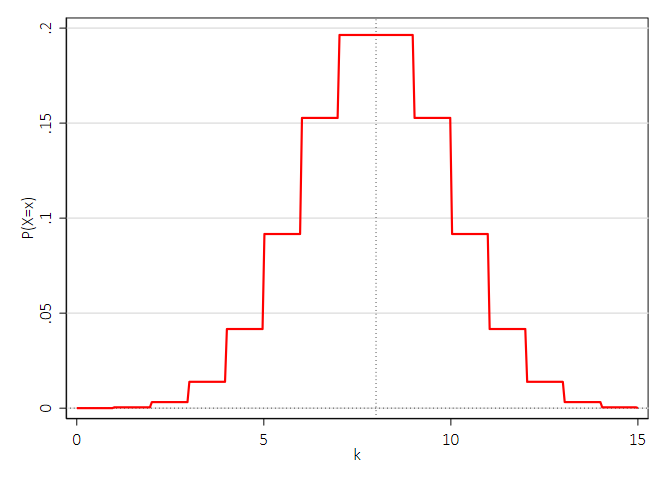
\includegraphics[width=.9\linewidth]{figures/binomial_pdf}
\end{minipage}
}

\definitionbox{Continuous Random Variable}{
   \begin{minipage}{.49\linewidth}
   The random variable $X$ is $\textbf{continuous}$ if the set of outcomes $x$ is infinitely divisible and, hence,
not countable.
   \end{minipage}
    \begin{minipage}{.49\linewidth}
\hfill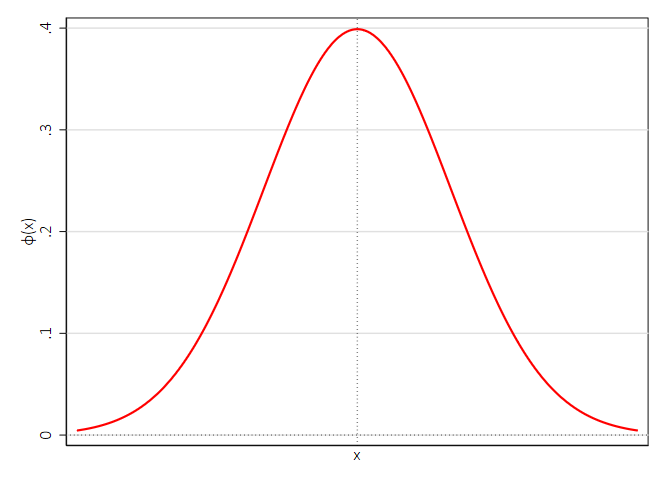
\includegraphics[width=.9\linewidth]{figures/normal_pdf}
\end{minipage}
}



\subsubsection*{Discrete probabilities}
For values $x$ of a discrete random variable $X$, the \textbf{probability mass function} (pmf)
$$f(x)=Prob(X=x).$$
The axioms of probability require
$$0\leq Prob(X=x)\leq1,$$
$$\sum_x f(x)=1.$$


\subsubsection*{Discrete cumulative probabilities}
For values $x$ of a discrete random variable $X$, the \textbf{cumulative distribution function}
$$F(x)=\sum_{X\leq x}f(x)=Prob(X\leq x),$$
where
$$f(x_i)=F(x_i)-F(x_{i-1}).$$
\examplebox{Example}{


Roll of a six-sided die



	\begin{center}
		\begin{threeparttable}[htbp]

\label{tab:timeline}

		\begin{tabular}{lll}
\toprule
$x$ & $f(x)$ & $F(X\leq x)$\\
\midrule
1 & $f(1)=1/6$ & $F(X\leq 1)=1/6$\\
2 & $f(2)=1/6$ & $F(X\leq 2)=2/6$\\
3 & $f(3)=1/6$ & $F(X\leq 3)=3/6$\\
4 & $f(4)=1/6$ & $F(X\leq 4)=4/6$\\
5 & $f(5)=1/6$ & $F(X\leq 5)=5/6$\\
6 & $f(6)=1/6$ & $F(X\leq 6)=6/6$\\
\bottomrule
		\end{tabular}

	\end{threeparttable}
\end{center}

%-------------------------------------------
What's the probability that you roll a 5 or higher?

$F(X\geq 5) = 1 - F(X\leq 4) = 1-2/3 = 1/3.$
}



\subsubsection*{Continuous probabilities}
For values $x$ of a continuous random variable $X$, the probability is zero but the area under $f(x)\geq0$ in the range form $a$ to $b$ is the \textbf{probability density function} (pdf)
$$Prob(a\leq x\leq b)=Prob(a< x< b)=\int_a^bf(x)dx\geq 0.$$
The axioms of probability require
$$\int^{+\infty}_{-\infty} f(x)dx=1.$$
$f(x)=0$ outside the range of $x$.\\
The \textbf{cumulative distribution function} (cdf) is
$$F(x)=\int_{-\infty}^x f(t)dt,$$
$$f(x)=\frac{dF(x)}{dx}.$$


\subsubsection*{Cumulative distribution function}
For continuous and discrete variables, $F(x)$ satisfies

\definitionbox{Properties of cdf}{
\begin{itemize}
	\item $0\leq F(x)\leq 1$
	\item If $x>y$, then $F(x)\geq F(y)$
	\item $F(+\infty)=1$
	\item $F(-\infty)=0$
\end{itemize}
and $$Prob(a< x\leq b)=F(b)-F(a).$$
}




\subsubsection*{Symmetric distributions}
For symmetric distributions $$f(\mu - x) = f(\mu + x)$$
and $$1-F(x)=F(-x).$$
\begin{figure}[H]
\begin{center}
%\scalebox{.36}
{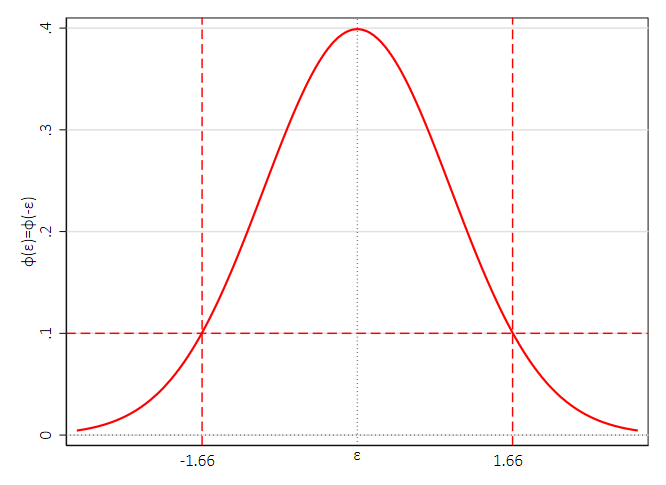
\includegraphics[width=0.49\textwidth]{figures/normal_pdf_sym}}\label{normal_pdf_sym}
{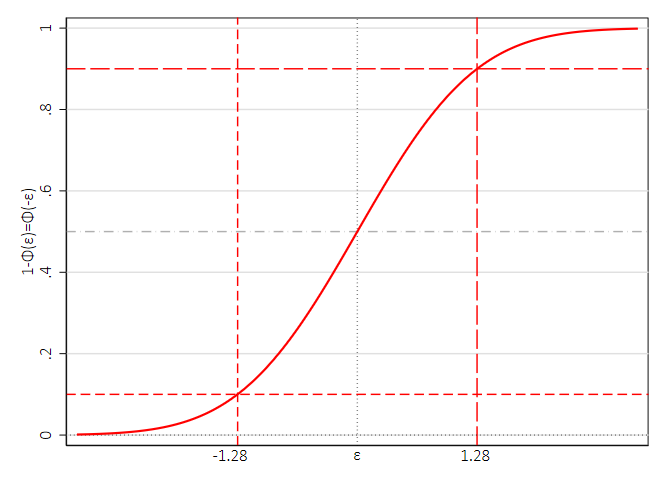
\includegraphics[width=0.49\textwidth]{figures/normal_cdf_sym}}\label{normal_cdf_sym}
\end{center}
\end{figure}


\subsection{Mean and variance}

\definitionbox{Mean of a random variable (Discrete)}{
The $\textbf{mean}$, or $\textbf{expected value}$, of a discrete random variable is
\begin{equation} \mu=E[x]=
\sum_{x}xf(x) \nonumber
\end{equation}
}
\examplebox{Example}{


Roll of a six-sided die


%-------------------------------------------

	\begin{center}
		\begin{threeparttable}[htbp]
\label{tab:timeline}

		\begin{tabular}{lll}
\toprule
$x$ & $f(x)=1/n$ & $F(X\leq x)=(x-a+1)/n$\\
\midrule
a = 1 & $f(1)=1/6$ & $F(X\leq 1)=1/6$\\
2 & $f(2)=1/6$ & $F(X\leq 2)=2/6$\\
3 & $f(3)=1/6$ & $F(X\leq 3)=3/6$\\
4 & $f(4)=1/6$ & $F(X\leq 4)=4/6$\\
5 & $f(5)=1/6$ & $F(X\leq 5)=5/6$\\
b = 6 & $f(6)=1/6$ & $F(X\leq 6)=6/6$\\
\bottomrule
		\end{tabular}
	\end{threeparttable}
\end{center}

%-------------------------------------------
What's the expected value from rolling the dice?

$E[x]=1/6+2/6+3/6+4/6+5/6+6/6=3.5.$

This is the mean (and the median) of a uniform distribution $(n+1)/2=(a+b)/2=3.5$.\\
}




\definitionbox{Mean of a random variable (Continuous)}{
For a continuous random variable $x$, the expected value is $$E[x]={\int_{x}xf(x)dx.}$$}

\examplebox{Example}{


The continuous uniform distribution is $1/(b-a)$ for $a\leq x\leq b$ and $0$ otherwise.\\

$$E[x]={\int_{a}^b\frac{x}{b-a}dx}={\frac{1}{b-a}\int_{a}^bxdx}.$$

Antiderivative of $x$ is $x^2/2$
$$E[x]={\frac{1}{b-a} (b^2/2-a^2/2)}=\frac{(b-a)(b+a)}{2(b-a)}=\frac{a+b}{2}.$$


The mean (and the median) is again $(a+b)/2=3.5$.
}

For a function $g(x)$ of $x$, the expected value is $E[g(x)]=\sum_{x}g(x) Prob(X = x)$ or $E[g(x)]=\int_{x}g(x)f(x)dx$. If $g(x) = a + bx$ for constants $a$ and $b$, then $E[a + bx] = a + bE[x]$.\\




\definitionbox{Variance of a random variable}{
The $\textbf{variance}$ of a random variable $\sigma^{2}>0$ is
\begin{equation}\label{eq0} \sigma^2=Var[x] = E[(x - \mu)^{2}]=\left\{
 \begin{array}{ll}
 {\sum_{x}(x - \mu)^{2}f(x)~~~~if~ x~ is~ discrete, } \\
 {~}\\
 {\int_{x}(x - \mu)^{2}f(x)dx~~if~ x~ is~ continuous.}
 \end{array}
 \right.\nonumber
\end{equation} }

\examplebox{Example}{
Roll of a six-sided die. What's the variance $V[x]$ from rolling the dice?\\
The probability of observing $x$, $Pr(X=x)=1/n$, is discretely uniformly distributed
$$E[x]=\frac{n+1}{2}; \; (E[x])^2=\frac{(n+1)^2}{4}.$$}

\bbox{
$$E[x^2]=\sum_xPr(X=x)=\frac{1}{n}\sum_{x=1}^nx^2=\frac{(n+1)(2n+1)}{6} \text{ due to the sequence sum of squares}.$$
$$V[x] = E[x^{2}] - (E[x])^2.$$
 $V[x]=\frac{(n+1)(2n+1)}{6}-\frac{(n+1)^2}{4}=\frac{n^2-1}{12}=(6^2-1)/12\approx2.92.$\\
}





\definitionbox{Chebychev inequality}{

For any random variable $x$ and any positive constant $k>1$,
$$\Pr(\mu - k\sigma < x < \mu + k\sigma) \geq 1-\frac{1}{k^{2}}.$$}

\textbf{Share outside $k$ standard deviations}.\\
If $x$ is normally distributed, the bound is $1-(2\Phi(k)-1)$.
\begin{figure}[H]
\begin{center}
%\scalebox{.36}
{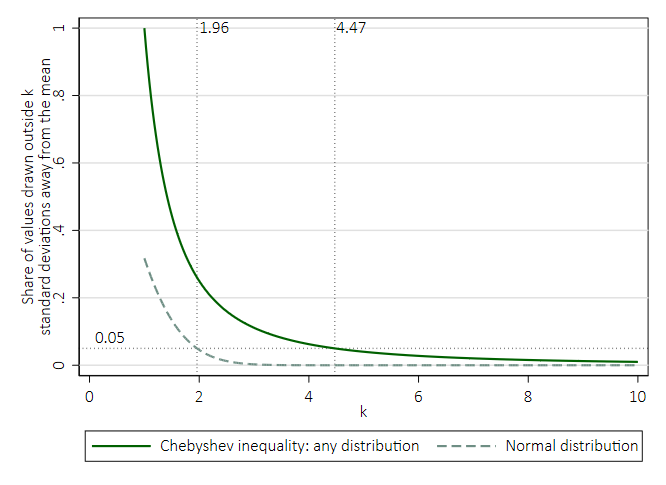
\includegraphics[width=0.9\textwidth]{figures/chebyshev_inequality_pdf}}\label{chebyshev_inequality_pdf}
\end{center}
\end{figure}
95\% of the observations are within 1.96 standard deviations for normally distributed $x$. If $x$ is not normal, 95\% are at most within 4.47 standard deviations.


\subsubsection*{Normal coverage}

\begin{figure}[H]
	\centering
		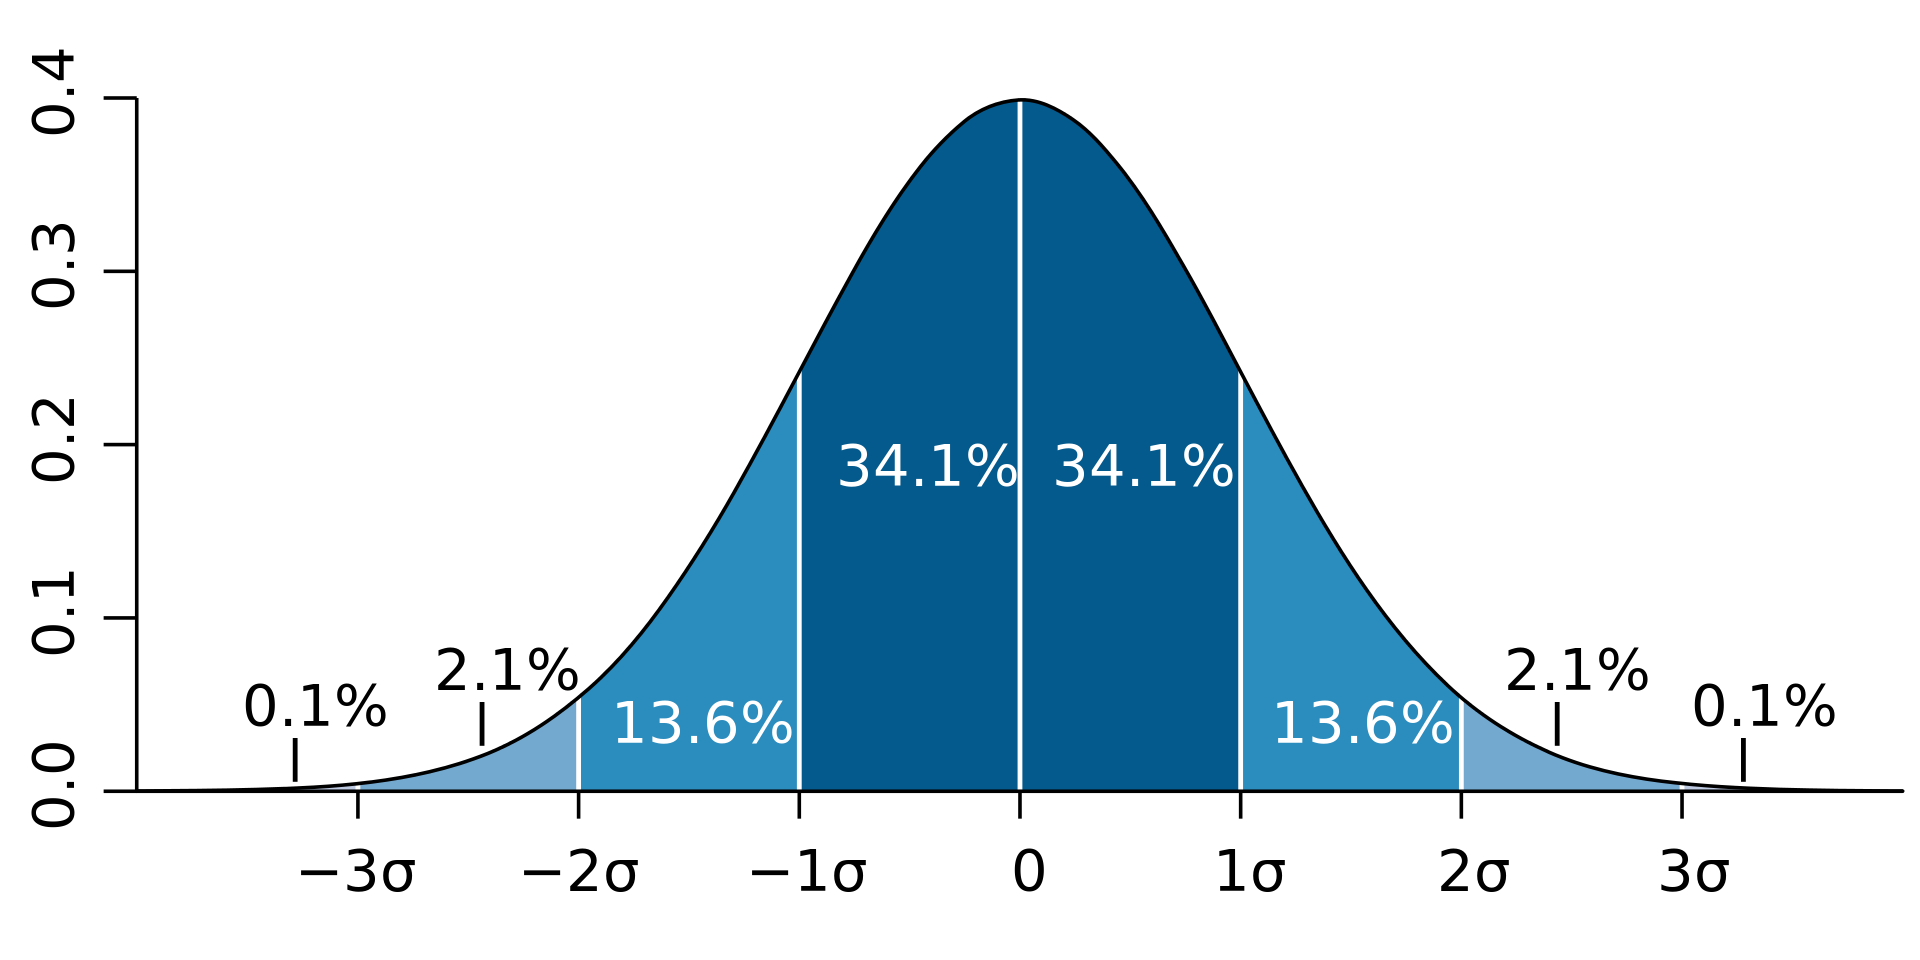
\includegraphics[width=0.90\textwidth]{figures/Standard_deviation_diagram}
	\label{fig:Standard_deviation_diagram}
\end{figure}



\subsection{Moments of a random variable}

\definitionbox{Central moments of a random variable}{
The central moments are
 \begin{equation*}
    \mu_{r} = E[(x - \mu)^{r}].
 \end{equation*}}

\examplebox{Example}{
\textbf{Moments:} Two measures often used to describe a probability distribution are
\begin{itemize}
	\item expectation $= E[(x - \mu)^{1}]$
	\item variance $= E[(x - \mu)^{2}]$
	\item skewness $= E[(x - \mu)^{3}]$
	\item kurtosis $= E[(x - \mu)^{4}]$
\end{itemize}
The skewness is zero for symmetric distributions.
}



\subsubsection*{Higher order moments}
\begin{figure}[H]
\begin{center}
{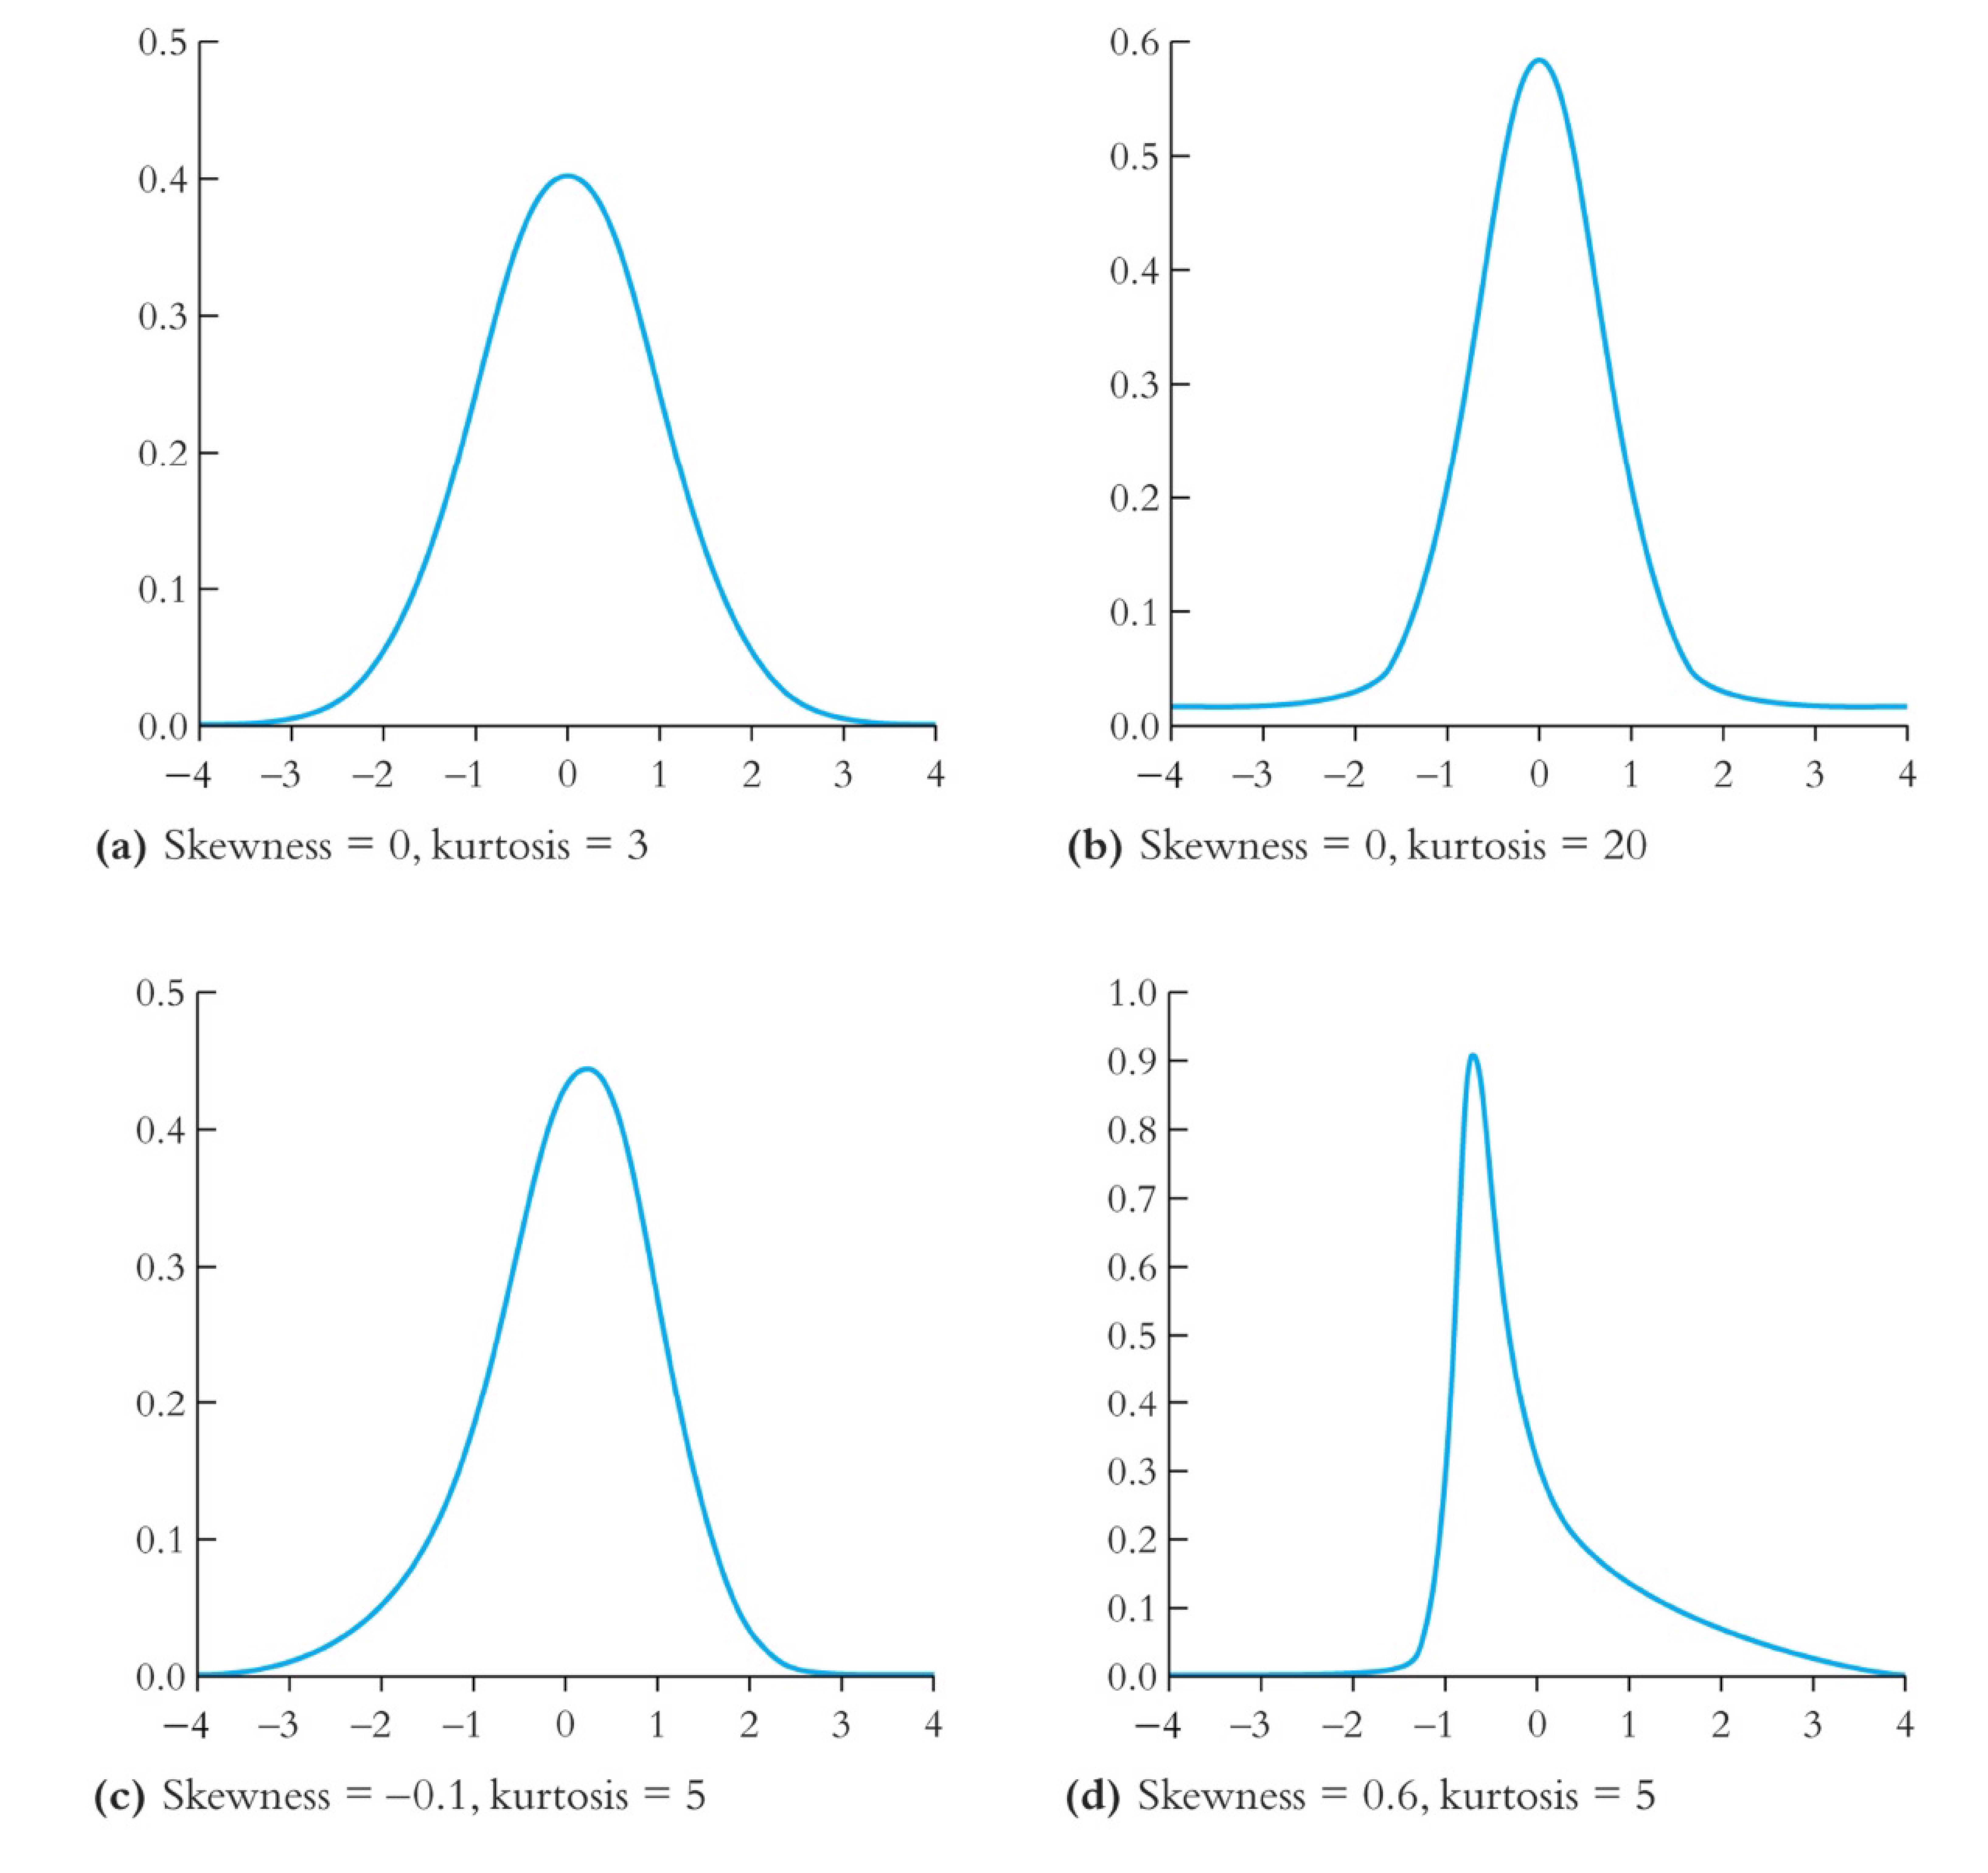
\includegraphics[width=0.9\textwidth]{figures/skewness_kurtosis}}\label{skewness_kurtosis}
\end{center}
\end{figure}


\definitionbox{Moment generating function}{
For the random variable $X$, with probability density function $f(x)$, if the function
\begin{equation*}
    M(t) = E[e^{tx}].
\end{equation*}
exists, then it is the $\textbf{moment generating function}(MGF)$.}

\begin{itemize}
	\item Often simpler alternative to working directly with probability density functions or cumulative distribution functions
	\item Not all random variables have moment-generating functions
\end{itemize}
The $n$th moment is the $n$th derivative of the moment-generating function, evaluated at $t=0$.\\

\examplebox{Example}{
The MGF for the standard normal distribution with $\mu=0, \sigma=1$ is $$M_{z}(t) = e^{\mu t+ \sigma^2t^{2}/2} = e^{t^{2}/2}.$$
If $x$ and $y$ are independent, then the MGF of $x + y$ is $M_{x}(t)M_{y}(t).$
}





For $x \sim N (\mu, \sigma^2)$ for some $\mu,\sigma>0$ with moment generating function

${M_x}(t) =  \exp (\mu t + \dfrac 1 2 \sigma^2 t^2)$, the first moment generating function of $x$ is
$$ E[(x - \mu)^{1}]={M_x}'(t)= (\mu +  \sigma^2 t)\exp \bigg(\mu t + \dfrac 1 2 \sigma^2 t^2\bigg).$$

\examplebox{Example}{
$$ E[(x - \mu)^{1}]={M_x}'(t) = \frac{d\bigg[\exp \bigg(\mu t + \dfrac 1 2 \sigma^2 t^2\bigg)\bigg]}{dt}$$
$$= \frac{d\bigg[\mu t + \dfrac 1 2 \sigma^2 t^2\bigg]}{dt}\frac{d\bigg[\exp \bigg(\mu t + \dfrac 1 2 \sigma^2 t^2\bigg)\bigg]}{d(\mu t + \dfrac 1 2 \sigma^2 t^2)}$$
$$ =(\mu +  \sigma^2 t)\exp \bigg(\mu t + \dfrac 1 2 \sigma^2 t^2\bigg).$$
}


If $x\sim N(0,1)$,
\begin{itemize}
	\item the skewness is $E[(x - \mu)^{3}]=0$ and
	\item the kurtosis is $E[(x - \mu)^{4}]=3$.
\end{itemize}

\examplebox{Example}{


$$E[(x - \mu)^{1}]={M_x}'(t) =(\mu +  \sigma^2 t)\exp \bigg(\mu t + \dfrac 1 2 \sigma^2 t^2\bigg) \text{ with } \mu=0, \sigma=1, t=0: E[x]=\mu=0$$
$$E[(x - \mu)^{2}]={M_x}''(t) =  \bigg(\sigma^2 + (\mu + \sigma^2 t)^2 \bigg)  \exp \bigg(\mu t + \dfrac 1 2 \sigma^2 t^2\bigg)$$ $$\text{ with } \mu=0, \sigma=1, t=0: E[(x - \mu)^{2}]=\sigma^2=1$$
$$E[(x - \mu)^{3}]={M_x}'''(t) =\bigg(3 \sigma^2 (\mu + \sigma^2 t) + (\mu + \sigma^2 t)^3\bigg)  \exp\bigg(\mu t + \dfrac 1 2 \sigma^2 t^2\bigg)$$
$$\text{with } \mu=0, \sigma=1, t=0: E[(x - \mu)^{3}]= 0$$
$$E[(x - \mu)^{4}]={M_x}^{(4)} (t) = \bigg(3 \sigma^4 + 6 \sigma^2 (\mu + \sigma^2 t)^2 + (\mu + \sigma^2 t)^4\bigg) \exp\bigg(\mu t + \dfrac 1 2 \sigma^2 t^2\bigg)$$
$$\text{with } \mu=0, \sigma=1, t=0: E[(x - \mu)^{4}]=3.$$
}


\subsubsection*{Approximating mean and variance}
For any two functions $g_{1}(x)$ and $g_{2}(x)$,
 \begin{equation}
    E[g_{1}(x) + g_{2}(x)] = E[g_{1}(x)] + E[g_{2}(x)].\nonumber
 \end{equation}
 For the general case of a possibly nonlinear $g(x)$,
 {\begin{equation}
    E[g(x)] =\int_{x}g(x)f(x)dx,\nonumber
 \end{equation}
 and
 \begin{equation}
    Var[g(x)] =\int_{x}\left(g(x) - E [g(x)]\right)^{2}f(x)dx.\nonumber
 \end{equation}}
$E[g(x)]$ and $Var[g(x)]$ can be approximated by a first order linear Taylor series:\\

\thbox{First order linear Taylor series}{
\begin{equation}\label{eq5}
    g(x)\approx [g(x^{0})-g^{\prime}(x^{0})x^{0}]+g^{\prime}(x^{0})x.
\end{equation}
}

\clearpage
\subsubsection*{Taylor approximation Order 1}
\begin{figure}[h!]
	\centering
		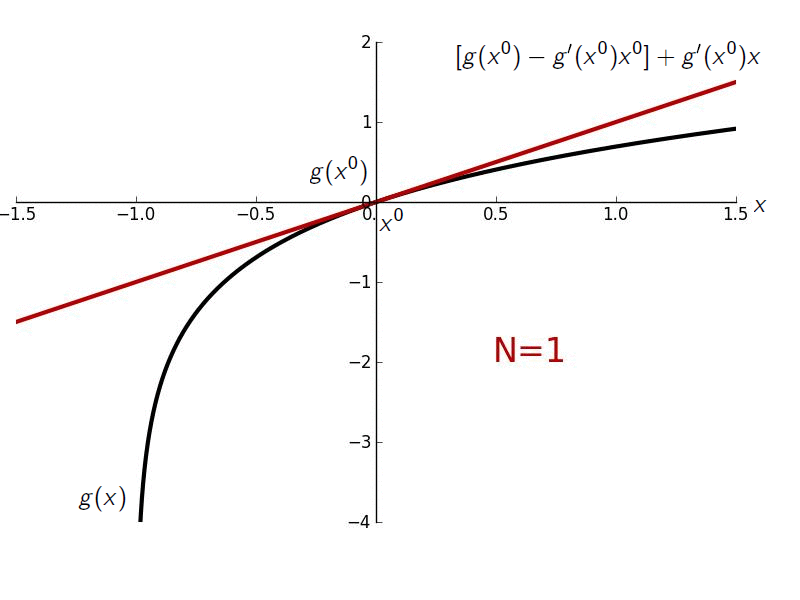
\includegraphics[width=0.90\textwidth]{figures/taylor1_formula}
	\label{fig:taylor1_formula}
\end{figure}
 

%
%\begin{paragraph}{Taylor approximation Order 1}
%\begin{figure}
	%\centering
		%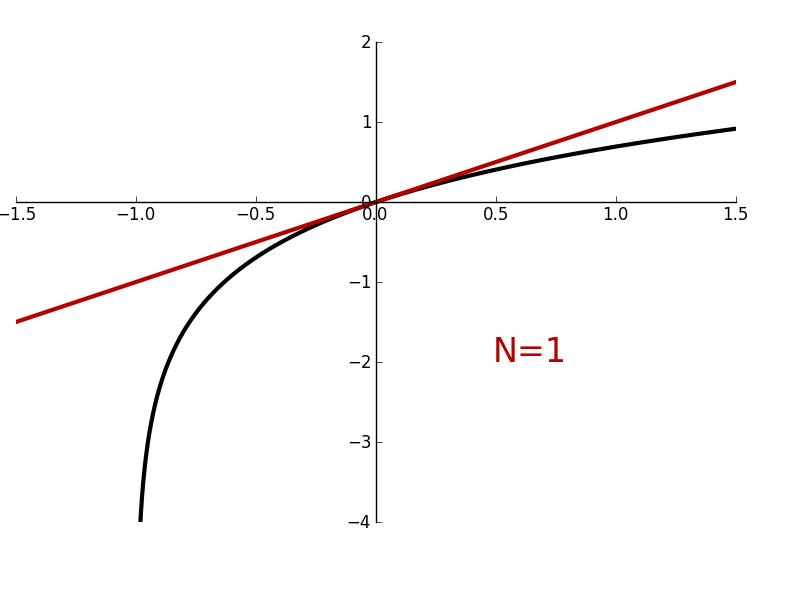
\includegraphics[width=0.90\textwidth]{taylor1.png}
	%\label{fig:taylor1}
%\end{figure}
%
%
%
%\begin{paragraph}{Taylor approximation Order 2}
%\begin{figure}
	%\centering
		%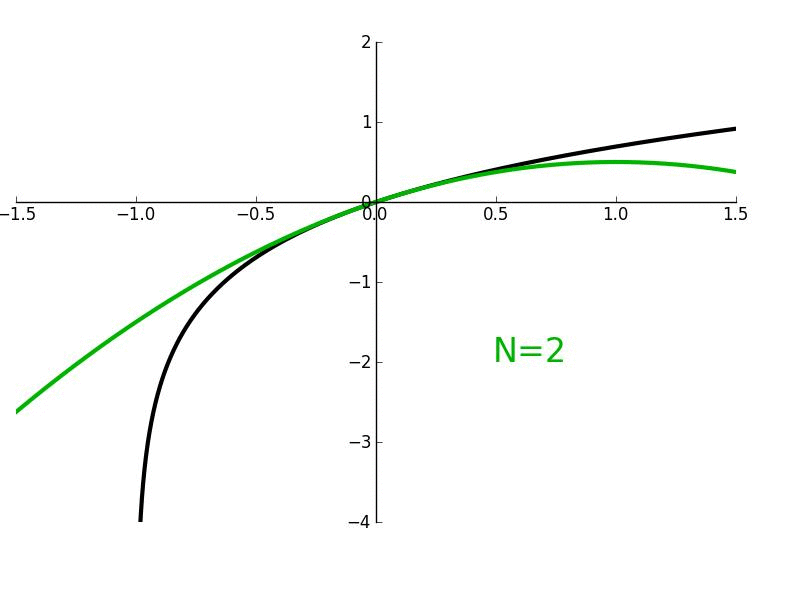
\includegraphics[width=0.90\textwidth]{taylor2.png}
	%\label{fig:taylor2}
%\end{figure}
%
%
%
%
%\begin{paragraph}{Taylor approximation Order 3}
%\begin{figure}
	%\centering
		%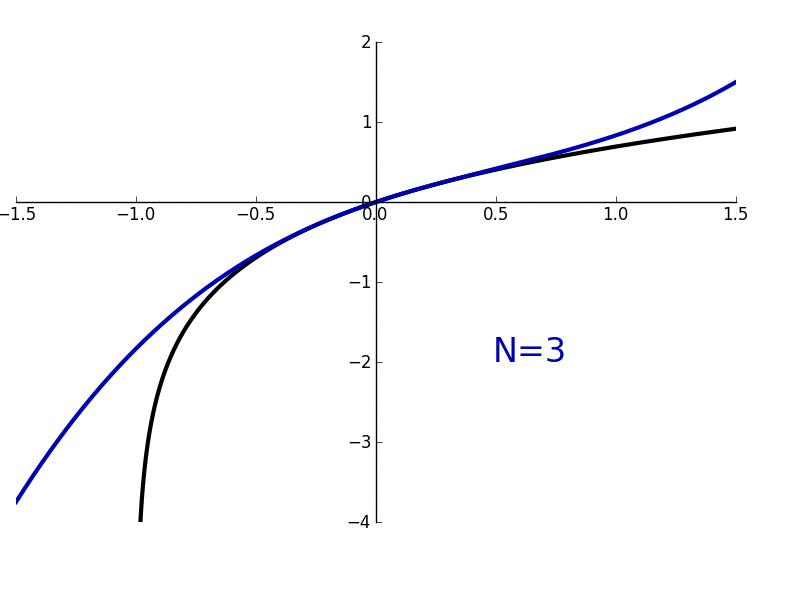
\includegraphics[width=0.90\textwidth]{taylor3.png}
	%\label{fig:taylor3}
%\end{figure}
%
%
%
%\begin{paragraph}{Taylor approximation Order 4}
%\begin{figure}
	%\centering
		%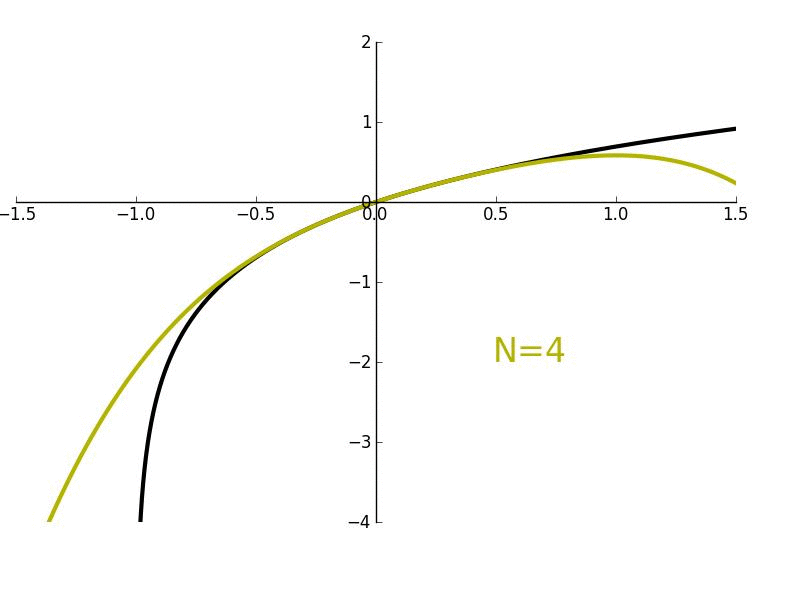
\includegraphics[width=0.90\textwidth]{taylor4.png}
	%\label{fig:taylor4}
%\end{figure}
%
%
%
%\begin{paragraph}{Taylor approximation Order 5}
%\begin{figure}
	%\centering
		%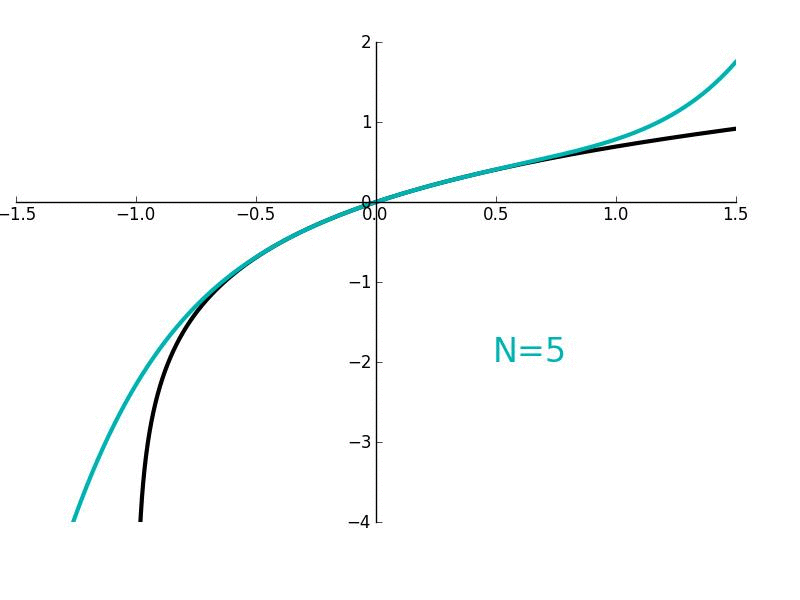
\includegraphics[width=0.90\textwidth]{taylor5.png}
	%\label{fig:taylor5}
%\end{figure}
%
%
%
%\begin{paragraph}{Taylor approximation Order 6}
%\begin{figure}
	%\centering
		%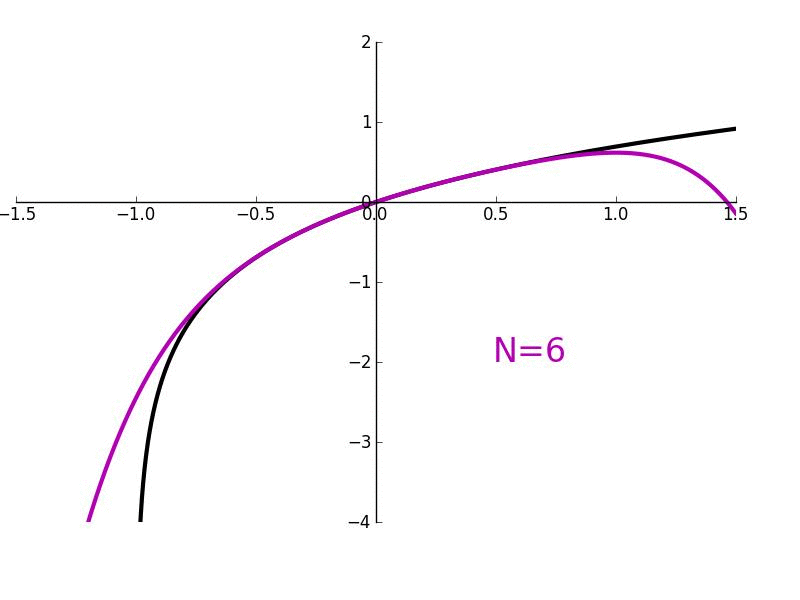
\includegraphics[width=0.90\textwidth]{taylor6.png}
	%\label{fig:taylor6}
%\end{figure}
%
%
%
%\begin{paragraph}{Taylor approximation Order 7}
%\begin{figure}
	%\centering
		%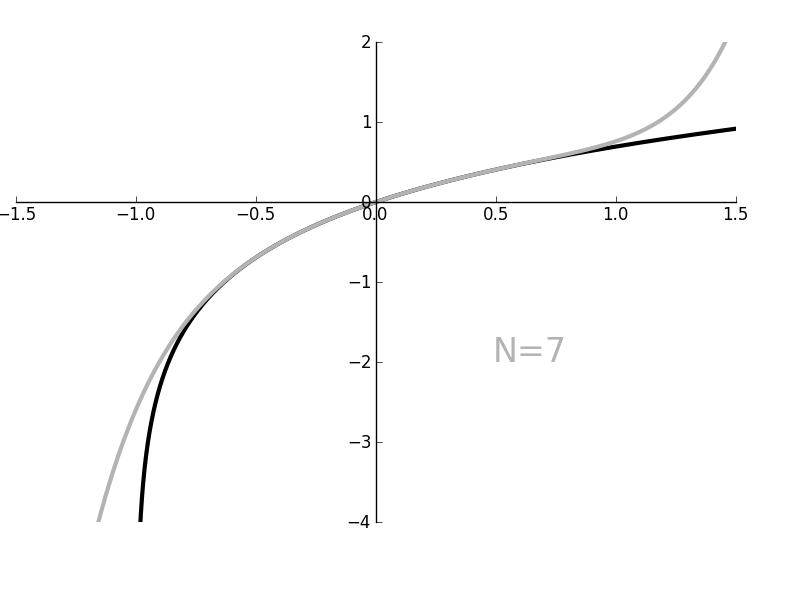
\includegraphics[width=0.90\textwidth]{taylor7.png}
	%\label{fig:taylor7}
%\end{figure}
%
%
%
%\begin{paragraph}{Taylor approximation Order 8}
%\begin{figure}
	%\centering
		%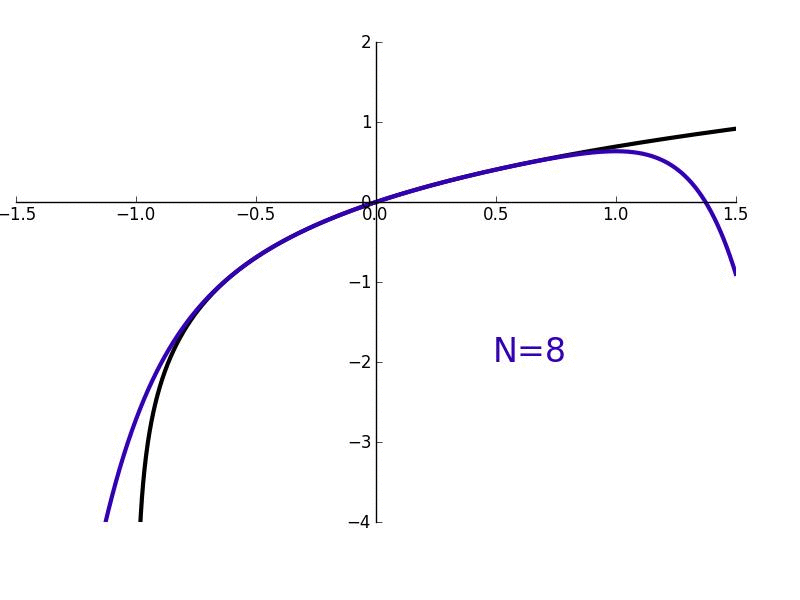
\includegraphics[width=0.90\textwidth]{taylor8.png}
	%\label{fig:taylor8}
%\end{figure}
%
%
%
%\begin{paragraph}{Taylor approximation Order 9}
%\begin{figure}
	%\centering
		%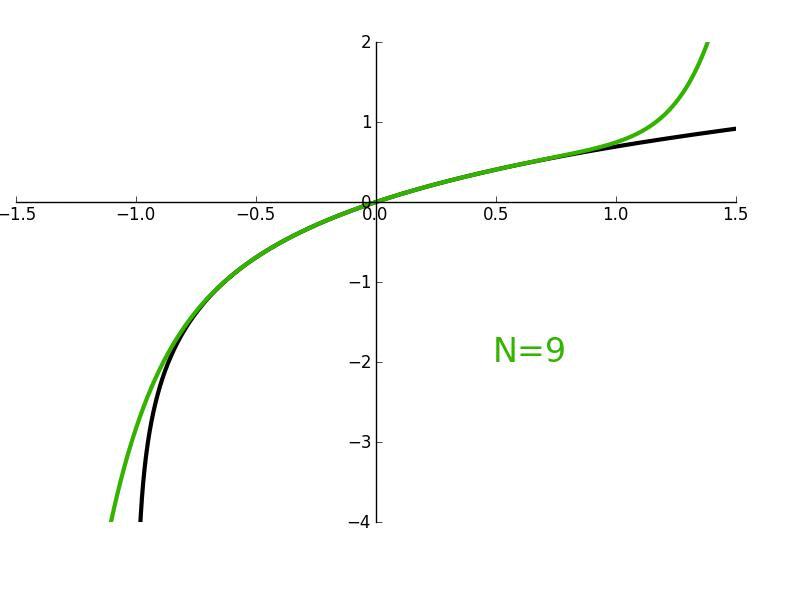
\includegraphics[width=0.90\textwidth]{taylor9.png}
	%\label{fig:taylor9}
%\end{figure}
%
%
%
%\begin{paragraph}{Taylor approximation Order 10}
%\begin{figure}
	%\centering
		%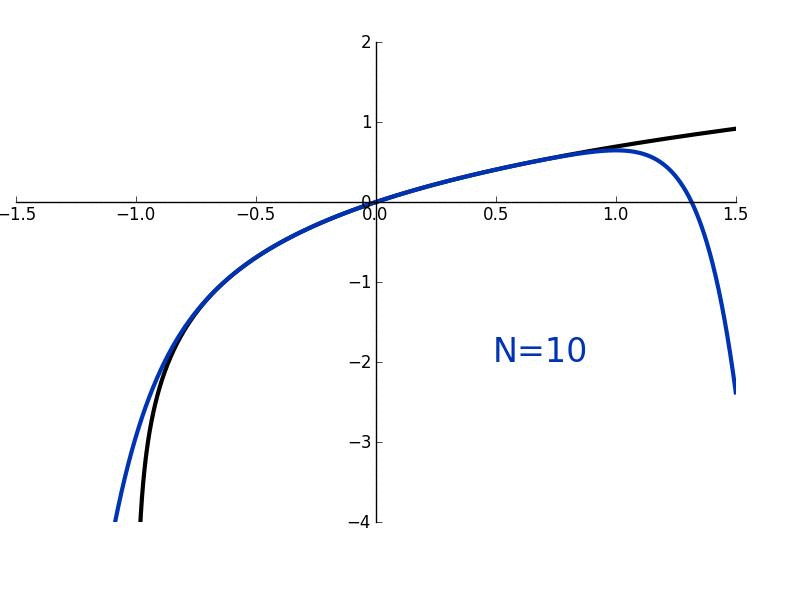
\includegraphics[width=0.90\textwidth]{taylor10.png}
	%\label{fig:taylor10}
%\end{figure}
%
%
%
%\begin{paragraph}{Taylor approximation Order 15}
%\begin{figure}
	%\centering
		%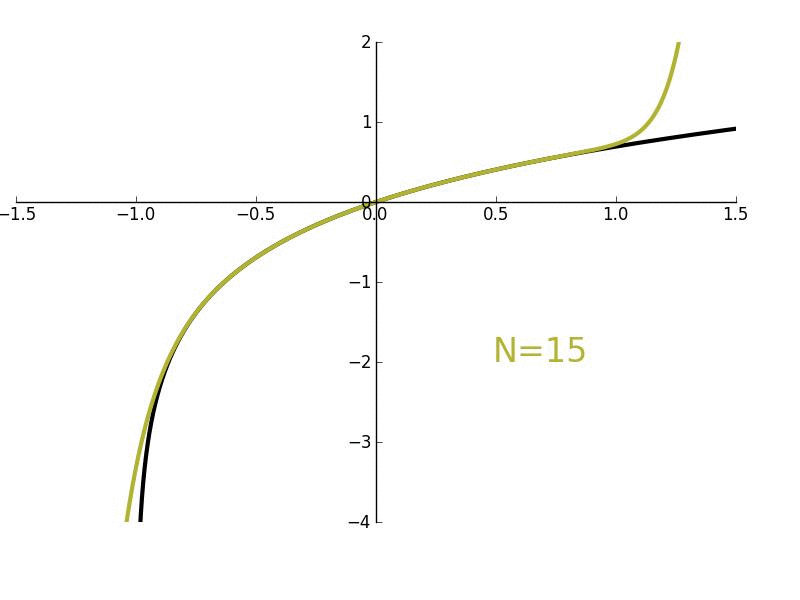
\includegraphics[width=0.90\textwidth]{taylor15.png}
	%\label{fig:taylor15}
%\end{figure}
%
%
%
%\begin{paragraph}{Taylor approximation Order 20}
%\begin{figure}
	%\centering
		%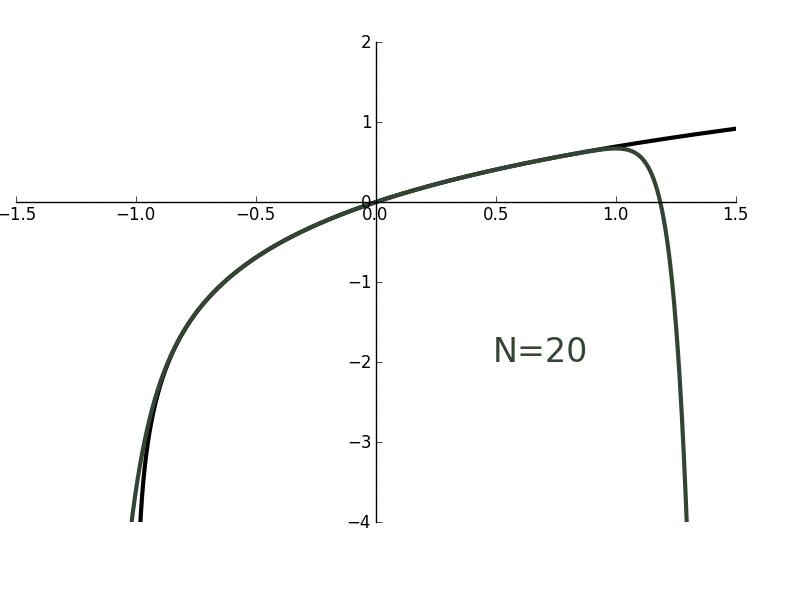
\includegraphics[width=0.90\textwidth]{taylor20.png}
	%\label{fig:taylor20}
%\end{figure}
%
%
%
%\begin{paragraph}{Taylor approximation Order 45}
%\begin{figure}
	%\centering
		%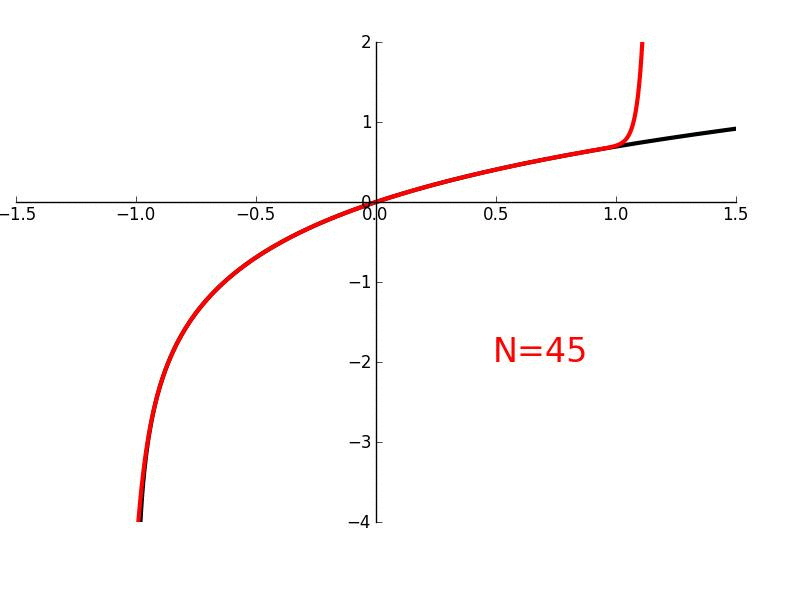
\includegraphics[width=0.90\textwidth]{taylor45.png}
	%\label{fig:taylor45}
%\end{figure}
%
%
%
%
%\begin{paragraph}{Taylor approximation Order 100}
%\begin{figure}
	%\centering
		%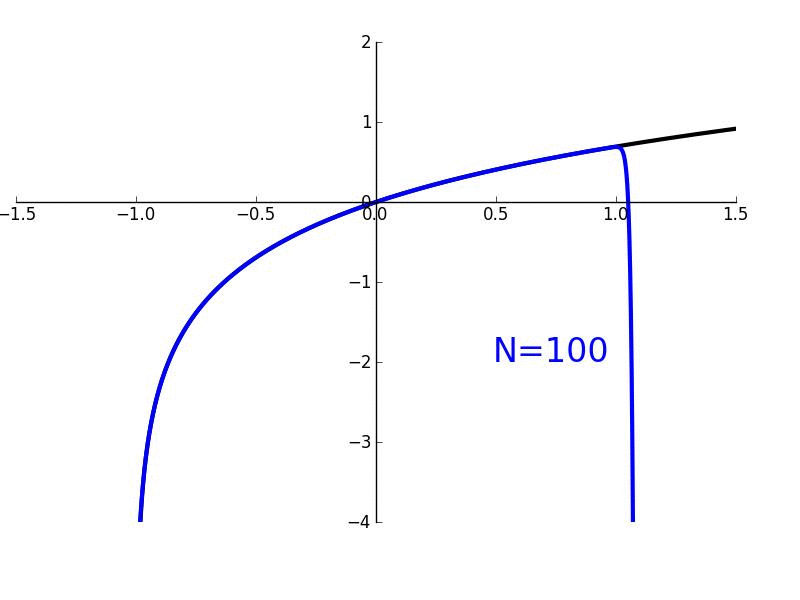
\includegraphics[width=0.90\textwidth]{taylor100.png}
	%\label{fig:taylor100}
%\end{figure}
%
%



A natural choice for the expansion point is $x^{0} = \mu = E(x)$. Inserting this value in Eq. (\ref{eq5}) gives
\begin{equation}\label{eq6}
    g(x)\approx [g(\mu)-g^{\prime}(\mu)\mu]+g^{\prime}(\mu)x,\nonumber
\end{equation}
so that
\begin{equation}\label{eq7}
    E[g(x)] \approx g(\mu),\nonumber
\end{equation}
and
\begin{equation}\label{eq8}
    Var[g(x)]\approx [g^{\prime}(\mu)]^{2} Var[x].\nonumber
\end{equation}\\

\examplebox{Example}{ \textbf{Isoelastic utility}.
$c_{bad}=$	10.00 Euro; $c_{good}=$	100.00 Euro;  probability good outcome	50\%\\[2ex]
$\mu=E[c]=1/2 \times c_{bad}+ 1/2 \times c_{good}=$55.00 Euro\\
$$u(c)= c^{1/2}$$
$u(\mu)= 7.42$ approximates $E[u(c)]= 1/2\times10^{1/2}+1/2\times100^{1/2}=6.58$
}








\examplebox{Example}{ \textbf{Isoelastic utility}.


$c_{bad}=$	10.00 Euro; $c_{good}=$	100.00 Euro;  probability good outcome	50\%; $\mu=55.00$ Euro\\[2ex]
\begin{minipage}{.4\textwidth}
$$u(c)= \ln(c)$$
$\begin{aligned}
u(\mu)&= 4.01 \text{ approx.}\\
E[u(c)]&= 1/2\times \ln(10)+1/2\times \ln(100)\\ &=3.45\end{aligned}$
\vskip 2em
\textbf{Jensen's inequality}:

$E[g(x)]\leq g(E[x])]$ if $g''(x)<0$.
\end{minipage}\hfill
\begin{minipage}{0.55\textwidth}

  \begin{center}
		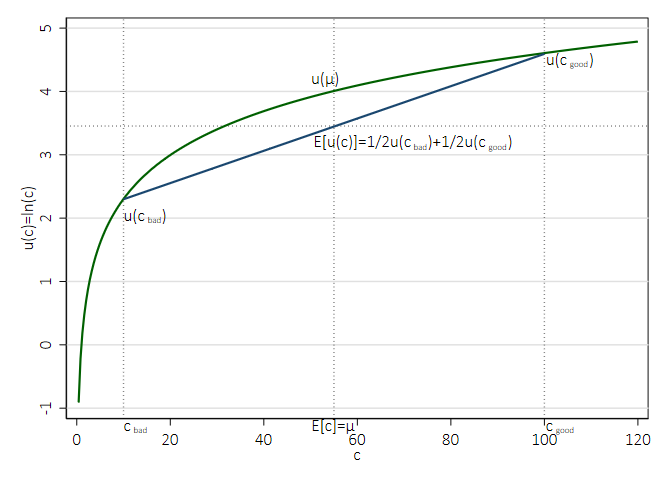
\includegraphics[width=\textwidth]{figures/Jensens_inequality}
	\label{fig:Jensens_inequality}
  \end{center}
\end{minipage}



$V[u(c)]\approx (1/55)^{2}((10-55)^2+(100-55)^2) =1.34$\\
$V[u(c)]= (\ln(10)-E[u(c)])^2+(\ln(100)-E[u(c)])^2 =2.65$
}



\subsection{Useful rules}



\begin{itemize}
	\item $Var[x] = E[x^{2}] - \mu^{2}$
	\item $E[x^{2}] = \sigma^{2} + \mu^{2}$
	\item If $a$ and $b$ constants, $Var[a + bx] = b^{2} Var[x]$
	\item $Var[a] = 0$
	\item If $g(x) = a + bx$ and $a$ and $b$ are constants, $E[a + bx] = a + bE[x]$
	\item Coverage $\Pr(|X-\mu|\geq k\sigma) \leq \frac{1}{k^2}$
	\item Skewness $= E[(x - \mu)^{3}]$
	\item Kurtosis $= E[(x - \mu)^{4}]$
	\item For symmetric distributions $f(\mu - x) = f(\mu + x)$; $1-F(x)=F(-x)$
	\item $E[g(x)] \approx g(\mu)$
	\item $Var[g(x)]\approx [g^{\prime}(\mu)]^{2} Var[x]$
\end{itemize}

\newpage
\section{Specific Distributions}
\label{ch: Specific Distributions}
\begin{figure}[H]
\centering
{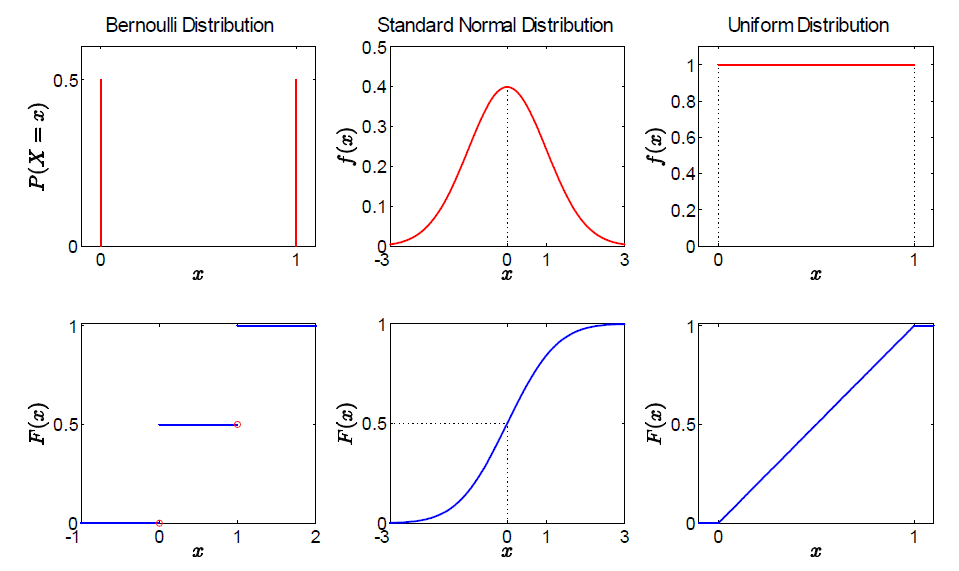
\includegraphics[width=0.9\textwidth]{figures/distributions}}\label{f1}
\end{figure}

\newpage

\subsection*{Discrete distributions}
\definitionbox{Bernoulli distribution}{
The $\textbf{Bernoulli distribution}$ for a single binomial outcome (trial) is
\begin{eqnarray*}
  Prob(x = 1) &=& p, \\
  Prob(x = 0) &=& 1-p,
\end{eqnarray*}
where $0 \leq p \leq 1$ is the probability of success.\\[-20pt]
\begin{itemize}
	\item  $E[x]=p$ and
	\item $V[x]=E[x^2]-E[x]^2=p-p^2=p(1-p)$.
\end{itemize}
 The distribution for $x$ successes in $n$ trials is the $\textbf{binomial distribution}$,\\[-5pt]
\begin{equation*}
    Prob(X = x) =\frac{n!}{(n-x)!x!}p^{x}(1-p)^{n-x}~~~x =0, 1,\ldots, n.
\end{equation*}
The mean and variance of $x$ are\\[-20pt]
\begin{itemize}
	\item  $E[x]=np$ and
	\item $V[x]=np(1 - p)$.
\end{itemize} }

Example of a binomial $[n=15,p=0.5]$ distribution:

\begin{figure}[H]
\begin{center}
%\scalebox{.36}
{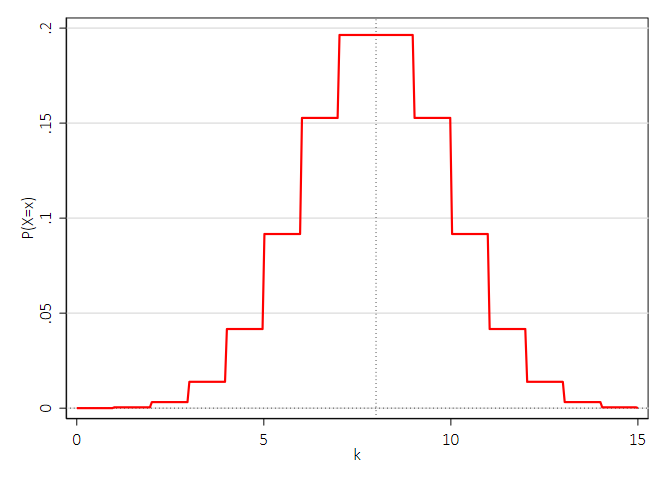
\includegraphics[width=0.45\textwidth]{figures/binomial_pdf}
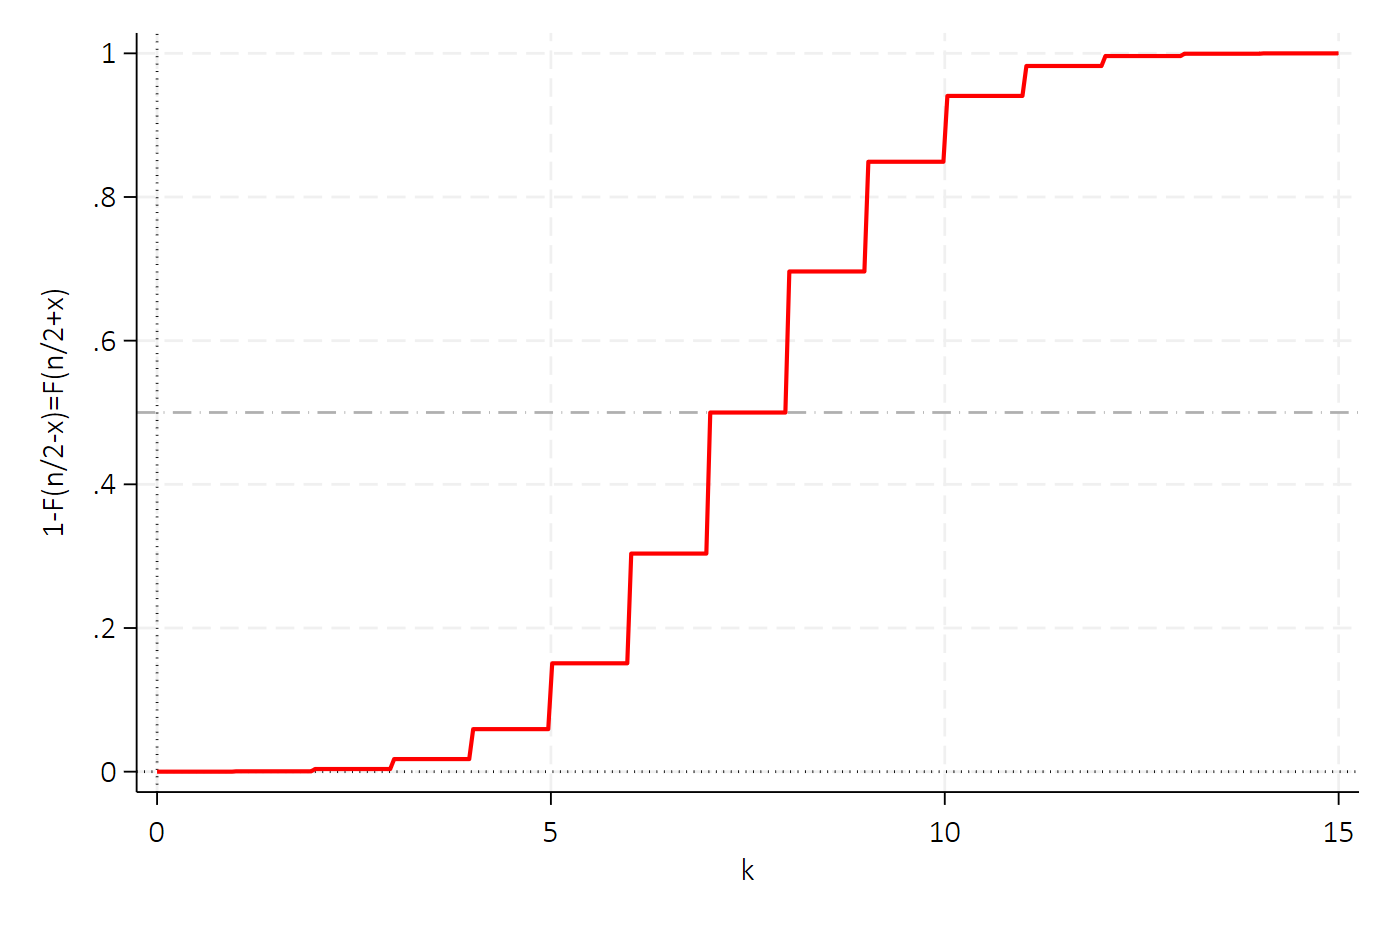
\includegraphics[width=0.45\textwidth]{figures/binomial_cdf}}\label{f2}
\end{center}
\end{figure}

\definitionbox{Poisson distribution}{

The limiting form of the binomial distribution, $n\rightarrow\infty$, is the $\textbf{Poisson distribution}$,
\begin{equation*}
    Prob(X = x) =\frac{e^{\lambda}\lambda^{x}}{x!}.
\end{equation*}
The mean and variance of $x$ are
\begin{itemize}
	\item  $E[x]=\lambda$ and
	\item $V[x]=\lambda$.
\end{itemize}}
\vspace{-10pt}
Example of a Poisson $[3]$ distribution:

\begin{figure}[H]
\begin{center}
%\scalebox{.36}
{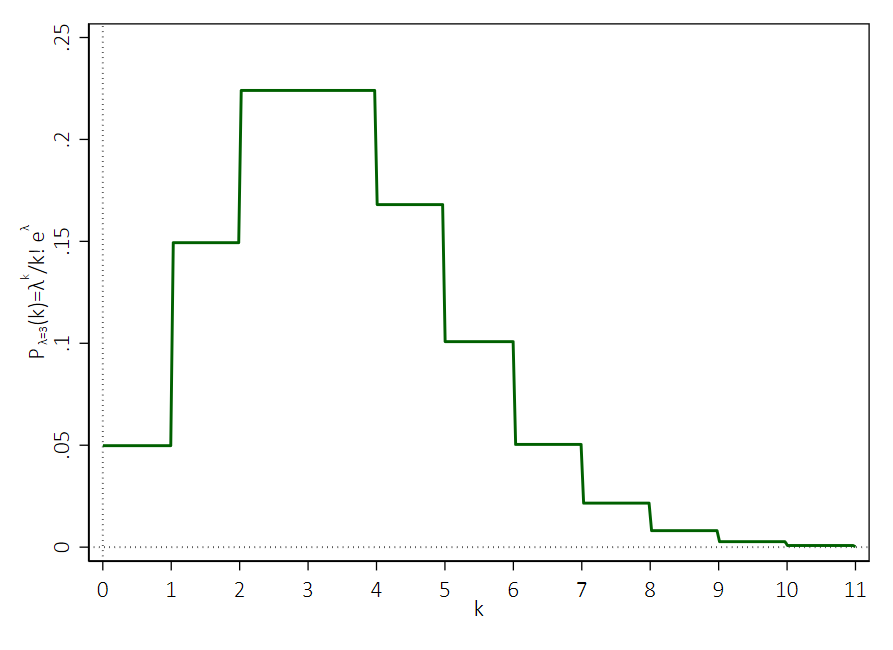
\includegraphics[width=0.9\textwidth]{figures/poisson_pdf}}\label{f4}
\end{center}
\end{figure}

\newpage

\subsection{Normal distribution}

\definitionbox{The normal distribution}{
Random variable $x \sim N[\mu, \sigma^{2}]$ is distributed according to the $\textbf{normal distribution}$ with mean $\mu$ and standard deviation $\sigma$ obtained as
\begin{equation*}
    f(x|\mu, \sigma)=\frac{1}{\sigma\sqrt{2\pi}}e^{-\frac{1}{2}(\frac{x-\mu}{\sigma})^2}.
\end{equation*}}

The density is denoted $\phi(x)$ and the cumulative distribution function is denoted $\Phi(x)$ for the standard normal. Example of a standard normal, ($x\sim N[0, 1]$), and a normal with mean $0.5$ and standard deviation $1.3$:

\begin{figure}[H]
\begin{center}
%\scalebox{.36}
{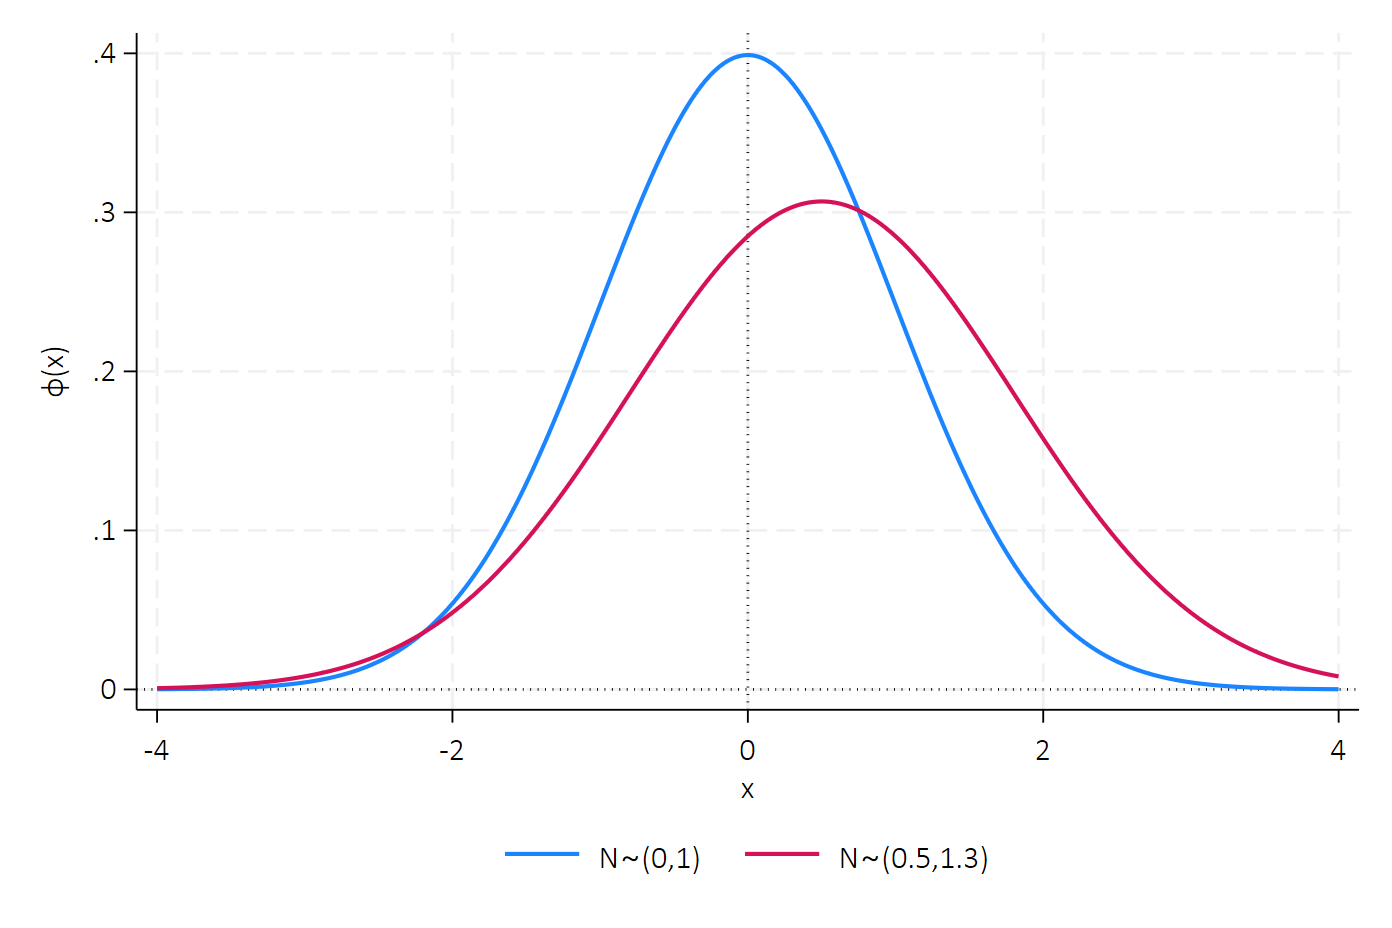
\includegraphics[width=0.9\textwidth]{figures/normals_pdf}}\label{f4}
\end{center}
\end{figure}



\subsection{Method of transformations}

\definitionbox{Transformation of random variables}{


Continuous variable $x$ may be transformed to a discrete variable $y$. Calculate the mean of variable $x$ in the respective interval:
\begin{eqnarray*}
  Prob(Y = \mu_{1}) &=& P(-\infty < X \leq a), \\
  Prob(Y = \mu_{2})  &=& P(a < X \leq b), \\
  Prob(Y = \mu_{3})  &=& P(b < X \leq \infty).\\
\end{eqnarray*}}


\definitionbox{Method of transformations}{
\renewcommand{\baselinestretch}{1.}

If $x$ is a continuous random variable with pdf $f_{x}(x)$ and if $y = g(x)$ is a continuous monotonic function of $x$, then the density of $y$ is obtained by
\begin{equation*}
    Prob(y \leq b) =\int_{-\infty}^{b}f_{x}(g^{-1}(y))|g^{-1\prime}(y)|dy.
\end{equation*}
With $f_{y}(y)=f_{x}(g^{-1}(y))|g^{-1\prime}](y)|dy$, this equation can be written as
$$Prob(y \leq b) =\int_{-\infty}^{b}f_{y}(y)dy.$$}

\examplebox{Example}{
If $x \sim N[\mu, \sigma^{2}],$ then the distribution of $y=g(x)=\frac{x-\mu}{\sigma}$ is found as follows:
$$g^{-1}(y)= x=\sigma y+\mu$$
$$g^{-1\prime}(y)= \frac{dx}{dy}=\sigma$$
Therefore with $f_x(x)=\frac{1}{\sigma\sqrt{2\pi}}e^{-\frac{1}{2}[(g^{-1}(y)-\mu)^2/\sigma^{2}]}|g^{-1\prime}(y)|$
\begin{equation*}
    f_{y}(y)=\frac{1}{\sqrt{2\pi}\sigma}e^{-[(\sigma y+\mu)-\mu]^{2}/2\sigma^{2}}|\sigma|=\frac{1}{\sqrt{2\pi}}e^{-y^{2}/2}.
\end{equation*}
}



\subsubsection*{Properties of the normal distribution}


\begin{itemize}
	\item Preservation under linear transformation:\\
 If $x \sim N[\mu, \sigma^{2}],$ then $(a + bx) \sim N[a + b\mu, b^{2}\sigma^{2}].$
\item Convenient transformation $a = -\mu/\sigma$ and $b = 1/\sigma$:\\
 The resulting variable $z=\frac{(x - \mu)}{\sigma}$ has the standard normal distribution with density $$\phi(z)=\frac{1}{\sqrt{2\pi}}e^{-\frac{z^{2}}{2}}.$$
\item If $x \sim N[\mu,\sigma^{2}]$, then $f(x)=\frac{1}{\sigma}\phi[\frac{x-\mu}{\sigma}]$
\item $Prob(a \leq x \leq b) = Prob\left(\frac{a-\mu}{\sigma}\leq\frac{x-\mu}{\sigma}\leq\frac{b-\mu}{\sigma}\right)$
\item $\phi(-z) = 1 - \phi(z)$ and $\Phi(-x)=1-\Phi(x)$ because of symmetry
\end{itemize}




If $z \sim N[0, 1]$, then $z^{2} \sim \chi^2[1]$ with pdf $\frac{1}{\sqrt{2\pi y}}e^{-y/2}$.\\

\examplebox{Example}{\renewcommand{\baselinestretch}{0.9}

$$f_x(x)=\frac{1}{\sqrt{2\pi}}e^{-\frac{x^2}{2}}$$
$$y=g(x)=x^2$$
$$g^{-1}(y)= x=\pm \sqrt{y} \text{ there are two solutions to } g_1,g_2.$$
$$g^{-1\prime}(y)= \frac{dx}{dy}=\pm 1/2y^{-1/2}$$
$$f_{y}(y)=f_x(g_1^{-1}(y))|g_1^{-1\prime}(y)|+f_x(g_2^{-1}(y))|g_2^{-1\prime}(y)|$$
$$f_{y}(y)=f_x(\sqrt{y})|1/2y^{-1/2}|+f_x(-\sqrt{y})|-1/2y^{-1/2}|$$
$$f_{y}(y)=\frac{1}{2\sqrt{2\pi y}}e^{-\frac{y}{2}}+\frac{1}{2\sqrt{2\pi y}}e^{-\frac{y}{2}}=\frac{1}{\sqrt{2\pi y}}e^{-\frac{y}{2}}$$
}


\begin{table}[h!]
%\vspace{-2mm}\centering
{
%\begin{tabular}{l*{5}{D{.}{.}{-1}}}

\begin{tabular}{@{\extracolsep{4pt}}l*{4}{l}}
\toprule
 & Normal \\
\midrule
Parameters &$\mu\in\mathbb{R}$ , $\sigma\in\mathbb{R}_{>0}$      \\
Support    & $x\in\mathbb{R}$                                          \\
PDF        & $\phi\left(\frac{x-\mu}{\sigma}\right)=\frac{1}{\sigma\sqrt{2\pi}} e^{-\frac{1}{2}\left(\frac{x - \mu}{\sigma}\right)^2}$ \\
CDF        & $\Phi\left(\frac{x-\mu}{\sigma}\right) = \frac{1}{2}\left[1 + \operatorname{erf}\left( \frac{x-\mu}{\sigma\sqrt{2}}\right)\right] $   \\
Mean       & $\mu$    \\
Median     & $\mu$  \\
Mode       & $\mu$      \\
Variance   & $\sigma^2$   \\
Skewness   &  $0$ \\
Ex. Kurtosis   &  $0$     \\
MGF        &  $\exp(\mu t + \sigma^2t^2/2)$  \\
\bottomrule
\end{tabular}

\begin{itemize}

\item PDF denotes probability density function, CDF cumulative distribution function, MGF moment-generating function.
\item $\mu$ mean (location), $\sigma, s$ (scale).
%\item $B(z_1,z_2)$ is beta function $\int_0^1 t^{z_1-1}(1-t)^{z_2-1}\,dt$ for complex number inputs $z_1, z_2$ with $\Re(z_1),\Re(z_2) > 0$.
\item Excess Kurtosis is defined as Kurtosis minus 3.
\item The Gauss error function is $\operatorname{erf} z = \frac{2}{\sqrt\pi}\int_0^z e^{-t^2}\,\mathrm dt.$
%\item $k, n_1, n_2$ known as ``degrees of freedom''.
%\item regularized incomplete beta function $I_x(a,b) = \frac{B(x;\,a,b)}{B(a,b)}.$

\end{itemize}
}

\end{table}





\subsubsection*{Distributions derived from the normal}

\begin{itemize}
  \item If $z \sim N[0, 1]$, then $z^{2} \sim \chi^2[1]$ with $E[z^2]=1$ and $V[z^2]=2$.
  \item If $x_{1},..., x_{n}$ are $n$ independent $\chi^2[1]$ variables, then $$\sum_{i=1}^{n}x_{i}\sim \chi^2[n].$$
  \item If $z_{i},i = 1,..., n,$ are independent $N[0, 1]$ variables, then $$\sum_{i=1}^{n}z_{i}^{2}\sim \chi^{2}[n].$$
  \item If $z_{i},i = 1,..., n$, are independent $N[0, \sigma^2]$ variables, then $$\sum_{i=1}^{n}\bigg(\frac{z_{i}}{\sigma}\bigg)^{2}\sim \chi^{2}[n].$$
  \item If $x_{1}$ and $x_{2}$ are independent $\chi^2$ variables with $n_{1}$ and $n_{2}$ degrees of freedom, then $$x_{1} + x_{2} \sim \chi^{2}[n_{1} + n_{2}].$$
\end{itemize}

\newpage

\subsection{The $\chi^2$ distribution}
\definitionbox{The $\chi^2$ distribution}{
Random variable $x \sim \chi^2[n]$ is distributed according to the $\textbf{ chi-squared distribution}$ with $n$ degrees of freedom
\begin{equation*}
    f(x|n)=\dfrac{x^{n/2 -1} e^{-x/2}}{2^{n/2} \Gamma\left(\frac n 2 \right)},
\end{equation*}

where $\Gamma$ is the Gamma-distribution (more below).
\begin{itemize}
	\item $E[x]=n$
  \item $V[x]=2n$
\end{itemize}}

Example of a $\chi^2[3]$ distribution:

\begin{figure}[H]
\begin{center}
%\scalebox{.36}
{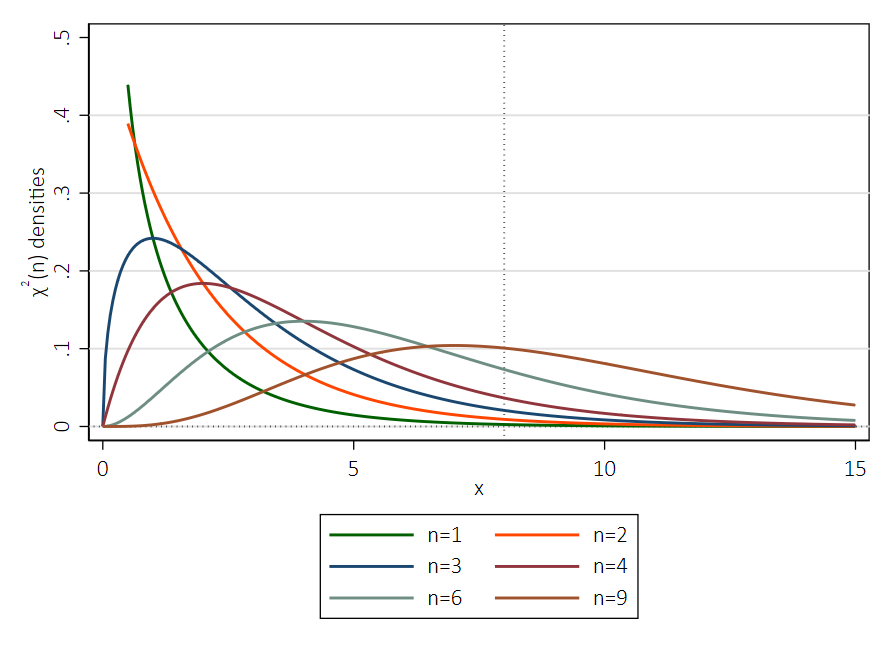
\includegraphics[width=0.49\textwidth]{figures/chi2_pdf}}
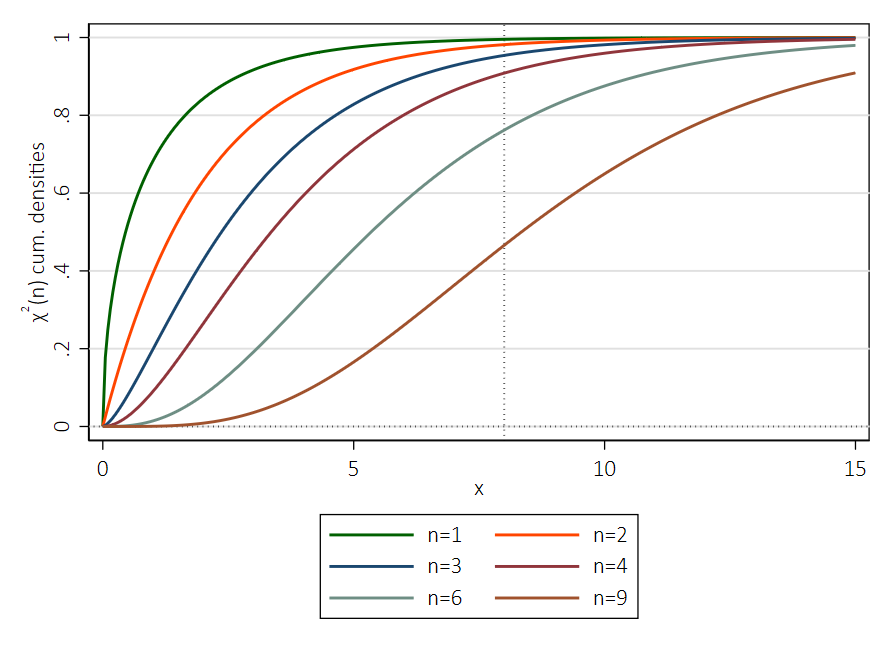
\includegraphics[width=0.49\textwidth]{figures/chi2_cdf}\label{f2}\end{center}
\end{figure}


\definitionbox{Approximating a $\chi^2$}{
For degrees of freedom greater than $30$ the distribution of the chi-squared variable $x$ is approx.
\begin{equation*}\label{eq13}
    z = (2x)^{1/2} - (2n - 1)^{1/2},
\end{equation*}
which is approximately standard normally distributed. Thus,
\begin{equation*}
    Prob(\chi^{2}[n] \leq a) \approx \Phi[(2a)^{1/2} - (2n - 1)^{1/2}].
\end{equation*}}

\begin{figure}[H]
\begin{center}
%\scalebox{.36}
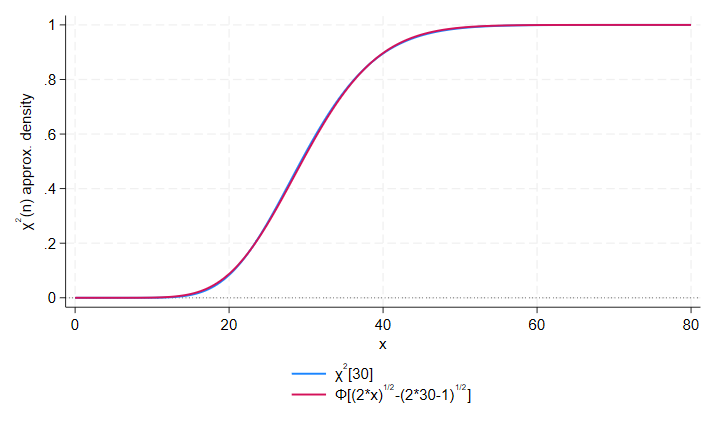
\includegraphics[width=0.9\textwidth]{figures/chi2_cdf_approx
}\label{ch1}
\end{center}
\end{figure}



\begin{table}[H]
%\vspace{-5mm}
\centering
{
%\begin{tabular}{l*{5}{D{.}{.}{-1}}}

\begin{tabular}{@{\extracolsep{4pt}}l*{4}{l}}
\toprule
 & $\chi^2$ \\
\midrule
Parameters & $n\in\mathbb{N}_{>0}$     \\
Support    & $x\in\mathbb{R}_{>0}\;$ if $n = 1,$       \\
           &  else $x \in\mathbb{R}_{\geq0}$      \\
PDF        & $\frac{1}{2^{n/2}\Gamma(n/2)}\; x^{n/2-1} e^{-x/2}\; $     \\
CDF        &  $\frac{1}{\Gamma(n/2 )} \; \gamma\left(\frac{n}{2},\,\frac{x}{2}\right)\;$  \\
Mean       & $n$      \\
Median     &   No simple closed form      \\
Mode       &   $\max(n-2,0)\;$     \\
Variance   &   $2n\;$    \\
Skewness   &  $\sqrt{8/n}\,$     \\
Ex. Kurtosis   &  $\frac{12}{n}$ \\
MGF        &    $(1-2t)^{-n/2} \text{ for } t < \frac{1}{2}\;$     \\
\bottomrule
\end{tabular}

\begin{itemize}

\item $n, n_1, n_2$ known as degrees of freedom.
\item Regularized incomplete beta function $I(x,a,b) = \frac{B(x,\,a,b)}{B(a,b)}$ with $B(x,\,a,b) = \int_0^x t^{a-1}\,(1-t)^{b-1}\,dt.$

\end{itemize}
}

\end{table}


\newpage


\subsection{The F-distribution}
\definitionbox{The F-distribution}{
If $x_{1}$ and $x_{2}$ are two independent chi-squared variables with degrees of freedom parameters
   $n_{1}$ and $n_{2}$, respectively, then the ratio
   \begin{equation*}\label{eq11}
    F [n_{1}, n_{2}] = \frac{x_{1}/n_{1}}{x_{2}/n_{2}}
   \end{equation*}
   has the $\textbf{F distribution}$ with $n_{1}$ and $n_{2}$ degrees of freedom.}

\begin{figure}[H]
\begin{center}
%\scalebox{.36}
{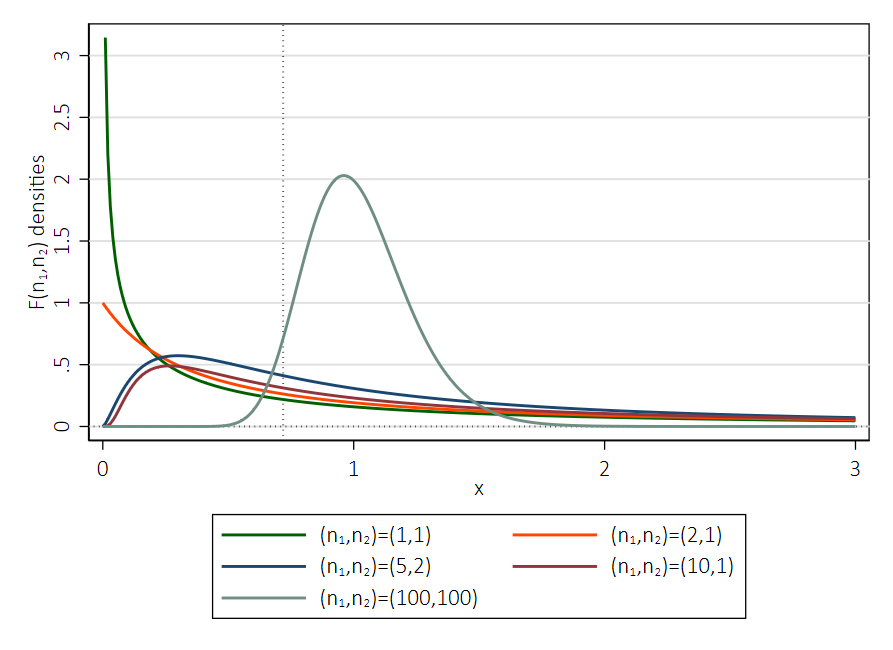
\includegraphics[width=0.49\textwidth]{figures/F_pdf}
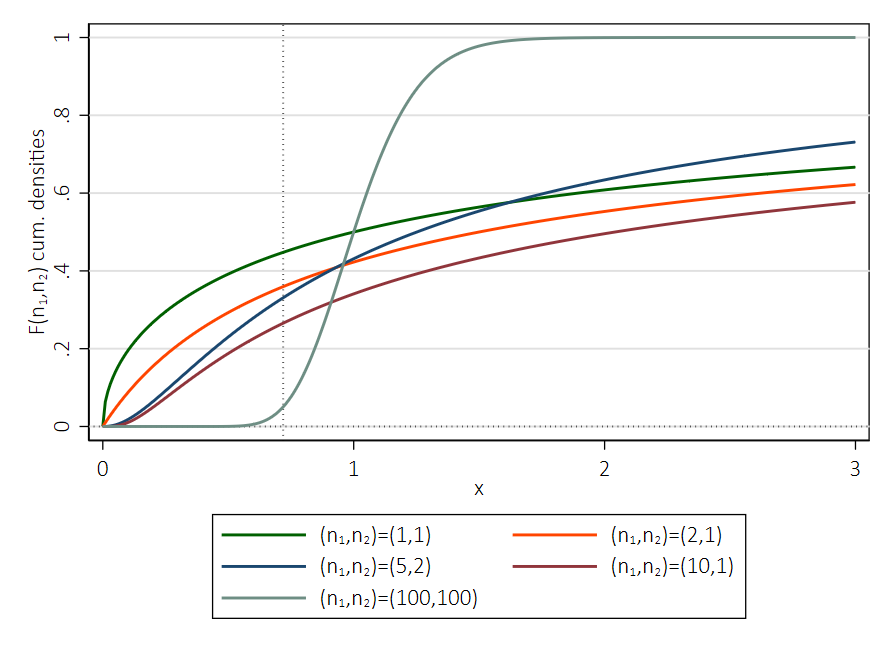
\includegraphics[width=0.49\textwidth]{figures/F_cdf}}\label{f3}
\end{center}
\end{figure}


\begin{table}[H]
%\vspace{-5mm}
\centering
{
%\begin{tabular}{l*{5}{D{.}{.}{-1}}}

\begin{tabular}{@{\extracolsep{4pt}}l*{4}{l}}
\toprule
 & $F$ \\
\midrule
Parameters & $n_1$, $n_2\in\mathbb{N}_{>0}$    \\
Support    & $x\in\mathbb{R}_{>0}\;$ if $n_1 = 1$,    \\
           & else $x \in\mathbb{R}_{\geq0}$   \\
PDF        & $n_1^{\frac{n_1}{2}} n_2^{\frac{n_2}{2}}  \frac{\Gamma (\frac{n_1+n_2}{2})}{\Gamma (\frac{n_1}{2}) \Gamma (\frac{n_2}{2})}  \frac{x^{\frac{n_1}{2}-1}}{(n_1x+n_2)^\frac{n_1+n_2}{2}}$    \\
CDF        &    $I\left(\frac{n_1 x}{n_1 x + n_2},\,\tfrac{n_1}{2}, \tfrac{n_2}{2} \right)$   \\
Mean       & $\frac{n_2}{n_2-2}\!$ for $n_2 > 2$    \\
Median     &    No simple closed form     \\
Mode       &  $\frac{n_1-2}{n_1}\;\frac{n_2}{n_2+2}$ for $n_1 > 2$    \\
Variance   &    $\frac{2\,n_2^2\,(n_1+n_2-2)}{n_1 (n_2-2)^2 (n_2-4)}\!$ for $n_2 > 4$     \\
Skewness   &  $\frac{(2 n_1 + n_2 - 2) \sqrt{8 (n_2-4)}}{(n_2-6) \sqrt{n_1 (n_1 + n_2 -2)}}\!$for $n_2 > 6$    \\
Ex. Kurtosis   &  $12\frac{n_1(5n_2-22)(n_1+n_2-2)+(n_2-4)(n_2-2)^2}{n_1(n_2-6)(n_2-8)(n_1+n_2-2)}$ for $n_2>8$ \\
MGF        &    does not exist    \\
\bottomrule
\end{tabular}

\begin{itemize}

\item $n, n_1, n_2$ known as degrees of freedom.
\item Regularized incomplete beta function $I(x,a,b) = \frac{B(x,\,a,b)}{B(a,b)}$ with $B(x,\,a,b) = \int_0^x t^{a-1}\,(1-t)^{b-1}\,dt.$

\end{itemize}
}

\end{table}


\newpage

\subsection{The student t-distribution}
\definitionbox{The student t-distribution}{
If $x_1$ is an $N[0, 1]$ variable, often denoted by $z$, and $x_2$ is $\chi^{2}[n_2]$ and is independent of $x_1$, then the ratio
  \begin{equation*}\label{eq12}
    t[n_2] = \frac{x_1}{\sqrt{x_2/n_2}}.
  \end{equation*}
  has the $\textbf{t distribution}$ with $n_2$ degrees of freedom.}

Example for the $t$ distributions with $3$ and $10$ degrees of freedom with the standard normal distribution.
\begin{figure}[H]
\begin{center}
%\scalebox{.36}
{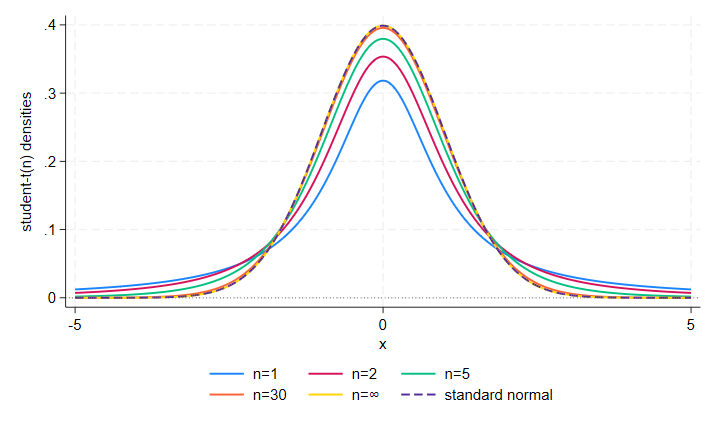
\includegraphics[width=0.49\textwidth]{figures/t_pdf}
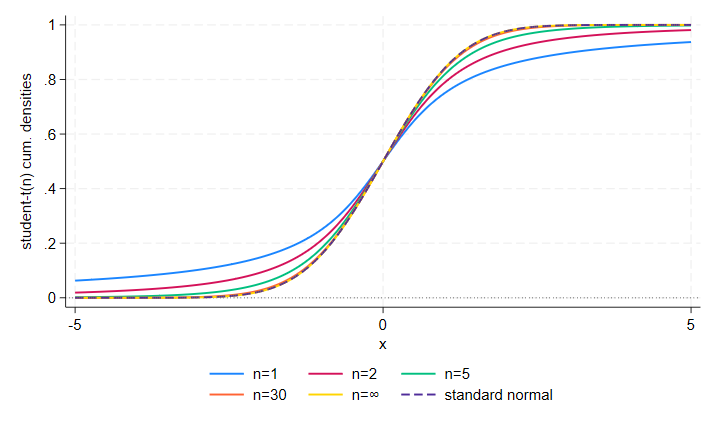
\includegraphics[width=0.49\textwidth]{figures/t_cdf}}\label{f3}
\end{center}
\end{figure}

Comparing (\ref{eq11}) with $n_{1} = 1$ and (\ref{eq12}), if $t \sim t[n]$, then $t^{2} \sim F[1, n]$.




The $t[30]$ approx. the standard normal

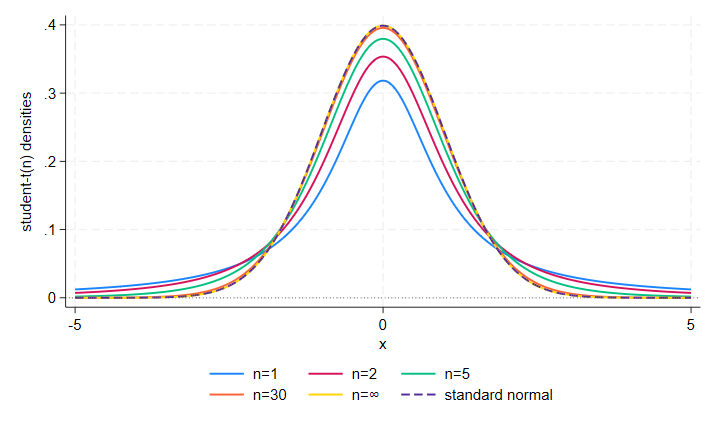
\includegraphics[width=0.9\textwidth]{figures/t_pdf}


\begin{table}[H]
%\vspace{-5mm}\centering
{
%\begin{tabular}{l*{5}{D{.}{.}{-1}}}

\begin{tabular}{@{\extracolsep{0pt}}l*{3}{l}}
\toprule
 & $t$    \\
\midrule
Parameters & $n\in\mathbb{R}_{>0} $      \\
Support    & $x \in\mathbb{R}$   \\
PDF        & $\frac{\Gamma \left(\frac{\ n+1\ }{ 2 } \right)} {\sqrt{\pi n\ }\ \Gamma \left(\frac{ n }{\ 2\ } \right)} \left(1 + \frac{x^2}{ n } \right)^{-\frac{\ n+1\ }{ 2 }}$   \\
CDF        & $\frac{\ 1\ }{ 2 } + x\ \Gamma \left( \frac{\ n+1\ }{ 2 } \right) \times $
      \\
           & $ \frac{{ {}_{2}F_1 }\!\left(\frac{\ 1\ }{ 2 },\ \frac{\ n+1\ }{ 2 };\ \frac{ 3 }{\ 2\ };\
           -\frac{~ x^2\ }{ n }\right)}  {\sqrt{\pi n}\ \Gamma \left(\frac{n}{ 2 }\right)}$
    \\
Mean       & $\ 0\ $ for $\ n > 1\ $  \\
Median     & $\ 0\ $   \\
Mode       & $\ 0\ $   \\
Variance   & $\frac{ n }{\ n-2\ }\ $ for $\ n > 2,$  \\
   & $\infty$ for $1 < n \le 2$    \\
Skewness   & $0$ for $n > 3$    \\
Ex. Kurtosis   & $\frac{ 6 }{n-4}$ for $n > 4, \infty$ for $2 < n \le 4$   \\
MGF        & does not exist  \\
\bottomrule
\end{tabular}

\begin{itemize}

\item $n$ denote degrees of freedom.
\item $\ {}_{2}F_1\!(\cdot,\cdot;\cdot;\cdot)\ $ is a particular instance of the hypergeometric function.

\end{itemize}
}

\end{table}



\newpage

\subsection{The lognormal distribution}

\definitionbox{The lognormal distribution}{
The $\textbf{lognormal distribution}$, denoted $LN[\mu,\sigma^{2}]$, has been particularly
useful in modeling the size distributions.
\begin{equation*}
    f(x) = \frac{1}{\sqrt{2\pi}\sigma x}e^{-\frac{1}{2}[(\ln x-\mu)/\sigma]^{2}},~~~~~~~x>0
\end{equation*}
A lognormal variable $x$ has
\begin{itemize}
	\item  $E[x]= e^{\mu+\sigma^{2}/2},$ and
	\item $Var[x]= e^{2\mu+\sigma^{2}}(e^{\sigma^{2}}-1).$
\end{itemize}}

If $y \sim LN[\mu,\sigma^{2}],$ then $\ln y \sim N[\mu,\sigma^{2}].$
\begin{figure}[H]
\begin{center}
%\scalebox{.36}
{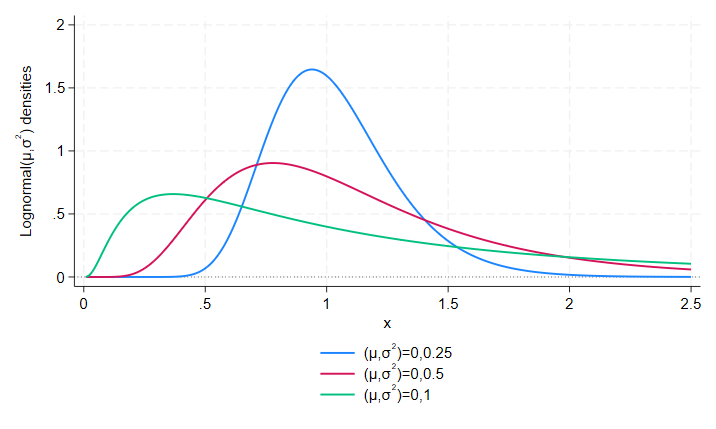
\includegraphics[width=0.49\textwidth]{figures/lnnormal_pdf}
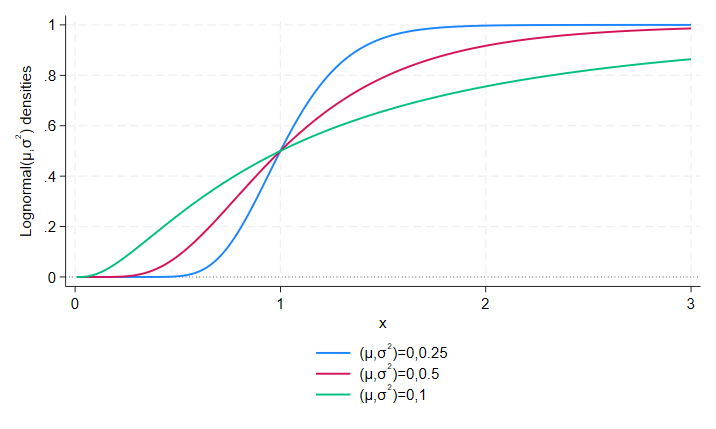
\includegraphics[width=0.49\textwidth]{figures/lnnormal_cdf}}\label{f2}
\end{center}
\end{figure}


\begin{table}[H]
%\vspace{-5mm}\centering
{
%\begin{tabular}{l*{5}{D{.}{.}{-1}}}

\begin{tabular}{@{\extracolsep{0pt}}l*{3}{l}}
\toprule
 & Log-normal   \\
\midrule
Parameters &  $\mu \in\mathbb{R}$ , $\sigma\in\mathbb{R}_{>0}$    \\
Support    &  $x \in\mathbb{R}_{>0}$   \\
PDF        &  $\frac{ 1 }{\ x\sigma\sqrt{2\pi\ }\ }\ \exp\left( - \frac{ \left( \ln x  - \mu\ \right)^2}{ 2 \sigma^2 } \right)$   \\
CDF        &  $\ \frac{\ 1\ }{2}\left[1 + \operatorname{erf}\left( \frac{\ \ln x - \mu\ }{\sigma\sqrt{2\ }} \right)\right] $   \\
           & $= \Phi\left(\frac{\ln(x) -\mu}{\sigma} \right)$\\
Mean       &  $\ \exp\left(\mu + \frac{\sigma^2}{2}\right)\ $ \\
Median     &  $\ \exp(\mu)\ $  \\
Mode       &  $\ \exp\left(\mu - \sigma^2\right)\ $   \\
Variance   & $\left[\exp(\sigma^2) - 1\right]\exp\left( 2\mu + \sigma^2\right )$   \\
Skewness   & $\left[\exp\left( \sigma^2 \right) + 2\right] \sqrt{\exp(\sigma^2) - 1}$   \\
Ex. Kurtosis   & $1\exp\left(4\sigma^2 \right) + 2\exp\left(3\sigma^2 \right) + 3\exp\left(2\sigma^2 \right) - 6$   \\
MGF        & not determined by its moments  \\
\bottomrule
\end{tabular}


}

\end{table}


\newpage

\subsection{The gamma distribution}
\definitionbox{The gamma distribution}{
The general form of the $\textbf{gamma distribution}$ is
\begin{equation*}
    f(x) = \frac{\beta^{\alpha}}{\Gamma (\alpha)}e^{-\beta x}x^{\alpha-1},~~~~~~~x\geq0, \beta=1/\theta>0, \alpha=k>0.
\end{equation*}}

Many familiar distributions are special cases, including the $\textbf{exponential distribution} (\alpha = 1)$ and
$\textbf{chi-squared} (\beta = 1/2 , \alpha = n/2 )$. The $\textbf{Erlang distribution}$ results if $\alpha$ is a positive integer. The mean is
$\alpha/\beta$, and the variance is $\alpha/\beta^{2}$. The $\textbf{inverse gamma distribution}$ is the distribution of $1/x$, where $x$ has the gamma distribution.
\begin{figure}[H]
\begin{center}
%\scalebox{.36}
{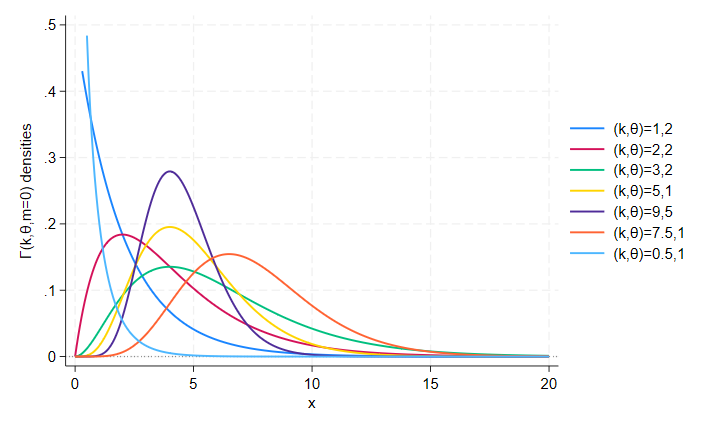
\includegraphics[width=0.49\textwidth]{figures/gamma_pdf}
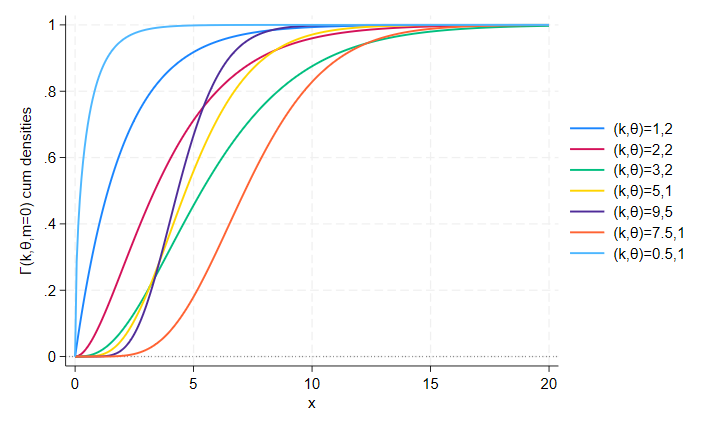
\includegraphics[width=0.49\textwidth]{figures/gamma_cdf}}\label{f2}
\end{center}
\end{figure}


\begin{table}[H]
%\vspace{-5mm}\centering
{
%\begin{tabular}{l*{5}{D{.}{.}{-1}}}

\begin{tabular}{@{\extracolsep{4pt}}l*{4}{l}}
\toprule
 & $\Gamma$ & $\Gamma$  \\
\midrule
Parameters & $k > 0\in\mathbb{R}$ (shape), & $\alpha > 0\in\mathbb{R}$ (shape), &  \\
           & $\theta > 0\in\mathbb{R}$ scale & $\beta > 0\in\mathbb{R}$ (rate) &  \\
Support    & $x \in\mathbb{R}(0, \infty)$ & $x \in\mathbb{R}(0, \infty)$ &  \\
           &  &  &  \\
PDF        & $f(x)=\frac{1}{\Gamma(k) \theta^k} x^{k - 1} e^{-x/\theta}$ & $f(x)=\frac{\beta^\alpha}{\Gamma(\alpha)} x^{\alpha - 1} e^{-\beta x }$ &  \\
CDF        & $F(x)=\frac{1}{\Gamma(k)} \gamma\left(k, \frac{x}{\theta}\right)$ & $F(x)=\frac{1}{\Gamma(\alpha)} \gamma(\alpha, \beta x)$ &  \\
Mean       & $k \theta $ & $\frac{\alpha}{\beta}$ &  \\
Median     & No simple closed form &  No simple closed form &  \\
Mode       & $(k - 1)\theta \text{ for } k \geq 1$, $0 \text{ for } k < 1$ & $\frac{\alpha - 1}{\beta} \text{ for } \alpha \geq 1\text{, }0 \text{ for } \alpha < 1$ &  \\
Variance   & $k \theta^2$ & $\frac{\alpha}{\beta^2}$ &  \\
Skewness   & $\frac{2}{\sqrt{k}}$ & $\frac{2}{\sqrt{\alpha}}$ &  \\
Ex. Kurtosis   & $\frac{6}{k}$ & $\frac{6}{\alpha}$ &  \\
MGF        & $(1 - \theta t)^{-k} \text{ for } t < \frac{1}{\theta}$ & $\left(1 - \frac{t}{\beta}\right)^{-\alpha} \text{ for } t < \beta$ &  \\
\bottomrule
\end{tabular}

\begin{itemize}

\item $\Gamma(z) = \int_0^\infty t^{z-1} e^{-t}\text{ d}t, \qquad \Re(z) > 0$, for complex numbers with a positive real part.
\item lower incomplete gamma function is $\gamma(s,x) = \int_0^x t^{s-1}\,e^{-t}\, dt$, for complex numbers with a positive real part.

\end{itemize}
}

\end{table}

\newpage

\subsection{The beta distribution}
\definitionbox{The beta distribution}{
For a variable constrained between $0$ and $c > 0$, the $\textbf{beta distribution}$ has proved useful. Its density is
\begin{equation*}
    f(x) = \frac{\Gamma(\alpha+\beta)}{\Gamma (\alpha)\Gamma(\beta)}\left(\frac{x}{c}\right)^{\alpha-1}\left(1-\frac{x}{c}\right)^{\beta-1}\frac{1}{c},~~~~~~~0\leq x\leq1.
\end{equation*}
It is symmetric if $\alpha = \beta$, asymmetric otherwise.  The mean is $ca/(\alpha + \beta)$,
and the variance is $c^{2}\alpha\beta/[(\alpha +\beta +1)(\alpha +\beta)^{2}]$.}
\begin{figure}[H]
\begin{center}
{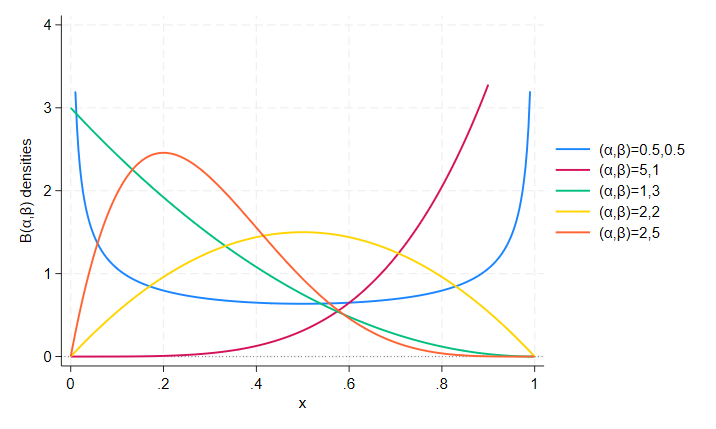
\includegraphics[width=0.49\textwidth]{figures/beta_pdf}
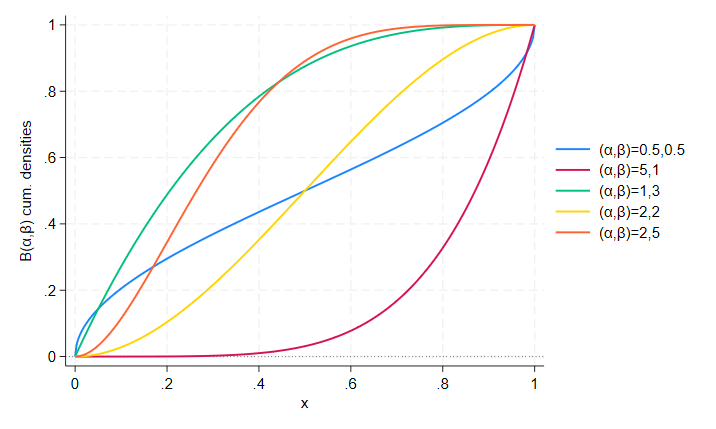
\includegraphics[width=0.49\textwidth]{figures/beta_cdf}}\label{f2}
\end{center}
\end{figure}

\begin{table}[H]
%\vspace{-5mm}\centering
{
%\begin{tabular}{l*{5}{D{.}{.}{-1}}}

\begin{tabular}{@{\extracolsep{4pt}}l*{4}{l}}
\toprule
 & $B$ &   \\
\midrule
Parameters & $\alpha, \beta\in\mathbb{R}_{>0}$  & \\
Support    & $x\in[0, 1]\!$ or $x \in (0, 1)\!$ &  \\
PDF        & $\frac{x^{\alpha-1}(1-x)^{\beta-1}} {B(\alpha,\beta)}\!$ &    \\
CDF        & $I(x,\,\alpha,\beta)\!$ &  &  \\
Mean       & $\frac{\alpha}{\alpha+\beta}\!$ &  \\
Median     & $\begin{matrix}I_{\frac{1}{2}}^{[-1]}(\alpha,\beta)\approx \frac{ \alpha - \tfrac{1}{3} }{ \alpha + \beta - \tfrac{2}{3} }\text{ for }\alpha, \beta >1\end{matrix}$  &  \\
Mode       & $^*$ & \\
Variance   & $\frac{\alpha\beta}{(\alpha+\beta)^2(\alpha+\beta+1)}\!$ &    \\
Skewness   & $\frac{2\,(\beta-\alpha)\sqrt{\alpha+\beta+1}}{(\alpha+\beta+2)\sqrt{\alpha\beta}}$ &    \\
Ex. Kurtosis   & $\frac{6[(\alpha - \beta)^2 (\alpha +\beta + 1) - \alpha \beta (\alpha + \beta + 2)]}{\alpha \beta (\alpha + \beta + 2) (\alpha + \beta + 3)}$  &  \\
MGF        & $1  +\sum_{k=1}^\infty \left( \prod_{r=0}^{k-1} \frac{\alpha+r}{\alpha+\beta+r} \right) \frac{t^k}{k!}$ & &  \\
\bottomrule
\end{tabular}

\begin{itemize}

\item $B(\alpha,\beta) = \frac{\Gamma(\alpha)\Gamma(\beta)}{\Gamma(\alpha + \beta)}$ and $\Gamma$ is the Gamma function.
\item $\Gamma(z) = \int_0^\infty t^{z-1} e^{-t}\text{ d}t, \qquad \Re(z) > 0$, for complex numbers with a positive real part.
\item Regularized incomplete beta function $I(x,\,a,b) = \frac{B(x,\,a,b)}{B(a,b)}$ with $B(x,\,a,b) = \int_0^x t^{a-1}\,(1-t)^{b-1}\,dt.$
\item  $^*\frac{\alpha-1}{\alpha+\beta-2}\, \text{for}\,\alpha, \beta > 1; \text{any value in} (0,1)\, \text{for }\,\alpha, \beta = 1; \{0, 1\}\, \text{(bimodal)}\, \text{for }\,\alpha, \beta < 1; 0\, \text{for }\,\alpha \leq 1, \beta > 1; 1\, \text{for }\,\alpha > 1, \beta \leq 1.$

\end{itemize}
}

\end{table}

\newpage

\subsection{The logistic distribution}
\definitionbox{The logistic distribution}{
The $\textbf{logistic distribution}$ is an alternative if the normal cannot model the mass in the tails; the cdf for a logistic random variable with $\mu=0, s=1$ is
\begin{equation*}
    F(x) =\Lambda(x)= \frac{1}{1+e^{-x}}.
\end{equation*}
The density is $f(x) = \Lambda(x)[1 - \Lambda(x)]$. The mean and variance of this random variable are zero
and $\sigma^2=\pi^{2}/3$.}
\begin{figure}[H]
\begin{center}
{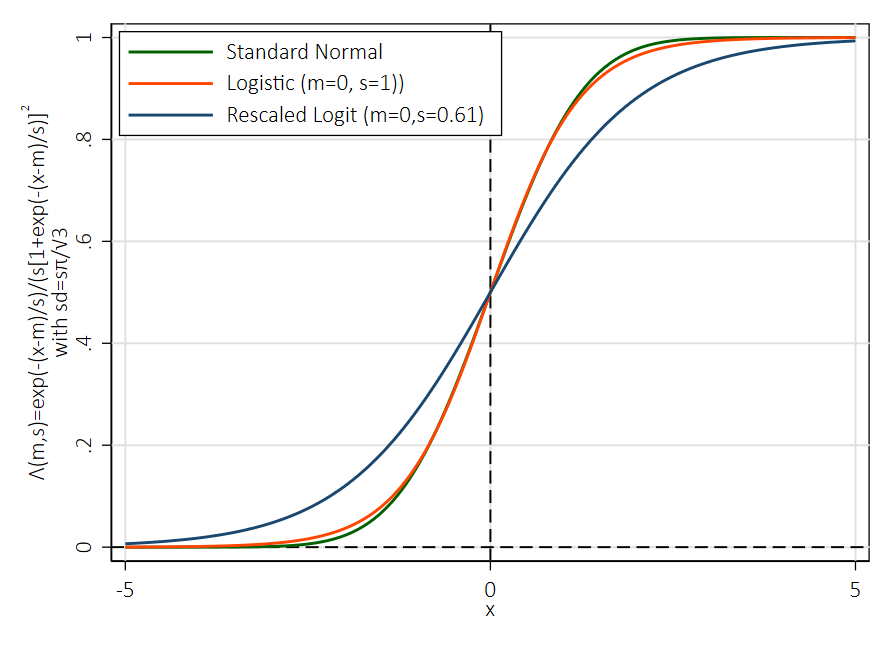
\includegraphics[width=0.9\textwidth]{figures/normal_logistic_cdf}}\label{f2}
\end{center}
\end{figure}



\begin{table}[h!]
%\vspace{-2mm}\centering
{
%\begin{tabular}{l*{5}{D{.}{.}{-1}}}

\begin{tabular}{@{\extracolsep{4pt}}l*{4}{l}}
\toprule
 & Logistic \\
\midrule
Parameters &$\mu\in\mathbb{R}$ , $s\in\mathbb{R}_{>0}$   \\
Support    &  $x \in \mathbb{R}$    \\
PDF        &  $\lambda\left(\frac{x-\mu}{s}\right)=\frac{e^{-(x-\mu)/s}} {s\left(1+e^{-(x-\mu)/s}\right)^2}$ \\
CDF        & $\Lambda\left(\frac{x-\mu}{s}\right)=\frac{1}{1+e^{-(x-\mu)/s}}$ \\
Mean       & $\mu$   \\
Median     &  $\mu$     \\
Mode       &   $\mu$    \\
Variance   &  $\frac{s^2 \pi^2}{3}$      \\
Skewness   &  $0$ \\
Ex. Kurtosis   &   $6/5$    \\
MGF        &    $e^{\mu t}B(1-st, 1+st)$    \\
           &  for $t \in (-1/s,1/s)$   \\
\bottomrule
\end{tabular}

%\begin{itemize}

%\item PDF denotes probability density function, CDF cumulative distribution function, MGF moment-generating function.
%\item $\mu$ mean (location), $\sigma, s$ (scale).
%\item $B(z_1,z_2)$ is beta function $\int_0^1 t^{z_1-1}(1-t)^{z_2-1}\,dt$ for complex number inputs $z_1, z_2$ with $\Re(z_1),\Re(z_2) > 0$.
%\item Excess Kurtosis is defined as Kurtosis minus 3.
%\item $k, n_1, n_2$ known as ``degrees of freedom''.
%\item regularized incomplete beta function $I_x(a,b) = \frac{B(x;\,a,b)}{B(a,b)}.$

%\end{itemize}
}

\end{table}


\newpage


\subsection{The Wishart distribution}
\definitionbox{The Wishart distribution}{ The $\textbf{Wishart distribution}$ describes the distribution of a random matrix obtained as
\begin{equation*}
    f(\bm{W}) =\sum_{i=1}^{n}(x_{i}-\mu)(x_{i}-\mu)^{\prime}.
\end{equation*}
where $x_{i}$ is the $i$th of $n K$ element random vectors from the multivariate normal distribution with
mean vector, $\mu$, and covariance matrix, $\Sigma$.  The density of the Wishart random matrix is
\begin{equation*}
    f(\bm{W}) =\frac{\exp\left[-\frac{1}{2}trace(\Sigma^{-1}\bm{W})\right]|\bm{W}|^{-\frac{1}{2}(n-K-1)}}{2^{nK/2}|\Sigma|^{K/2}\pi^{K(K-1)/4}\prod_{j=1}^{K}\Gamma\left(\frac{n+1-j}{2}\right)}.
\end{equation*}
The mean matrix is $n\Sigma$. For the individual pairs of elements in $\bm{W}$,
\begin{equation*}
    Cov[w_{ij}, w_{rs}] = n(\sigma_{ir}\sigma_{js} + \sigma_{is}\sigma_{jr}).
\end{equation*}
The Wishart distribution is a multivariate extension of $\chi^2$ distribution. If $\bm{W}\sim W(n,\sigma^2)$, then $\bm{W}/\sigma^2\sim\chi^2[n].$}







\clearpage
\section{Review of Distribution Theory}
\label{sec: Review of Distribution Theory}

\subsection{Joint and marginal bivariate distributions}



\subsubsection*{Bivariate distributions}
 For observations of two discrete variables $y\in\{1,2\}$ and $x\in\{1,2,3\}$, we can calculate
\begin{itemize}
	\item the frequencies $n_{x,y}$,
\end{itemize}
%\begin{example}
%-------------------------------------------
%\begin{landscape}

	
		\begin{table}[H]
        \centering
%\caption{Timeline of German Reforms}
\label{tab:timeline}

		\begin{tabular}{lrrr}
\cmidrule(r){1-4}
freq. $n_{x,y}$ &$y=1$ &$y=2$ &$f(x)=n_{x}/N$ \\
\cmidrule(r){1-4}
$x=1$ &1 &2 &3/10  \\
$x=2$ &1 &2 &3/10 \\
$x=3$ &0 &4 &4/10 \\
$f(y)=n_{y}/N$ &2/10 &8/10 &1 \\
\cmidrule(r){1-4}
\end{tabular}

	\end{table}


%\end{landscape}
%-------------------------------------------
%\end{example}




%
%
 %For observations of two discrete variables $y\in\{1,2\}$ and $x\in\{1,2,3\}$, we can calculate
%\begin{itemize}
	%\item the frequencies $n_{x,y}$,
	%\item conditional distributions $f(y|x)$ and $f(x|y)$,
%\end{itemize}
%%\begin{example}
%%-------------------------------------------
%%\begin{landscape}
%
	%\begin{center}
		%\begin{threeparttable}[htbp]
%%\caption{Timeline of German Reforms}
%\label{tab:timeline}
%
		%\resizebox{\textwidth}{!}{\begin{tabular}{l@{\extracolsep{-2mm}}rrrr@{\extracolsep{0pt}}l@{\extracolsep{-2mm}}rrr}
%\cmidrule(r){1-4}\cmidrule(r){6-9}
%freq. $n_{x,y}$ &$y=1$ &$y=2$ &$f(x)=n_{x}/N$ &	& cond. distr. $f(y|x)$ &$y=1$ &$y=2$ &$\sum_y $                              \\
%\cmidrule(r){1-4}\cmidrule(r){6-9}
%$x=1$ &1 &2 &3/10  & &	$f(y|x=1)$ &1/3 &2/3 &1                                                                                    \\
%$x=2$ &1 &2 &3/10  &	& $f(y|x=2)$ &1/3 &2/3 &1                                                                                   \\
%$x=3$ &0 &4 &4/10  &	& $f(y|x=3)$ &0   & 1  &1                                                                                   \\
%$f(y)=n_{y}/N$ &2/10 &8/10 &1 & &	$f(y|x=1,x=2,x=3) $ &1/5  &4/5 &1                                                                             \\
%\cmidrule(r){1-4}\cmidrule(r){6-9}
 %&	 &	 &	 &	 &	                                                                                                             \\
%\cmidrule(r){1-4}
%cond. distr.  &  & &  &	 &	\textcolor{white}{joint distr.}  &  &  &\textcolor{white}{marginal pr.}     \\
 %$f(x|y)$ &$f(x|y=1)$ &$f(x|y=2)$ &$f(x|y=1,y=2)$ & &	\textcolor{white}{$f(y,x)$} &\textcolor{white}{$f(y=1,x)$} &\textcolor{white}{$f(y=2,x)$}  &  \textcolor{white}{$f_x(x)$}    \\
%\cmidrule(r){1-4}
%$x=1$ &1/2  &1/4 &3/10 & &	\textcolor{white}{$f(y,x=1)$} &\textcolor{white}{1/10}  &\textcolor{white}{2/10} &\textcolor{white}{3/10}                                                                \\
%$x=2$ &1/2  &1/4 &3/10 & &	\textcolor{white}{$f(y,x=2)$} &\textcolor{white}{1/10}   &\textcolor{white}{2/10} &\textcolor{white}{3/10}                                                             \\
%$x=3$ &0  &1/2 &4/10 & &	\textcolor{white}{$f(y,x=3)$}   &\textcolor{white}{0}      &\textcolor{white}{4/10} &\textcolor{white}{4/10}                                                             \\
%$\sum_x $ &1 &1  &1 &	& \textcolor{white}{marginal pr. $f_y(y)$}    &\textcolor{white}{2/10}  &\textcolor{white}{8/10} &\textcolor{white}{1}                                            \\
%\cmidrule(r){1-4}
%\end{tabular}}
		%%\begin{tablenotes}
			%%\item \emph{Notes:}  the historical development of the regulatory measures. The lower part provides the most important regulatory changes and announcements within our observation period. \newline
%%\emph{Sources:} Own description.
		%%\end{tablenotes}
	%\end{threeparttable}
%\end{center}
%%\end{landscape}
%%-------------------------------------------
%%\end{example}
%
%
%\clearpage
 %For observations of two discrete variables $y\in\{1,2\}$ and $x\in\{1,2,3\}$, we can calculate
%\begin{itemize}
	%\item the frequencies $n_{x,y}$,
	%\item conditional distributions $f(y|x)$ and $f(x|y)$,
	%\item joint distributions $f(x,y)$,
%\end{itemize}
%%\begin{example}
%%-------------------------------------------
%%\begin{landscape}
%
	%\begin{center}
		%\begin{threeparttable}[htbp]
%%\caption{Timeline of German Reforms}
%\label{tab:timeline}
%
		%\resizebox{\textwidth}{!}{\begin{tabular}{l@{\extracolsep{-2mm}}rrrr@{\extracolsep{0pt}}l@{\extracolsep{-2mm}}rrr}
%\cmidrule(r){1-4}\cmidrule(r){6-9}
%freq. $n_{x,y}$ &$y=1$ &$y=2$ &$f(x)=n_{x}/N$ &	& cond. distr. $f(y|x)$ &$y=1$ &$y=2$ &$\sum_y $                              \\
%\cmidrule(r){1-4}\cmidrule(r){6-9}
%$x=1$ &1 &2 &3/10  & &	$f(y|x=1)$ &1/3 &2/3 &1                                                                                    \\
%$x=2$ &1 &2 &3/10  &	& $f(y|x=2)$ &1/3 &2/3 &1                                                                                   \\
%$x=3$ &0 &4 &4/10  &	& $f(y|x=3)$ &0   & 1  &1                                                                                   \\
%$f(y)=n_{y}/N$ &2/10 &8/10 &1 & &	$f(y|x=1,x=2,x=3) $ &1/5  &4/5 &1                                                                             \\
%\cmidrule(r){1-4}\cmidrule(r){6-9}
%
%\cmidrule(r){1-4}\cmidrule(r){6-9}
%cond. distr.  &  & &  &	 &	joint distr.  &  &  &\textcolor{white}{marginal pr.}     \\
 %$f(x|y)$ &$f(x|y=1)$ &$f(x|y=2)$ &$f(x|y=1,y=2)$ & &	$f(x,y)$ &$f(x,y=1)$ &$f(x,y=2)$  &  \textcolor{white}{$f_x(x)$}    \\
%\cmidrule(r){1-4}\cmidrule(r){6-9}
%$x=1$ &1/2  &1/4 &3/10 & &	$f(x=1,y)$ &1/10  &2/10 &\textcolor{white}{3/10}                                                               \\
%$x=2$ &1/2  &1/4 &3/10 & &	$f(x=2,y)$ &1/10  &2/10 &\textcolor{white}{3/10}                                                            \\
%$x=3$ &0  &1/2 &4/10 & &	$f(x=3,y)$   &0     &4/10 &\textcolor{white}{4/10}                                                            \\
%$\sum_x $ &1 &1  &1 &	&  \textcolor{white}{marginal pr. $f_y(y)$}    &\textcolor{white}{2/10}  &\textcolor{white}{8/10} &\textcolor{white}{1}\\
%\cmidrule(r){1-4}\cmidrule(r){6-9}
%\end{tabular}}
		%%\begin{tablenotes}
			%%\item \emph{Notes:}  the historical development of the regulatory measures. The lower part provides the most important regulatory changes and announcements within our observation period. \newline
%%\emph{Sources:} Own description.
		%%\end{tablenotes}
	%\end{threeparttable}
%\end{center}
%
%%\end{landscape}
%%-------------------------------------------
%%\end{example}
%
%
%
%



% For observations of two discrete variables $y\in\{1,2\}$ and $x\in\{1,2,3\}$, we can calculate
\begin{itemize}
	\item the frequencies $n_{x,y}$,
	\item conditional distributions $f(y|x)$ and $f(x|y)$,
	\item joint distributions $f(x,y)$, and
	\item marginal distributions $f_y(y)$ and $f_x(x)$.
\end{itemize}
%\begin{example}
%-------------------------------------------
%\begin{landscape}

	\begin{center}
		\begin{threeparttable}[htbp]
%\caption{Timeline of German Reforms}
\label{tab:timeline}

		\resizebox{\textwidth}{!}{\begin{tabular}{l@{\extracolsep{-2mm}}rrrr@{\extracolsep{0pt}}l@{\extracolsep{-2mm}}rrr}
\cmidrule(r){1-4}\cmidrule(r){6-9}
freq. $n_{x,y}$ &$y=1$ &$y=2$ &$f(x)=n_{x}/N$ &	& cond. distr. $f(y|x)$ &$y=1$ &$y=2$ &$\sum_y $                              \\
\cmidrule(r){1-4}\cmidrule(r){6-9}
$x=1$ &1 &2 &3/10  & &	$f(y|x=1)$ &1/3 &2/3 &1                                                                                    \\
$x=2$ &1 &2 &3/10  &	& $f(y|x=2)$ &1/3 &2/3 &1                                                                                   \\
$x=3$ &0 &4 &4/10  &	& $f(y|x=3)$ &0   & 1  &1                                                                                   \\
$f(y)=n_{y}/N$ &2/10 &8/10 &1 & &	$f(y|x=1,x=2,x=3) $ &1/5  &4/5 &1                                                                             \\
\cmidrule(r){1-4}\cmidrule(r){6-9}
 &	 &	 &	 &	 &	                                                                                                             \\
\cmidrule(r){1-4}\cmidrule(r){6-9}
cond. distr.  &  & &  &	 &	joint distr.  &  &  &marginal pr.     \\
 $f(x|y)$ &$f(x|y=1)$ &$f(x|y=2)$ &$f(x|y=1,y=2)$ & &	$f(x,y)$ &$f(x,y=1)$ &$f(x,y=2)$  &  $f_x(x)$    \\
\cmidrule(r){1-4}\cmidrule(r){6-9}
$x=1$ &1/2  &1/4 &3/10 & &	$f(x=1,y)$ &1/10  &2/10 &3/10                                                                \\
$x=2$ &1/2  &1/4 &3/10 & &	$f(x=2,y)$ &1/10  &2/10 &3/10                                                             \\
$x=3$ &0  &1/2 &4/10 & &	$f(x=3,y)$   &0     &4/10 &4/10                                                             \\
$\sum_x $ &1 &1  &1 &	& marginal pr. $f_y(y)$    &2/10  &8/10 &1                                            \\
\cmidrule(r){1-4}\cmidrule(r){6-9}
\end{tabular}}
		%\begin{tablenotes}
			%\item \emph{Notes:}  the historical development of the regulatory measures. The lower part provides the most important regulatory changes and announcements within our observation period. \newline
%\emph{Sources:} Own description.
		%\end{tablenotes}
	\end{threeparttable}
\end{center}

%\end{landscape}
%-------------------------------------------
%\end{example}


\subsection{The joint density function}
\definitionbox{The joint density function}{

Two random variables $X$ and $Y$ have $\textbf{joint density function}$
\begin{itemize}
	\item if $x$ and $y$ are discrete
$$f(x, y)=Prob(a \leq x \leq b, c \leq y \leq d) = \sum_{\substack{a\leq x\leq b}}\sum_{\substack{c\leq y\leq d}}^{~}f(x, y)$$
	\item if $x$ and $y$ are continuous
$$f(x, y)=Prob(a \leq x \leq b, c \leq y \leq d) = \int_{a}^{b}\int_{c}^{d}f(x, y)dxdy$$

\end{itemize}}

\examplebox{Example}{


With $a=1,b=2, c=2, d=2$ and the following $f(x,y)$\\
\vspace{-5mm}
%-------------------------------------------
%\begin{landscape}

	\begin{center}
		\begin{threeparttable}[htbp]
%\caption{Timeline of German Reforms}
\label{tab:timeline}

		\begin{tabular}{lrr}
\toprule
joint distr.  &  &      \\
$f(x,y)$ &$f(x,y=1)$ &$f(x,y=2)$      \\
\midrule
$f(x=1,y)$ &1/10  &\cellcolor{lightblue}2/10                                                                 \\
$f(x=2,y)$ &1/10  &\cellcolor{lightblue}2/10                                                              \\
$f(x=3,y)$   &0     &4/10                                                             \\
\bottomrule
		\end{tabular}
		%\begin{tablenotes}
			%\item \emph{Notes:}  the historical development of the regulatory measures. The lower part provides the most important regulatory changes and announcements within our observation period. \newline
%\emph{Sources:} Own description.
		%\end{tablenotes}
	\end{threeparttable}
\end{center}

%\end{landscape}
%-------------------------------------------
$Prob(1 \leq x \leq 2, 2 \leq y \leq 2)=f(y=2,x=1)+f(y=2,x=2)=2/5.$
}




For values $x$ and $y$ of two discrete random variable $X$ and $Y$, the \textbf{probability distribution}
$$f(x,y)=Prob(X=x,Y=y).$$
The axioms of probability require
$$f(x, y)\geq0,$$
$$\sum_{x}\sum_{y}f(x, y)=1.$$
If $X$ and $Y$ are continuous,
$$\int_{x}\int_{y}f(x, y)dxdy=1.$$


\definitionbox{bivariate normal distribution}{
The bivariate normal distribution is the joint distribution of two normally distributed variables. The density is
\begin{equation}
    f(x, y) =\frac{1}{2\pi\sigma_{x}\sigma_{y}\sqrt{1 - \rho^{2}}}e^{-1/2[(\epsilon^{2}_{x}+\epsilon^{2}_{y}-2\rho \epsilon_{x} \epsilon_{y})/(1-\rho^{2})],}\nonumber
\end{equation}
where $\epsilon_{x} = \frac{x - \mu_{x}}{\sigma_{x}},$ and $\epsilon_{y} = \frac{y - \mu_{y}}{\sigma_{y}}.$}
\vspace{-10pt}
\begin{figure}[H]
	\centering
		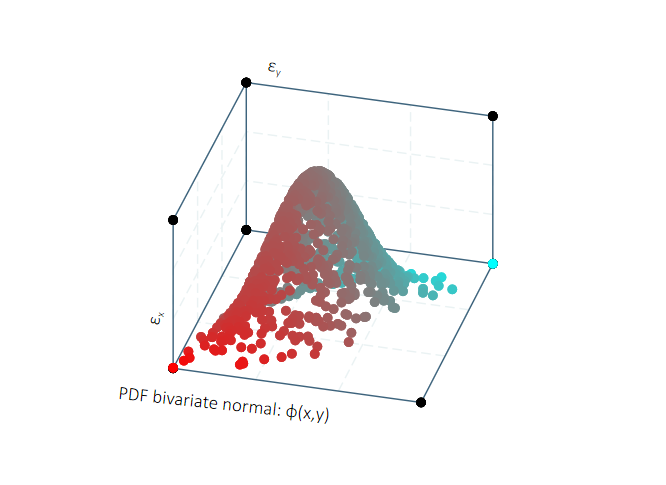
\includegraphics[width=0.49\textwidth]{figures/bivariate_normal_pdf}
		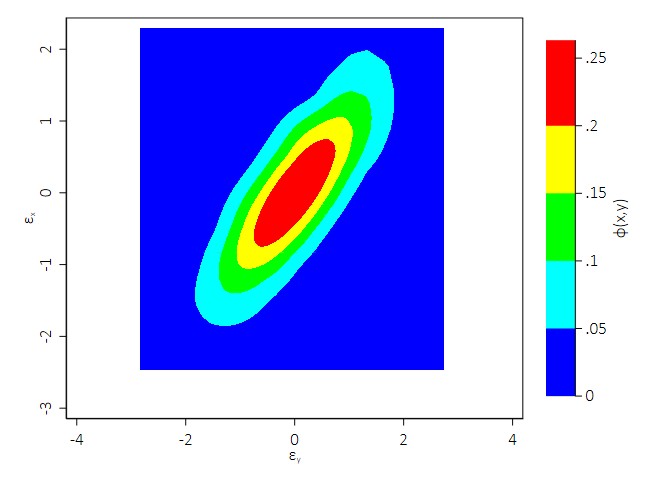
\includegraphics[width=0.49\textwidth]{figures/bivariate_normal_pdf_contour}
	\label{fig:bivariate_normal_pdf}\vspace{-25pt}
\end{figure}

\subsection{The joint cumulative density function}

\definitionbox{The joint cumulative density function.}{

The probability of a joint event of $X$ and $Y$ have $\textbf{joint cumulative density function}$
\begin{itemize}
	\item if $x$ and $y$ are discrete
$$F(x, y) =Prob(X \leq x, Y \leq y) = \sum_{X\leq x}\sum_{Y\leq y}f(x, y)$$
	\item if $x$ and $y$ are continuous
$$F(x, y) =Prob(X \leq x, Y \leq y)  = \int_{-\infty}^{x}\int_{-\infty}^{y}f(t, s)dsdt$$

\end{itemize}}

\examplebox{Example}{


With $x=2,y=2$ and the following $f(x,y)$


\noindent\begin{minipage}{\textwidth}
\begin{minipage}[c][6cm][c]{0.5\textwidth}
%-------------------------------------------
%\begin{landscape}

	
		\begin{table}[H]
%\caption{Timeline of German Reforms}
\label{tab:timeline}

		\begin{tabular}{lrr}
\toprule
$f(x,y)$ &$f(x,y=1)$ &$f(x,y=2)$      \\
\midrule
$f(x=1,y)$ &\cellcolor{lightblue}1/10  &\cellcolor{lightblue}2/10                                                                 \\
$f(x=2,y)$ &\cellcolor{lightblue}1/10  &\cellcolor{lightblue}2/10                                                              \\
$f(x=3,y)$   &0     &4/10                                                             \\
\bottomrule
		\end{tabular}
		%\begin{tablenotes}
			%\item \emph{Notes:}  the historical development of the regulatory measures. The lower part provides the most important regulatory changes and announcements within our observation period. \newline
%\emph{Sources:} Own description.
		%\end{tablenotes}
	\end{table}


%\end{landscape}
%-------------------------------------------

$Prob(X \leq 2 , Y \leq 2)=f(x=1, y=1)+$\\$f(x=2, y=1)+f(x=1, y=2)+f(x=2, y=2)=3/5.$

\end{minipage}\hfill
\begin{minipage}{0.5\textwidth}
	\centering
		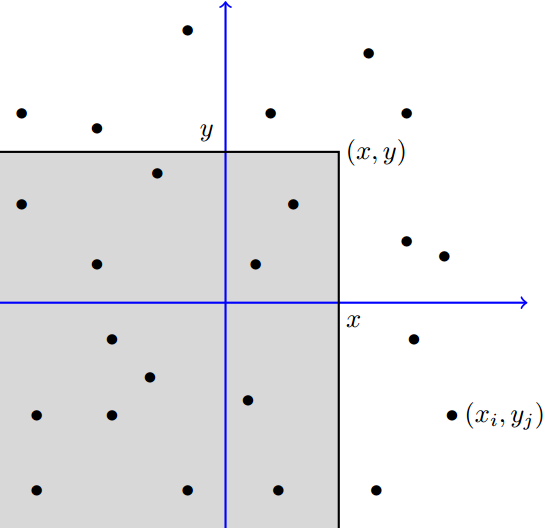
\includegraphics[width=.8\textwidth]{figures/jointcdf}
	\label{fig:jointcdf}
\end{minipage}
\end{minipage}
}




\definitionbox{Cumulative probability distribution}{
For values $x$ and $y$ of two discrete random variable $X$ and $Y$, the \textbf{cumulative probability distribution}
$$F(x,y)=Prob(X\leq x,Y\leq y).$$}

The axioms of probability require
$$0\leq F(x,y)\leq1,$$
$$F(\infty,\infty)=1,$$
$$F(-\infty,y)=0,$$
$$F(x,-\infty)=0.$$
The marginal probabilities can be found from the joint cdf
$$f_x(x)=P(X\leq x)=Prob(X\leq x,Y\leq \infty)=F(x,\infty).$$



\subsection{The marginal probability density}
\definitionbox{The marginal probability density}{
To obtain the marginal distributions $f_x(x)$ and $f_y(y)$ from the joint density $f(x,y)$, it is necessary to sum or integrate out the other variable.
For example,
\begin{itemize}
	\item if $x$ and $y$ are discrete
$$f_{x}(x)=\sum_{y}f(x, y),$$
	\item if $x$ and $y$ are continuous
$$f_{x}(x)=\int_{y}f(x, s)ds.$$
\end{itemize}}

\examplebox{Example}{
%-------------------------------------------
%\begin{landscape}

	\begin{center}
		\begin{threeparttable}[htbp]
%\caption{Timeline of German Reforms}
\label{tab:timeline}

		\begin{tabular}{lrrr}
\toprule
$f(x,y)$ &$f(x,y=1)$ &$f(x,y=2)$ & $f_x(x)$     \\
\midrule
$f(x=1,y)$ &\cellcolor{lightblue}1/10  &\cellcolor{lightblue}2/10          &\cellcolor{lightblue}\Circled[outer color=red1, inner ysep=3pt]{3/10}                                                          \\
$f(x=2,y)$ &1/10  &2/10          &3/10                                                       \\
$f(x=3,y)$   &0     &4/10        &4/10                                                        \\
$f_y(y)$    &2/10  &8/10 &1\\
\bottomrule
		\end{tabular}
		%\begin{tablenotes}
			%\item \emph{Notes:}  the historical development of the regulatory measures. The lower part provides the most important regulatory changes and announcements within our observation period. \newline
%\emph{Sources:} Own description.
		%\end{tablenotes}
	\end{threeparttable}
\end{center}

%\end{landscape}
%-------------------------------------------

$$f_x(x=1)=f(x=1,y=1)+f(x=1,y=2)=3/10.$$
$$f_y(y=2)=f(x=1,y=2)+f(x=2,y=2)+f(x=3,y=2)=4/5.$$
}





\subsubsection*{The bivariate normal distribution}
\begin{figure}[H]
	\centering
		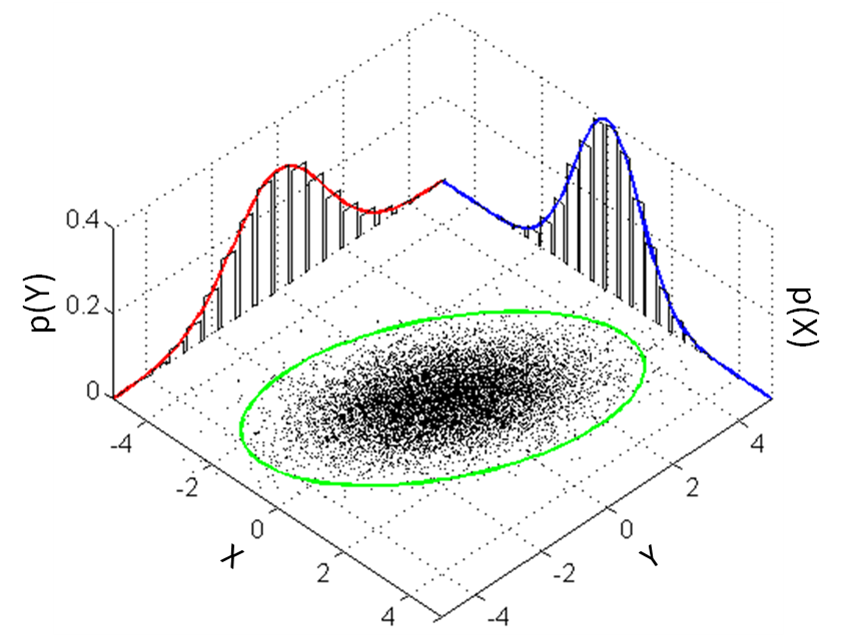
\includegraphics[width=0.90\textwidth]{figures/MultivariateNormal}
	\label{fig:MultivariateNormal}
\end{figure}




\subsubsection*{Why do we care about marginal distributions?}

Means, variances, and higher moments of the variables in a joint distribution are defined with respect to the marginal distributions.

\begin{itemize}
	\item \textbf{Expectations}\\
	If $x$ and $y$ are discrete
$$E[x] = \sum_{x}x f_{x}(x) =\sum_{x}x\left[\sum_{y}f(x, y)\right] = \sum_{x}\sum_{y} x f(x, y).$$
	If $x$ and $y$ are continuous
$$E[x] = \int_{x}x f_{x}(x) = \int_{x}\int_{y} x f(x, y)dydx.$$
	\item \textbf{Variances}
$$  Var[x] = \sum_{x}(x-E[x])^{2} f_{x}(x) = \sum_{x}\sum_{y} (x-E[x])^{2} f(x, y).$$

\end{itemize}



\subsection{Covariance and correlation}

 For any function $g(x, y)$,
\begin{equation*} E[g(x, y)]=\left\{
 \begin{array}{ll}
 {\sum_{x}\sum_{y}g(x, y)f(x, y)~~~~~~~~~ in~ the~ discrete~case, } \\
 {~}\\
 {\int_{x}\int_{y}g(x, y)f(x, x)dydx~~~~~~~ in~ the~ continuous~case.}
 \end{array}
 \right.
\end{equation*}
The covariance of $x$ and $y$ is a special case:
\begin{eqnarray*}
% \nonumber to remove numbering (before each equation)
  Cov[x, y] &=& E[(x - \mu_{x})(y - \mu_{y})] \\
  ~ &=& E[xy] - \mu_{x}\mu_{y} = \sigma_{xy}
\end{eqnarray*}
If $x$ and $y$ are independent, then $f(x, y) = f_{x}(x) f_{y}(y)$ and
\begin{eqnarray*}
% \nonumber to remove numbering (before each equation)
  \sigma_{xy} &=& \sum_{x}\sum_{y}f_{x}(x)f_{y}(y)(x-\mu_{x})(y-\mu_{y}) \\
  ~ &=& \sum_{x}(x-\mu_{x})f_{x}(x)\sum_{y}(y-\mu_{y})f_{y}(y) = E[x-\mu_{x}]E[y-\mu_{y}]= 0.
\end{eqnarray*}

\begin{itemize}
	\item correlation $\rho_{xy}=\frac{\sigma_{xy}}{\sigma_{x}\sigma_{y}}$
  \item $\sigma_{xy}=0$ does not imply independence (except for bivariate normal).
\end{itemize}




\definitionbox{Independence: Pdf and cdf from marginal densities}{


\begin{itemize}
	\item Two random variables are statistically independent if and only if their joint density is the product of the marginal densities:
$$f(x, y) = f_{x}(x) f_{y}(y) \Leftrightarrow x~ and~ y~ are~ independent.$$
	\item If (and only if) $x$ and $y$ are independent, then the marginal cdfs factors the cdf as well:
$$F(x, y) = F_{x}(x)F_{y}(y)=Prob(X \leq x, Y \leq y) = Prob(X \leq x)Prob(Y \leq y).$$
\end{itemize}}

\examplebox{Example}{
\begin{minipage}[t]{.52\textwidth}


%-------------------------------------------
%\begin{landscape}


		\begin{threeparttable}[htbp]
%\caption{Timeline of German Reforms}
\label{tab:timeline}

		\begin{tabular}{lrrr}
\toprule
$f(x,y)$ &$f(x,y=1)$ &$f(x,y=2)$ & $f_x(x)$     \\
\midrule
$f(x=1,y)$ &1/6  &1/6          &1/3                                                          \\
$f(x=2,y)$ &1/6  &1/6          &1/3                                                       \\
$f(x=3,y)$ &1/6  &\Circled[outer color=red1, inner ysep=3pt]{1/6}          &\cellcolor{lightblue}1/3                                                        \\
$f_y(y)$   &1/2  &\cellcolor{lightblue}1/2 &1\\
\bottomrule
		\end{tabular}
		%\begin{tablenotes}
			%\item \emph{Notes:}  the historical development of the regulatory measures. The lower part provides the most important regulatory changes and announcements within our observation period. \newline
%\emph{Sources:} Own description.
		%\end{tablenotes}
	\end{threeparttable}


%\end{landscape}
%-------------------------------------------

$$f_x(x=3)\times f_y(y=2)=1/3\times 1/2=1/6.$$

\end{minipage}\quad
\begin{minipage}[t]{0.48\textwidth}

%-------------------------------------------
%\begin{landscape}


		\begin{threeparttable}[htbp]
%\caption{Timeline of German Reforms}
\label{tab:timeline}

		\begin{tabular}{lrrr}
\toprule
$F(x,y)$ &$F(x,y=1)$ &$F(x,y=2)$      \\
\midrule
$F(x=1,y)$ &1/6  &\cellcolor{lightblue}2/6                                                                  \\
$F(x=2,y)$ &\cellcolor{lightblue}2/6  &4/6                                                               \\
$F(x=3,y)$ &3/6  &1                                                                  \\
\bottomrule
		\end{tabular}
		%\begin{tablenotes}
			%\item \emph{Notes:}  the historical development of the regulatory measures. The lower part provides the most important regulatory changes and announcements within our observation period. \newline
%\emph{Sources:} Own description.
		%\end{tablenotes}
	\end{threeparttable}

%\end{landscape}
%-------------------------------------------

$$\begin{aligned}&P(x\leq2)P(y\leq2)\\ &=[f(x=2,y=1) +f(x=2,y=2)]\\ &\times [f(x=1,y=2)+f(x=2,y=2)]\\
&=[1/6+1/6][1/6+1/6]=4/36=2/18.\end{aligned}$$

\end{minipage}%


}




\subsection{The conditional density function}
\definitionbox{The conditional density function}{

The $\textbf{conditional distribution}$ over $y$ for each value of $x$ (and vice versa) has
conditional densities
 $$f(y | x) = \frac{f(x, y)}{f_{x}(x)} \quad	 f(x | y) = \frac{f(x, y)}{f_{y}(y)}.$$}

The marginal distribution of $x$ averages the probability of $x$ given $y$ over the distribution of all values of $y$
$f_x(x)=E[f(x|y)f(y)].$ If $x$ and $y$ are independent, knowing the value of $y$ does not provide any information about $x$, so $f_x(x)=f(x|y).$\\

\examplebox{Example}{

%-------------------------------------------
%\begin{landscape}
		\begin{threeparttable}[htbp]
%\caption{Timeline of German Reforms}
\label{tab:timeline}

		\resizebox{\textwidth}{!}{\begin{tabular}{l@{\extracolsep{-2mm}}rrrr@{\extracolsep{0pt}}l@{\extracolsep{-2mm}}rrr}
\cmidrule(r){1-4}\cmidrule(r){6-9}
cond. distr.  &  & &  &	 &	joint distr.  &  &  &marginal pr.     \\
 $f(x|y)$ &$f(x|y=1)$ &$f(x|y=2)$ &$f(x|y=1,y=2)$ & &	$f(x,y)$ &$f(x,y=1)$ &$f(x,y=2)$  &  $f_x(x)$    \\
\cmidrule(r){1-4}\cmidrule(r){6-9}
$x=1$ &1/2  &1/4 &3/10 & &	$f(x=1,y)$ &1/10  &2/10 &3/10                                                                \\
$x=2$ &1/2  &1/4 &3/10 & &	$f(x=2,y)$ &1/10  &2/10 &3/10                                                             \\
$x=3$ &0  &\Circled[outer color=red1, inner ysep=3pt]{1/2} &4/10 & &	$f(x=3,y)$   &0     &\cellcolor{lightblue}4/10 &4/10                                                             \\
$\sum_x $ &1 &1  &1 &	& marginal pr. $f_y(y)$    &2/10  &\cellcolor{lightblue}8/10 &1                                            \\
\cmidrule(r){1-4}\cmidrule(r){6-9}
\end{tabular}}
		%\begin{tablenotes}
			%\item \emph{Notes:}  the historical development of the regulatory measures. The lower part provides the most important regulatory changes and announcements within our observation period. \newline
%\emph{Sources:} Own description.
		%\end{tablenotes}
	\end{threeparttable}
}

\bbox{
$$f(x=3|y=2)=\frac{f(x=3,y=2)}{f_y(y=2)}=4/10\times 10/8=1/2.$$
$$f_x(x=2)=E_y[f(x=2|y)f(y)]=f(x=2|y=1)f(y=1)+f(x=2|y=2)f(y=2)$$
$$=1/2\times2/10+1/4\times8/10=1/10+2/10=3/10.$$
}



\subsection{Conditional mean aka regression}


A random variable may always be written as
\begin{eqnarray*}
% \nonumber to remove numbering (before each equation)
  y &=& E[y | x] + (y - E[y | x]) \\
  ~ &=& E[y | x] + \epsilon.
\end{eqnarray*}


\definitionbox{Definition}{
The regression of $y$ on $x$ is obtained from the $\textbf{conditional mean}$
\begin{equation} E[y | x]=\left\{
 \begin{array}{ll}
 {\sum_{y}yf(y | x) ~~~~~~~ if~ y~ is~ discrete,}\\
 {~}\\
 {\int_{y}yf(y | x)dy~~~~~~~ if ~y~is~ continuous.}
 \end{array}
 \right.\nonumber
\end{equation}
}






Predict $y$ at values of $x$: $$\sum_{y}yf(y | x=1)=1\times 1/3+2\times 2/3=5/3.$$

\begin{figure}
	\centering
		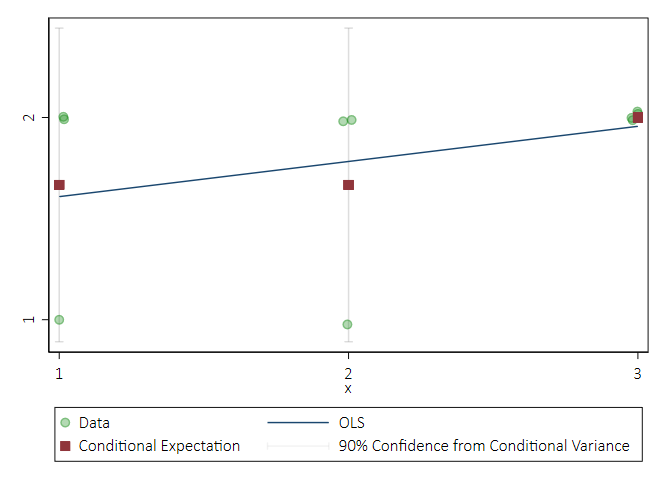
\includegraphics[width=0.90\textwidth]{figures/conditional_expectation}
	\label{fig:conditional_expectation}
\end{figure}





\definitionbox{Conditional variance}{

A $\textbf{conditional variance}$ is the variance of the conditional distribution:
{{\begin{equation} Var[y | x] =\left\{
 \begin{array}{ll}
 {\sum_{y}\left(y - E[y | x]\right)^{2}f(y | x) ~~~~~~~ if~ y~ is~ discrete,} \\
 {~}\\
 {\int_{y}\left(y - E[y | x]\right)^{2}f(y | x) dy,~~~~~ if ~y~is~ continuous. }
 \end{array}
 \right.\nonumber
\end{equation}}}
The computation can be simplified by using
\begin{equation}
    Var[y | x] = E[y^{2} | x] - \left(E[y | x]\right)^{2}\geq0.\nonumber
\end{equation}
Decomposition of variance $Var[y] = E_{x}[Var[y | x]]+Var_{x}[E[y | x]]$}
\begin{itemize}
	\item When we condition on $x$, the variance of $y$ reduces on average. $Var[y]\geq E_{x}[Var[y | x]]$
	\item $E_{x}[Var[y | x]]$ is the average of variances \textbf{within} each $x$
	\item $Var_{x}[E[y | x]]$ is variance \textbf{between} $y$ averages in each $x$.
	\item $E[y|x=1]=1.67$, $E[y|x=2]=1.67$, and $E[y|x=3]=2$
	\item $V[y|x=1]=0.22$, $V[y|x=2]=0.22$, and $V[y|x=3]=0$
\end{itemize}

\examplebox{Example}{



\begin{minipage}[t]{0.4\textwidth}


%-------------------------------------------
%\begin{landscape}

	
		\begin{threeparttable}[htbp]
%\caption{Timeline of German Reforms}
\label{tab:timeline}

		\begin{tabular}{lrrr}
\toprule
$f(y|x)$ &$y=1$ &$y=2$      \\
\midrule
$f(y|x=1)$ &1/3  &2/3          &1                                                          \\
$f(y|x=2)$ &1/3  &2/3          &1                                                       \\
$f(y|x=3)$ & 0  &1           &1                                                       \\
\bottomrule
		\end{tabular}
		%\begin{tablenotes}
			%\item \emph{Notes:}  the historical development of the regulatory measures. The lower part provides the most important regulatory changes and announcements within our observation period. \newline
%\emph{Sources:} Own description.
		%\end{tablenotes}
	\end{threeparttable}


%\end{landscape}
%-------------------------------------------

$$E[y|x=1]=1/3\times1+2/3\times 2=5/3$$
$$E[y|x=2]=1/3\times1+2/3\times 2=5/3$$
$$E[y|x=3]=0\times1+1\times 2=2$$

\end{minipage}\quad
\begin{minipage}[t]{.49\textwidth}

%-------------------------------------------
%\begin{landscape}


		\begin{threeparttable}[htbp]
%\caption{Timeline of German Reforms}
\label{tab:timeline}

		\begin{tabular}{lrrr}
\toprule
$f(x,y)$ &$f(x,y=1)$ &$f(x,y=2)$ & $f_x(x)$     \\
\midrule
$f(x=1,y)$ &1/10  &2/10 & 3/10                                                                 \\
$f(x=2,y)$ &1/10  &2/10 & 3/10                                                               \\
$f(x=3,y)$ &0     &4/10 & 4/10                                                       \\
$f_y(y)$   &2/10  &8/10 & 1                                                                \\
\bottomrule
		\end{tabular}
		%\begin{tablenotes}
			%\item \emph{Notes:}  the historical development of the regulatory measures. The lower part provides the most important regulatory changes and announcements within our observation period. \newline
%\emph{Sources:} Own description.
		%\end{tablenotes}
	\end{threeparttable}


%\end{landscape}
%-------------------------------------------

$$\begin{aligned}&V[y|x=1]=1^2\times 1/3+2^2\times 2/3-(5/3)^2=2/9\\
&V[y|x=2]=1^2\times 1/3+2^2\times 2/3-(5/3)^2=2/9 \\
&V[y|x=3]=1^2\times 0+2^2\times 1-2^2=0\end{aligned}$$

alternatively (requiring more differences)

$$V[y|x=1]=(1-5/3)^2\times 1/3+(2-5/3)^2\times 2/3=2/9$$

\end{minipage}%


}

Average of variances \textbf{within} each $x$, $E[V[y|x]]$ is less or equal total variance $V[y]$.\\

\examplebox{Example}{


\begin{itemize}
	\item Use the conditional mean to calculate $E[y]$:
$$E[y]=E_x[E[y|x]]=E[y|x=1]f(x=1)+E[y|x=2]f(x=2)+E[y|x=3]f(x=3)$$$$=5/3\times 3/10+5/3\times 3/10+2\times 4/10=9/5.$$
$$E[y]=\sum_yf_y(y)=1\times 2/10+2\times 8/10=9/5.$$
	\item Variation in $y$, $V[y|x=1]=0.22$, $V[y|x=2]=0.22$, and $V[y|x=3]=0$ due to variation in $x$, is on average\\ $E[V[y|x]]=3/10\times2/9+3/10\times2/9+4/10\times0=2/15.$
    \item For each conditional mean $E[y|x=1]=5/3$, $E[y|x=2]=5/3$, and $E[y|x=3]=2$, $y$ varies with\\
	$V[E[y|x]]=E[(E[y|x])^2]-(E[y|x])^2=3/10\times(5/3)^2+3/10\times(5/3)^2+4/10\times(2)^2-(9/5)^2=2/75.$
    \end{itemize}}
    \bbox{
    \begin{itemize}
	\item $E[V[y|x]]+V[E[y|x]]=V[y]=2/75+2/15=4/25.$\\
With degree of freedom correction $(n-1)$ (as reported in software):\\
$E[V[y|x]]+V[E[y|x]]=V[y]=2/75/(10-1)\times 10+2/15/(10-1)\times 10=8/45.$
\end{itemize}


}



\subsection{The bivariate normal}
\subsubsection*{Properties of the bivariate normal}


Recall bivariate normal distribution is the joint distribution of two normally distributed variables. The density is
\begin{equation*}
    f(x, y) =\frac{1}{2\pi\sigma_{x}\sigma_{y}\sqrt{1 - \rho^{2}}}e^{-1/2[(\epsilon^{2}_{x}+\epsilon^{2}_{y}-2\rho \epsilon_{x} \epsilon_{y})/(1-\rho^{2})],}
\end{equation*}
where $\epsilon_{x} = \frac{x - \mu_{x}}{\sigma_{x}},$ and $\epsilon_{y} = \frac{y - \mu_{y}}{\sigma_{y}}.$

The covariance is $\sigma_{xy}=\rho_{xy}\sigma_{x}\sigma_{y},$ where
\begin{itemize}
	\item $-1<\rho_{xy}<1$ is the correlation between $x$ and $y$
	\item $\mu_x,\sigma_{x},\mu_y,\sigma_{y}$ are means and standard deviations of the marginal distributions of $x$ or $y$
\end{itemize}




If $x$ and $y$ are bivariately normally distributed $(x,y)\sim N_2[\mu_x,\mu_y,\sigma^2_{x},\sigma^2_{y},\rho_{xy}]$
\begin{itemize}
	\item the marginal distributions are normal $$f_x(x)=N[\mu_x,\sigma_x^2]$$$$f_y(y)=N[\mu_y,\sigma_y^2]$$
	\item the conditional distributions are normal $$f(y|x)=N[\alpha + \beta x, \sigma_y^2(1-\rho^2)]$$ $$\alpha=\mu_y-\beta \mu_x; \beta=\frac{\sigma_{xy}}{\sigma^2_{x}}$$
	\item $f(x,y)=f_x(x)f_x(x)$ if $\rho_{xy}=0$: $x$ and $y$ are independent if and only if they are uncorrelated
\end{itemize}


\subsection{Useful rules}


\begin{itemize}
	\item $\rho_{xy}=\frac{\sigma_{xy}}{\sigma_{x}\sigma_{y}}$
	\item $E[ax + by + c] = aE[x] + bE[y] + c$
	\item $Var[ax + by + c] = a^{2}Var[x] + b^{2}Var[y] + 2abCov[x, y]=Var[ax + by]$
	\item $Cov[ax + by, cx + dy] = ac Var[x] + bd Var[y] + (ad + bc)Cov[x, y]$
	\item If $X$ and $Y$ are uncorrelated, then $Var[x + y] = Var[x - y] = Var[x] + Var[y].$
	\item Linearity
	$$E[ax + by |z] = aE[x|z] + bE[y|z].$$
	\item Adam's Law / Law of Iterated Expectation
	$$E[y] = E_{x}[E[y | x]]$$
	\item Adam's general Law / Law of Iterated Expectation
	$$E[y|g_{2}(g_{1}(x))] = E[E[y | g_{1}(x)]|g_{2}(g_{1}(x))]$$
	\item Independence\\
	If $x$ and $y$ are independent, then $$E[y] = E[y|x],$$
	$$E[g_{1}(x)g_{2}(y)] = E[g_{1}(x)]E[g_{2}(y)].$$
	\item Taking out what is known
	$$E[g_{1}(x)g_{2}(y)|x] = g_{1}(x)E[g_{2}(y)|x].$$
	\item Projection of $y$ by $E[y|x]$, such that orthogonal to $h(x)$
	$$E[(y-E[y|x])h(x)] = 0.$$
	\item Keeping just what is needed ($y$ predictable from $x$ needed, not residual)
	$$E[xy] = E[xE[y|x]].$$
	\item Eve's Law (EVVE) / Law of Total Variance
	$$Var[y] = E_{x}[Var[y | x]] + Var_{x}[E[y | x]]$$
	\item ECCE law / Law of Total Covariance
	$$Cov[x,y] = E_{z}[Cov[y,x | z]] + Cov_{z}[E[x | z],E[y | z]]$$
	\item $Cov[x, y] = Cov_{x}[x, E[y | x]] =\int_{x}\left(x - E[x]\right)E[y | x] f_{x}(x) dx.$
	\item If $E[y | x] = \alpha + \beta x$, then $\alpha = E[y] - \beta E[x]$ and $\beta= \frac{Cov[x, y]}{Var[x]}$
	\item Regression variance $Var_{x}[E[y | x]]$, because $E[y | x]$ varies with $x$
	\item Residual variance $E_{x}[Var[y | x]] = Var[y] - Var_{x}[E[y | x]]$, because $y$ varies around the conditional mean
	\item Decomposition of variance $Var[y] = Var_{x}[E[y | x]] + E_{x}[Var[y | x]]$
	\item Coefficient of determination $= \frac{\text{regression~ variance}}{\text{total variance}}$
	\item If $E[y | x] = \alpha + \beta x$ and if $Var[y | x]$ is a constant, then $$Var[y | x] = Var[y]\left(1 - Corr^{2}[y, x]\right)= \sigma^{2}_{y}\left(1 - \sigma^{2}_{xy}\right)$$
\end{itemize}





\clearpage
\section{The Least Squares Estimator}
\label{The Least Squares Estimator}

\subsection{What is the Relationship between Two Variables?}



\subsubsection*{Political Connections and Firms}

Firm profits increase with the degree of political connections

\begin{figure}[H]
	\centering
		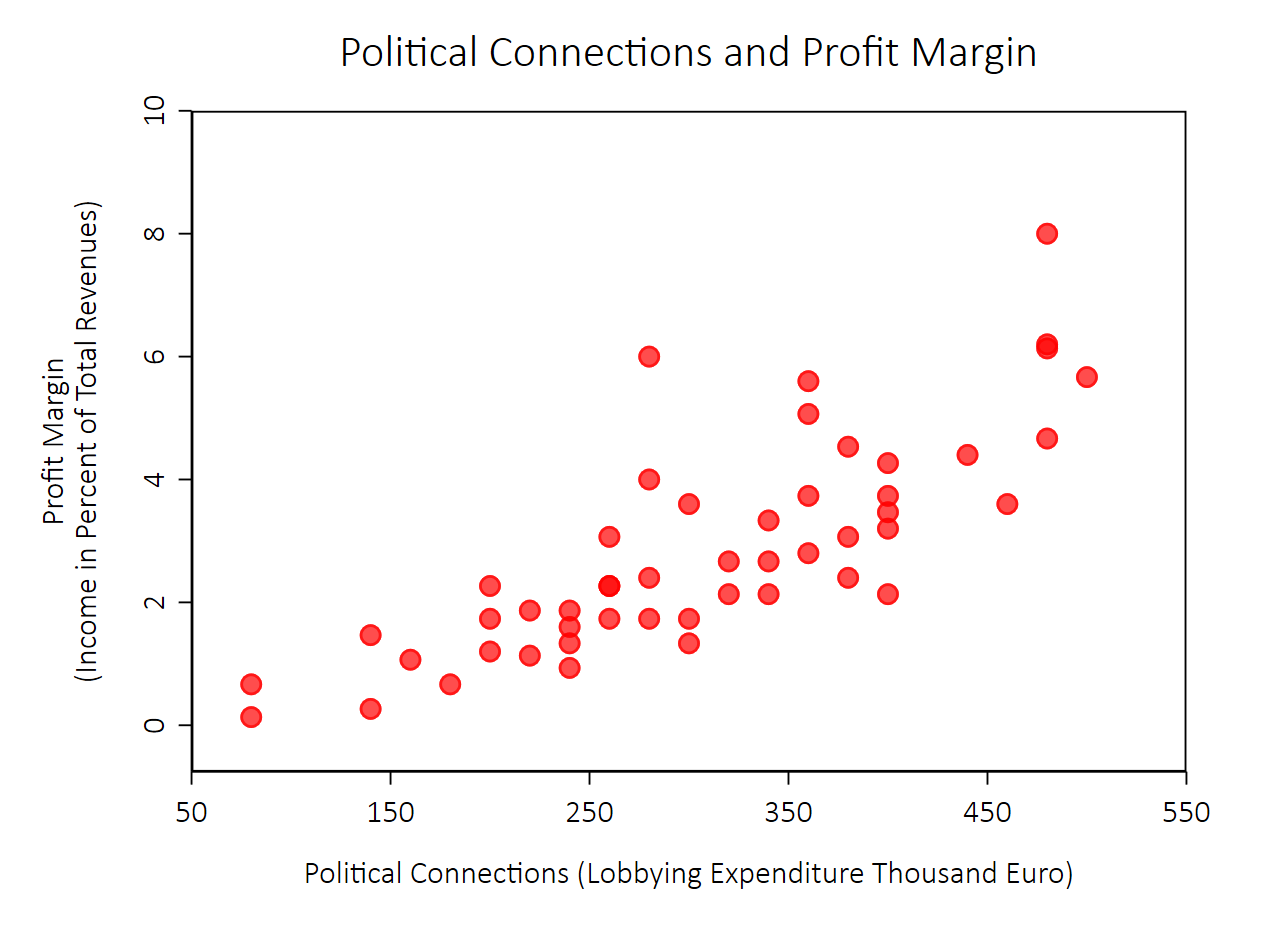
\includegraphics[width=.9\textwidth]{figures/politicallyconnected1}
   \label{fig:politicallyconnected1}
\end{figure}

\begin{itemize}
	\item Learn how to represent relationships between two or more variables
	\item How to quantify and predict effects of shocks and policy changes
	\item Show properties of the OLS estimator in small \& large samples
	\item Apply Monte Carlo Simulations to assess properties of OLS

\end{itemize}

\clearpage
\subsection{The Econometric Model}


\subsubsection*{Specification of a Linear Regression}
%



    \begin{itemize}
        \item dependent variable $y_i = $ profits of firm $i$
        \item explanatory variables $x_{i1}, \ldots, x_{iK}$ $k=1,\ldots K$ political connections, other firm characteristics
        \item $x_{i0} = 1$ is a constant
        \item parameters to be estimated $\beta_0, \beta_1, \ldots, \beta_K$ are $K+1$
        \item $u_i$ is called the error term
    \end{itemize}


        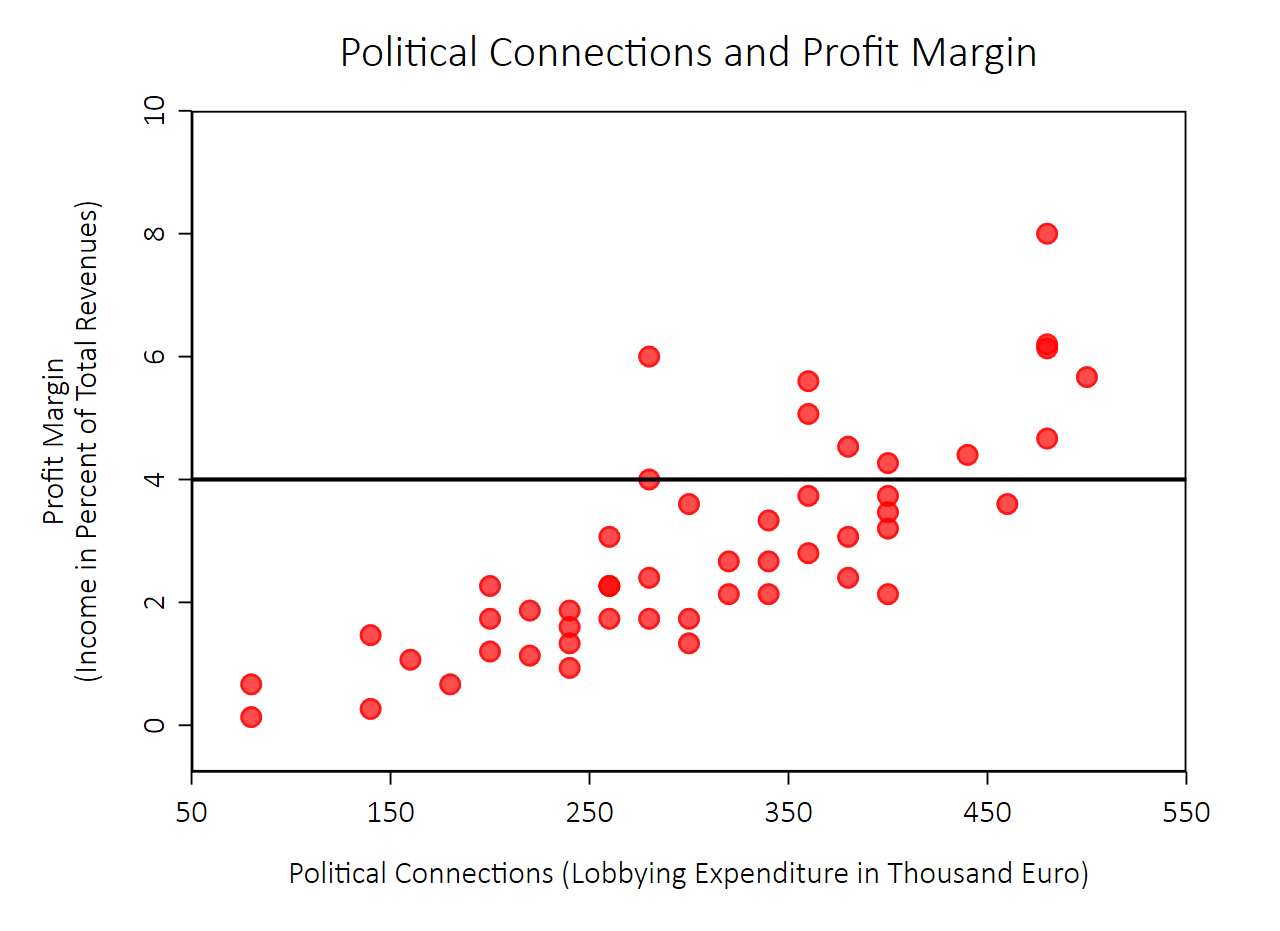
\includegraphics[width=.9\textwidth]{figures/politicallyconnected2}

  % End two-column layout

$$y_i = (\beta_0=4) + (\beta_1=0) x_{i1} + u_{i}.$$\vspace{5pt}



    \begin{itemize}
        \item dependent variable $y_i = $ profits of firm $i$
        \item explanatory variables $x_{i1}, \ldots, x_{iK}$ $k=1,\ldots K$ political connections, other firm characteristics
        \item $x_{i0} = 1$ is a constant
        \item parameters to be estimated $\beta_0, \beta_1, \ldots, \beta_K$ are $K+1$
        \item $u_i$ is called the error term
    \end{itemize}


        \includegraphics[width=.9\textwidth]{figures/politicallyconnected3}


$$y_i = (\beta_0=2.36) + (\beta_1=0.01) x_{i1} + u_{i}.$$




\subsubsection*{How Were the Data Generated?}

The \emph{data generating process} is fully described by a set of assumptions.\\[2ex]
\textbf{The Five Assumptions of the Econometric Model}
\begin{itemize}
	\item LRM1: Linearity
	\item LRM2: Simple random sampling
	\item LRM3: Exogeneity
	\item LRM4: Error variance
	\item LRM5: Identifiability
\end{itemize}



\newpage
\subsubsection*{Data Generating Process: Linearity}
%

\definitionbox{LRM1: Linearity}{
$$y_i = \beta_0 + \beta_1 x_{i1} + \ldots + \beta_K x_{iK} + u_{i} \text{ and } E(u_i)=0.$$
}
LRM1 assumes that the
\begin{itemize}
	\item functional relationship is linear in parameters $\beta_k$
	\item error term $u_{i}$ enters additively
	\item parameters $\beta_k$ are constant across individual firms $i$ and $j\neq i$.
\end{itemize}




\subsubsection*{Anscombe's Quartet}
%

%-------------------------------------------
%\begin{landscape}
%\begin{figure*}
\begin{figure}[H]
	\begin{subfigure}[c]{0.49\textwidth}
 \centering
\includegraphics[width=1\textwidth]{figures/Anscombe_data1}
 						
  \end{subfigure}%
	\begin{subfigure}[c]{0.49\textwidth}
 \centering
\includegraphics[width=1\textwidth]{figures/Anscombe_data2}
							
  \end{subfigure}\\
		\begin{subfigure}[c]{0.49\textwidth}
 \centering
\includegraphics[width=1\textwidth]{figures/Anscombe_data3}
					
  \end{subfigure}%
	\begin{subfigure}[c]{0.49\textwidth}
 \centering
\includegraphics[width=1\textwidth]{figures/Anscombe_data4}
							
  \end{subfigure}
 	\caption{ All four sets are identical when examined using linear statistics, but very different when graphed. Correlation between x and y is 0.816. Linear Regression y = 3.00 + 0.50x.}

\end{figure}
%\end{figure*}
%\end{landscape}
%-------------------------------------------


\newpage
\subsubsection*{Data Generating Process: Random Sampling}
%

\definitionbox{LRM2: Simple Random Sampling}{
$$\{x_{i1},\ldots, x_{iK}, y_i\}^N_{i=1} \quad\text{i.i.d. (independent and identically distributed)}$$}
LRM2 means that
\begin{itemize}
	\item observation $i$ has no information content for observation $j\neq i$
	\item all observations $i$ come from the same distribution
\end{itemize}
This assumption is guaranteed by simple random sampling provided there is no systematic non-response or truncation.





\subsubsection*{Density of Population and Truncated Sample}
\begin{figure}[H]
	\centering
    \includegraphics[width=.9\textwidth]{figures/Trunc1}

	\caption{ Distribution of a dependent variable and an independent variable truncated at $y^*=15$.\label{fig:LRM}}
\end{figure}



\newpage

\subsubsection*{Data Generating Process: Exogeneity}
%
\definitionbox{LRM3: Exogeneity}{
\begin{enumerate}
\item \hfill $u_{i}|x_{i1},\ldots, x_{iK} \sim N(0, \sigma^2_i)$\hfill\null

LRM3a assumes that the error term is normally distributed conditional on the explanatory variables.
\item \hfill$u_i\; \bot\; x_{ik} \quad \forall k\quad\text{(independent)}, pdf_{u,x}(u_{i}x_{ik})=pdf_{u}(u_{i})pdf_{x}(x_{ik})$ \hfill\null

LRM3b means that the error term is independent of the explanatory variables.
\item \hfill $E(u_{i}|x_{i1},\ldots, x_{iK})=E(u_{i})=0 \quad \text{(mean independent)}$\hfill\null

LRM3c states that the \emph{mean} of the error term is independent of explanatory variables.
\item \hfill $cov(x_{ik},u_i)=0 \quad \forall k\quad\text{(uncorrelated)}$\hfill\null

LRM3d means that the error term and the explanatory variables are uncorrelated.
\end{enumerate}
}
LRM3a or LRM3b imply LRM3c and LRM3d. LRM3c implies LRM3d.



%\subsubsection*{(Conditional) Mean Independence}
\begin{figure}[H]
	\centering
		\includegraphics[width=.9\textwidth]{figures/meanindependence_cut}
	\caption{ Distributions of the dependent variable conditional on values of an independent variable.\label{fig:LRM}}
\end{figure}

Weaker exogeneity assumption if interest only in, say, $x_{i1}$:\\
\textbf{Conditional Mean Independence} $E(u_{i}|x_{i1},x_{i2},\ldots, x_{iK})=E(u_{i}|x_{i2},\ldots, x_{iK})$\\
Given the control variables $x_{i2},\ldots, x_{iK}$, the mean of $u_i$ does not depend on the variable of interest $x_{i1}$.


\newpage
\subsubsection*{Data Generating Process: Error Variance}
%

 \definitionbox{LRM4: Error Variance}{
\begin{enumerate}
\item $$V(u_{i}|x_{i1},\ldots, x_{iK})=\sigma^2 < \infty \quad \text{(homoskedasticity)}$$
LRM4a means that the variance of the error term is a constant.
\item $$V(u_{i}|x_{i1},\ldots, x_{iK})=\sigma^2_{i} = g(x_{i1},\ldots, x_{iK}) < \infty \quad \text{(cond. heteroskedasticity)}$$
LRM4b allows the variance of the error term to depend on a function $g$ of the explanatory variables.
\end{enumerate}
}


\subsubsection*{Heteroskedasticity}

\begin{figure}[H]
	\centering
{		\includegraphics[width=.49\textwidth]{figures/homo}}
{		\includegraphics[width=.49\textwidth]{figures/hetero}}
	\caption{The simple regression model under homo- and heteroskedasticity. $Var(profits|lobbying, employees)$ increasing with $lobbying$.
	%\cite{Wooldridge2009}.\label{fig:homo}
	}
\end{figure}



\newpage
\subsubsection*{Data Generating Process: Identifiability}
%
\definitionbox{LRM5: Identifiability}{
$$(x_{i0},x_{i1},\ldots, x_{iK}) \text{ are not linearly dependent}$$
$$0 < V(x_{ik}) < \infty \quad \forall k>0$$
}

LRM5 assumes that
\begin{itemize}
	\item the regressors are not \emph{perfectly collinear}, i.e. no variable is a linear combination of the others
	\item all regressors (but the constant) have strictly positive variance both in expectations and in the sample and not too many extreme values.
\end{itemize}
LRM5 means that every explanatory variable adds additional information.


\subsubsection*{The Identifying Variation from $x_{ik}$}

\begin{figure}[H]
	\centering
		\includegraphics[width=.9\textwidth]{figures/identifiability}
	\caption{The number of red and blue dots is the same. Using which would you get a more accurate regression line? \label{fig:LRM}}
\end{figure}








\newpage
\subsection{Estimation with OLS}





\textbf{Ordinary least squares (OLS)} minimizes the squared distances (SD) between the observed and the predicted dependent variable $y$:
$$\min_{\beta_0,\ldots,\beta_K}{SD(\beta_0,\ldots,\beta_K)},$$
$$\text{where } SD=\sum^{N}_{i=1}{[y_i-(\beta_0+\beta_1x_{i1}+\ldots+\beta_Kx_{iK})]^2}.$$



\subsubsection*{How to Describe the Relationship Best?}
    \begin{center}
\includegraphics[width=.9\textwidth]{figures/OLS1}
     \end{center}

\clearpage


    \begin{center}
\includegraphics[width=.9\textwidth]{figures/OLS2}
     \end{center}



    \begin{center}
\includegraphics[width=.9\textwidth]{figures/OLS3}
     \end{center}



    \begin{center}
\includegraphics[width=.9\textwidth]{figures/OLS4}
     \end{center}




    \begin{center}
\includegraphics[width=.9\textwidth]{figures/OLS5}
     \end{center}


\clearpage


\subsubsection*{Invention of OLS}
%

\begin{multicols}{2}  % Start two-column layout

    Legendre to Jacobi (Paris, 30 November 1827, \citealp{Plackett1972}): ``\textit{...How can Mr. Gauss have dared to tell you that the greater part of your theorems were known to him...?}\\[1ex] \textit{ ... this is the same man ... who wanted to appropriate in 1809 the method of least squares published in 1805.}\\[2ex] \textit{--- Other examples will be found in other places, but a man of honour should refrain from imitating them.}''

    \columnbreak  % Force the content into the second column

    \begin{figure}[H]
        \centering
        \includegraphics[width=0.55\textwidth]{figures/Legendre}
        \caption{ Watercolor caricature of Legendre by Boilly (1820), the only existing portrait known.}
    \end{figure}

\end{multicols}  % End two-column layout



\subsubsection*{Invention of OLS}
%

\begin{multicols}{2}  % Start two-column layout

    Legendre to Jacobi (Paris, 30 November 1827, \citealp{Plackett1972}): ``\textit{...How can Mr. Gauss have dared to tell you that the greater part of your theorems were known to him...?}\\[1ex] \textit{ ... this is the same man ... who wanted to appropriate in 1809 the method of least squares published in 1805.}\\[2ex] \textit{--- Other examples will be found in other places, but a man of honour should refrain from imitating them.}''

    \columnbreak  % Force the content into the second column

    \begin{figure}[H]
        \centering
        \includegraphics[width=0.55\textwidth]{figures/Gauss_klein}
        \caption{ Portrait of Gauss by Jensen (1840).}
    \end{figure}

\end{multicols}  % End two-column layout



\subsubsection*{Estimation with OLS}

For the bivariate regression model, the OLS estimators of $\beta_0$ and $\beta_1$ are \\

$$\hat{\beta}_0=\bar{y}-\hat{\beta}_1\bar{x}$$
$$\hat{\beta}_1=\frac{\sum^{N}_{i=1}{(x_{i1}-\bar{x})(y_{i}-\bar{y})}}{\sum^{N}_{i=1}{(x_{i1}-\bar{x})^2}}=\frac{cov(x,y)}{var(x)}$$


$$\hat{\beta}_1=cov(x,y)/(s_xs_x)=Rs_y/s_x,$$
where $R\equiv cov(x,y)/(s_xs_y)$ is \textbf{Pearson's correlation coefficient} with $s_z$ denoting the standard deviation of $z$.

%That is, the slope coefficient is equal to the correlation coefficient $R$ times the ratio of standard deviations of $y$ and $x$.



\subsubsection*{OLS estimator Measures Linear Correlation}

Equivalently,
$$R=s_x/s_y \hat{\beta}_1= \frac{\hat{\beta}_1\sum^{N}_{i=1}{(x_{i1}-\bar{x}})}{\sum^{N}_{i=1}{(y_{i}-\bar{y})}}=\frac{\sum^{N}_{i=1}{(\hat{\beta}_1x_{i1}-\hat{\beta}_1\bar{x}})}{\sum^{N}_{i=1}{(y_{i}-\bar{y})}}.$$

Squaring gives
$$R^2 =\frac{\sum^{N}_{i=1}{(\hat{y}_{i}-\bar{y})^2}}{\sum^{N}_{i=1}{(y_{i}-\bar{y})^2}}=1 - \frac{\sum^{N}_{i=1}{\hat{u}^2_{i}}}{\sum^{N}_{i=1}{(y_{i}-\bar{y})^2}}.$$
$R^2$ as measure of the \textbf{goodness of fit}:\\The fit improves with the fraction of the sample variation in $y$ that is explained by the $x$.


\subsubsection*{The Case with $K$ Explanatory Variables}




    The more general case with $K$ explanatory variables is
    $$\underset{(K+1) \times 1}{\hat{\beta}}=\underset{(K+1) \times (K+1)}{(X'X)^{-1}}\;\underset{(K+1) \times N}{X'}\;\underset{N \times 1}{y}$$


Given the OLS estimator, we can predict the
\begin{itemize}
	\item dependent variable by $\hat{y_i} = \hat{\beta}_0 + \hat{\beta}_1x_{i1} + \ldots + \hat{\beta}_K x_{iK}$
	\item the error term by $\hat{u}_i = y_i - \hat{y}_i$.
\end{itemize}
  $\hat{u}_i$ is called the \emph{residual}.\\[2ex]

\textbf{Adjusted $R^2$} $= 1 - \frac{N-1}{N-K-1}\frac{\sum^{N}_{i=1}{\hat{u}^2_{i}}}{\sum^{N}_{i=1}{(y_{i}-\bar{y})^2}}.$


    \begin{figure}[H]
        \centering
        \includegraphics[width=0.8\textwidth]{figures/3d_cloud1}
        \caption{ Scatter cloud visualized with\\ \textcolor{red1}{GRAPH3D for Stata}.}
        \label{fig:LRM}
    \end{figure}
    \begin{figure}[H]
        \centering
        \includegraphics[width=0.8\textwidth]{figures/3d_cloud2}
        \caption{ OLS surface visualized with\\ \textcolor{red1}{GRAPH3D for Stata}.}
        \label{fig:LRM}
    \end{figure}





\subsection{Properties of the OLS Estimator in the Small and in the Large}



\subsubsection*{Properties of the OLS Estimator}



\begin{itemize}
	\item \emph{Small sample properties of $\hat{\beta}$}
\begin{itemize}
	\item unbiased
	\item normally distributed
	\item efficient\\[4ex]
\end{itemize}
	\item \emph{Large sample properties of $\hat{\beta}$}
\begin{itemize}
	\item consistent
	\item approx. normal
	\item asymptotically efficient
\end{itemize}
\end{itemize}



\clearpage


\subsection*{Small Sample Properties}
\begin{figure}[H]
	\centering
		\includegraphics[width=.9\textwidth]{figures/SmallSample_empty}
	\caption{What is a small sample?\hspace{\textwidth} \emph{Source:} Familien-Duell \hspace{\textwidth}Grundy Light Entertainment. \label{fig:SS}}
\end{figure}




\begin{figure}[H]
	\centering
		\includegraphics[width=.9\textwidth]{figures/SmallSample}
	\caption{What is a small sample? \cite[p. 755]{Wooldridge2009}: ``But large sample approximations have been known to work well for sample sizes as small as $N = 20$.''  \emph{Source:} Familien-Duell Grundy Light Entertainment. \label{fig:SS}}
\end{figure}


\subsubsection*{Unbiasedness and Normality of $\hat{\beta}_k$}

Assuming LRM1,  LRM2,  LRM3a,  LRM4, and  LRM5,\\  the following properties can be established even for small samples.
\begin{itemize}
\item The OLS estimator of $\beta$ is \textbf{unbiased}.\\
$$E(\hat{\beta}_k|x_{11},\ldots,x_{NK})=\beta_k.$$

\item The OLS estimator is (multivariate) \textbf{normally distributed}.\\
$$\hat{\beta}_k|x_{11},\ldots,x_{NK}\sim N(\beta_k,V(\hat{\beta}_k)).$$

\item Under homoskedasticity (LRM4a)\\ the variance $\widehat{V}(\hat{\beta}_k|x_{11},\ldots,x_{NK})$ can be \textbf{unbiasedly} estimated.
\end{itemize}


\subsubsection*{Variance of $\hat{\beta}_k$ and Efficiency}

\begin{itemize}
\item For the bivariate regression model, it is estimated as
$$\widehat{V}=\frac{\hat{\sigma}^2}{\sum^{N}_{i=1}{(x_i-\bar{x})^2}} \text{ with}$$
$$\hat{\sigma}^2=\frac{\sum^{N}_{i=1}{\hat{u}^2_i}}{N-K-1}.$$
\item Gau{\ss}-Markov-Theorem: under homoskedasticity (LRM4a)\\$\hat{\beta}_k$ is the \textbf{BLUE} (best linear unbiased estimator, e.g., non-linear least squares biased).
\item $\widehat{V}(\hat{\beta}_k)$ inflates with
\begin{itemize}
	\item \textbf{micronumerosity} (small sample size)
	\item \textbf{multicollinearity} (high (but not perfect) correlation between two or more of the independent variables).
\end{itemize}
\end{itemize}



\subsubsection*{Unbiasedness}

\begin{itemize}
\item The OLS estimator of $\beta$ is \emph{unbiased}.\\
Plug $y=X\beta+u$ into the formula for $\hat\beta$ and then use the law of iterated expectation to first take expectation with respect to $u$ conditional
on $X$ and then take the unconditional expectation:

$$\operatorname{E}[\,\hat\beta] = E_{X,u}\Big[(X'X)^{-1}X'(X\beta+u)\Big]$$
$$= \beta + E_{X,u}\Big[(X'X)^{-1}X'u\Big]$$
$$= \beta + E_{X}\Big[E_{u|X}\Big[(X'X)^{-1}X'u|X \Big]\Big] $$
$$= \beta + E_{X}\Big[(X'X)^{-1}X'E_{u|X}[u|X]\Big]$$
$$= \beta,$$

where $E[u|X]=0$ by assumptions of the model.
\end{itemize}



\subsubsection*{Variance}

\begin{itemize}
\item The OLS estimator $\beta$ has variance $\widehat{V}(\hat{\beta}_k|x_{11},\ldots,x_{NK}) = \sigma^2 (X'X)^{-1}$ \\
Let $\sigma^2 I$ denote the covariance matrix of $u$. Then,

$$E[\,(\hat\beta - \beta)(\hat\beta - \beta)'] = E\Big[ ((X'X)^{-1}X'u)((X'X)^{-1}X'u)' \Big] $$
$$= E\Big[ (X'X)^{-1}X'uu'X(X'X)^{-1} \Big] $$
$$= E\Big[ (X'X)^{-1}X'\sigma^2X(X'X)^{-1} \Big] $$
$$= E\Big[ \sigma^2(X'X)^{-1}X'X(X'X)^{-1} \Big] $$
$$= \sigma^2 (X'X)^{-1}, $$

where we used the fact that $\hat{\beta} - \beta $ is just an affine transformation of $u$ by the matrix $(X'X)^{-1}X'$.


\end{itemize}


\subsubsection*{Estimator for Variance}


For a simple linear regression model, where $\beta = [\beta_0,\beta_1]'$ ($\beta_0$ is the y-intercept and $\beta_1$ is the slope), one obtains

$$\sigma^2 (X'X)^{-1} =  \sigma^2 \left(\sum x_ix_i'\right)^{-1}$$
$$=  \sigma^2 \left(\sum (1,x_i)' (1,x_i) \right)^{-1}$$
$$=  \sigma^2 \left(\sum \begin{pmatrix} 1 x_i\\x_i x_i^2\end{pmatrix} \right)^{-1}$$
$$=  \sigma^2 \begin{pmatrix} N \sum x_i\\\sum x_i \sum x_i^2\end{pmatrix}^{-1}$$
$$=  \sigma^2 \cdot \frac{1}{N\sum x_i^2-(\sum x_i)^2}\begin{pmatrix} \sum x_i^2 -\sum x_i\\-\sum x_i N\end{pmatrix}$$
$$=  \sigma^2 \cdot \frac{1}{N\sum_{i=1}^N{(x_i - \bar{x})^2}}\begin{pmatrix} \sum x_i^2 -\sum x_i\\-\sum x_i N\end{pmatrix}$$
$$Var(\beta_1) = \frac{\sigma^2}{\sum_{i=1}^N{(x_i - \bar{x})^2}}.$$




\subsubsection*{Parameter Values for Simulations}



\textbf{Monte Carlo Simulations} show the distribution of the estimate.
Suppose the data generating process is
$$y_i = \beta_0 + \beta_1 x_{i1} + u_{i}.$$

\begin{multicols}{2}  % Start two-column layout

    \begin{itemize}
        \item $\beta_0 = 2.00$
        \item $\beta_1 = 0.5$
        \item $u_i \sim N(0.00, 1.00)$
        \item $N=3, N=5, N=10,$\\ $N=25, N=100, N=1000$
    \end{itemize}

    \columnbreak  % Force the content into the second column
\vspace*{1cm}
    Try it yourself...

\end{multicols}  % End two-column layout
\clearpage

\subsubsection*{How to Establish Asymptotic Properties of $\hat{\beta}_k$?}
%

    \textbf{Law of Large Numbers}\\
    As $N$ increases, the distribution of $\hat{\beta}_k$ becomes more tightly centered around $\beta_k$.

    \



    % Start figure with subfigures
    \begin{figure}[H]
        \begin{subfigure}[c]{0.49\textwidth}
            \centering
            \includegraphics[width=1\columnwidth]{figures/distribution_beta1_3}
            \caption{N=3}
            \label{fig:distribution beta1 N3}
        \end{subfigure}%
        \begin{subfigure}[c]{0.49\columnwidth}
            \centering
            \includegraphics[width=1\columnwidth]{figures/distribution_beta1_5}
            \caption{N=5}
            \label{fig:distribution beta1 N5}								
        \end{subfigure}\\

        \begin{subfigure}[c]{0.49\columnwidth}
            \centering
            \includegraphics[width=1\textwidth]{figures/distribution_beta1_10}
            \caption{N=10}
            \label{fig:distribution beta1 N10}								
        \end{subfigure}
        \begin{subfigure}[c]{0.49\columnwidth}
            \centering
            \includegraphics[width=1\columnwidth]{figures/distribution_beta1_100}
            \caption{N=100}
            \label{fig:distribution beta1 N100}								
        \end{subfigure}
    \end{figure}
    % End figure with subfigures






%

\
\newpage
    \textbf{Central Limit Theorem}\\
    As $N$ increases, the distribution of $\hat{\beta}_k$ becomes normal (starting from a $t$-distribution).

\


    % Start figure with subfigures
    \begin{figure}[H]
        \begin{subfigure}[c]{0.49\textwidth}
            \centering
            \includegraphics[width=1\textwidth]{figures/sampling_error_beta1_3}
            \caption{N=3}
            \label{fig:sampling error beta1 N3}
        \end{subfigure}%
        \begin{subfigure}[c]{0.49\textwidth}
            \centering
            \includegraphics[width=1\textwidth]{figures/sampling_error_beta1_5}
            \caption{N=5}
            \label{fig:sampling error beta1 N5}								
        \end{subfigure}\\

        \begin{subfigure}[c]{0.49\textwidth}
            \centering
            \includegraphics[width=1\textwidth]{figures/sampling_error_beta1_10}
            \caption{N=10}
            \label{fig:sampling error beta1 N10}								
        \end{subfigure}
        \begin{subfigure}[c]{0.49\textwidth}
            \centering
            \includegraphics[width=1\textwidth]{figures/sampling_error_beta1_100}
            \caption{N=100}
            \label{fig:sampling error beta1 N100}								
        \end{subfigure}
    \end{figure}
    % End figure with subfigures







\subsubsection*{Consistency, Asymptotically Normality}


Assuming LRM1,  LRM2,  LRM3d,  LRM4a or LRM4b,  and LRM5 the following properties can be established using law of large numbers and central limit theorem for large samples.
\begin{itemize}
\item The OLS estimator is \textbf{consistent}:\\
$$plim \hat{\beta}_k = \beta_k.$$
That is, for all $\varepsilon > 0$ $$\lim_{N\to\infty}\Pr\big(|\hat{\beta}_k-\beta_k| > \varepsilon\big) = 0.$$
\item The OLS estimator is \textbf{asymptotically normally distributed}
$$\sqrt{N} (\hat{\beta}_k-\beta_k) \overset{d}{\rightarrow} N(0,Avar(\hat{\beta}_k)\times N)$$\\(Avar means asymptotic variance)
\item The OLS estimator is \textbf{approximately normally distributed}
$$\hat{\beta}_k\overset{A}{\sim}N\left(\beta_k, Avar(\hat{\beta}_k)\right)$$
								
\end{itemize}



\subsubsection*{Efficiency and Asymptotic Variance}


For the bivariate regression under LRM4a (homoskedasticity) it can be \textbf{consistently} estimated as
$$\widehat{Avar}(\hat{\beta}_1)=\frac{\hat{\sigma}^2}{\sum^{N}_{i=1}{(x_{i1}-\bar{x})^2}},$$
with
$$\hat{\sigma}^2=\frac{\sum^{N}_{i=1}{\hat{u}^2_i}}{N-2}.$$

Under LRMb (heteroskedasticity), $Avar(\hat{\beta})$ can be \textbf{consistently} estimated as the \emph{robust} or \emph{Eicker-Huber-White} estimator.\\[2ex] The robust variance estimator is calculated as
$$\widehat{Avar}(\hat{\beta}_1)=\frac{\sum^{N}_{i=1}{\hat{u}^2_i(x_{i1}-\bar{x})^2}}{\left[\sum^{N}_{i=1}{(x_{i1}-\bar{x})^2}\right]}.$$
Note: In practice we can almost never be sure that the errors are homoskedastic and should therefore always use robust standard errors.




\subsubsection*{Sketch of Proof for Asymptotic Properties}

\begin{itemize}
\item The OLS estimator of $\hat\beta$ is consistent and asymptotic normal

Estimator $\hat\beta$ can be written as: $\hat\beta = \big(\tfrac{1}{N}X'X\big)^{-1}\tfrac{1}{N}X'y
                  = \beta + \big(\tfrac{1}{N}X'X\big)^{-1}\tfrac{1}{N}X'u
                  = \beta\; + \;\bigg(\frac{1}{N}\sum_{i=1}^N x_ix'_i\bigg)^{\!\!-1} \bigg(\frac{1}{N}\sum_{i=1}^N x_iu_i\bigg)$\\[1ex]
We can use the law of large numbers to establish that
: $\frac{1}{N}\sum_{i=1}^N x_ix'_i\ \xrightarrow{p}\ \operatorname{E}[x_ix_i']=\frac{Q_{xx}}{N}, \qquad
        \frac{1}{N}\sum_{i=1}^N x_iu_i\ \xrightarrow{p}\ \operatorname{E}[x_iu_i]=0$\\[1ex]
By Slutsky's theorem and continuous mapping theorem these results can be combined to establish consistency of estimator $\hat\beta$: $\hat\beta\ \xrightarrow{p}\ \beta + Q_{xx}^{-1}\cdot 0 = \beta$\\[1ex]

The central limit theorem tells us that: $\frac{1}{\sqrt{N}}\sum_{i=1}^N x_iu_i\ \xrightarrow{d}\ \mathcal{N}\big(0,\,V\big),$ where  $V = \operatorname{Var}[x_iu_i] = \operatorname{E}[\,u_i^2x_ix'_i\,] = \operatorname{E}\big[\,\operatorname{E}[u_i^2|x_i]\;x_ix'_i\,\big] = \sigma^2 \frac{Q_{xx}}{N}$\\[1ex]

Applying Slutsky's theorem again we'll have:

$$\begin{aligned}\sqrt{N}(\hat\beta-\beta) = \bigg(\frac{1}{N}\sum_{i=1}^N x_ix'_i\bigg)^{\!\!-1} \bigg(\frac{1}{\sqrt{N}}\sum_{i=1}^N x_iu_i\bigg) \ \xrightarrow{d} &Q_{xx}^{-1}N\cdot\mathcal{N}\big(0, \sigma^2\frac{Q_{xx}}{N}\big)\\ & = \mathcal{N}\big(0,\sigma^2Q_{xx}^{-1}N\big)\end{aligned}$$

\end{itemize}


\subsubsection*{OLS Properties in the Small and in the Large}

\begin{table}[H]
\centering
{
%\begin{tabular}{l*{5}{D{.}{.}{-1}}}

\begin{tabular}{@{\extracolsep{4pt}}l*{6}{c}}
\toprule
Set of assumptions & (1) & (2) & (3) & (4) & (5) & (6)\\
\midrule
LRM1: linearity & \multicolumn{6}{c}{f\quad u\quad l\quad f\quad i\quad l\quad l\quad e\quad d} \\
LRM2: simple random sampling & \multicolumn{6}{c}{f\quad u\quad l\quad f\quad i\quad l\quad l\quad e\quad d} \\
LRM5: identifiability & \multicolumn{6}{c}{f\quad u\quad l\quad f\quad i\quad l\quad l\quad e\quad d}\\
LRM4: error variance & & & & & & \\
- LRM4a: homoskedastic & $\checkmark$ & $\checkmark$ & $\checkmark$ & $\times$ & $\times$ & $\times$\\
- LRM4b: heteroskedastic & $\times$ & $\times$ & $\times$ & $\checkmark$ & $\checkmark$ & $\checkmark$\\
LRM3: exogeneity& & & & & & \\
- LRM3a: normality & $\checkmark$ & $\times$ & $\times$ & $\checkmark$ & $\times$ & $\times$\\
- LRM3b: independent & $\checkmark$ & $\checkmark$ & $\times$ & $\times$ & $\times$ & $\times$\\
- LRM3c: mean indep. & $\checkmark$ & $\checkmark$ & $\checkmark$ & $\checkmark$ & $\checkmark$ & $\times$\\
- LRM3d: uncorrelated  & $\checkmark$ & $\checkmark$ & $\checkmark$ & $\checkmark$ & $\checkmark$ & $\checkmark$\\
\midrule
\multicolumn{7}{@{}l}{\emph{Small sample properties of $\hat{\beta}$}}\\
- unbiased & $\checkmark$ & $\checkmark$ & $\checkmark$ & $\checkmark$ & $\checkmark$ & $\times$\\
- normally distributed & $\checkmark$ & $\times$ & $\times$ & $\checkmark$ & $\times$ & $\times$\\
- efficient & $\checkmark$ & $\checkmark$ & $\checkmark$ & $\times$ & $\times$ & $\times$\\
%$t$-test, $F$-test & $\checkmark$ & $\times$ & $\times$ & $\times$ & $\times$ & $\times$\\
\midrule
\multicolumn{7}{@{}l}{\emph{Large sample properties of $\hat{\beta}$}}\\
- consistent & $\checkmark$ & $\checkmark$ & $\checkmark$ & $\checkmark$ & $\checkmark$ & $\checkmark$\\
- approx. normal & $\checkmark$ & $\checkmark$ & $\checkmark$ & $\checkmark$ & $\checkmark$ & $\checkmark$\\
- asymptotically efficient & $\checkmark$ & $\checkmark$ & $\checkmark$ & $\times$ & $\times$ & $\times$\\
%$z$-test, Wald test & $\checkmark$ & $\checkmark$ & $\checkmark$ & $\checkmark$* & $\checkmark$* & $\checkmark$*\\
\bottomrule
\end{tabular}

\begin{itemize}

\item \textit{Notes:} $\checkmark$ = fulfilled, $\times$ = violated%, * = corrected standard errors.

\end{itemize}
}
%\caption{Assumptions and OLS Properties in the Small and in the Large. \label{tab:Summary}}

\end{table}



\subsubsection*{Tests in Small Samples I}


Assume LRM1,  LRM2,  LRM3a,  LRM4a,  and LRM5.
A simple null hypotheses of the form $H_0: \beta_k = q$ is tested with the
\textbf{$t$-test}.

If the null hypotheses is true, the $t$-statistic
 $$t=\frac{\hat{\beta}_k-q}{\widehat{se}(\hat{\beta}_k)}\sim t_{N-K-1}$$
follows a $t$-distribution with $N-K-1$ degrees of freedom. The standard error is $\widehat{se}(\hat{\beta}_k) = \sqrt{\hat{V}(\hat{\beta}_k)}$.\\[2ex]

For example, to perform a two-sided test of $H_0$ against the alternative hypotheses $H_A: \beta_k \neq q$ on the 5\% significance level, we calculate the $t$-statistic and compare its absolute value to the 0.975-quantile of the $t$-distribution. With $N = 30$ and $K = 2$, $H_0$ is rejected if $|t| > 2.052$.



\subsubsection*{Tests in Small Samples II}


A null hypotheses of the form $H_0: r_{j1}\beta_1 + \ldots + r_{jK}\beta_K = q_j$, in matrix notation $H_0: R\beta = q$, with $J$ linear restrictions $j = 1\ldots J$ is jointly tested with the \textbf{$F$-test}.


If the null hypotheses is true, the $F$-statistic follows an $F$ distribution with $J$ numerator degrees of freedom and $N - K - 1$ denominator degrees of freedom:
$$F = \frac{\left(R\hat{\beta}-q\right)'\left[R\hat{V}(\hat{\beta}|X)R'\right]^{-1}\left(R\hat{\beta}-q\right)}{J}\sim F_{J,N-K-1}.$$


For example, to perform a two-sided test of $H_0$ against the alternative hypotheses
$H_A: r_{j1}\beta_1 + \ldots + r_{jK}\beta_K \neq q_j$ for all $j$ at the 5\% significance level, we calculate the $F$-statistic and compare it to the 0.95-quantile of the $F$-distribution.\\[2ex] With $N = 30, K = 2$ and $J = 2$, $H_0$ is rejected if $F > 3.35$. We cannot perform two-sided $F$-tests because the $F$ distribution has one tail.



\subsubsection*{Tests in Small Samples III}


Only under homoskedasticity (LRM4a), the $F$-statistic can also be computed as
$$F = \frac{(R^2-R^2_{\text{restricted}})/J}{(1-R^2)/(N-K-1)}\sim F_{J,N-K-1},$$
where $R^2_{\text{restricted}}$ is estimated by restricted least squares which minimizes $SD(\beta)$ s.t. $r_{j1}\beta_1 +\ldots+r_{jK}\beta_K \neq q_j$ for all $j$.\\[2ex]



Exclusionary restrictions of the form $H_0: \beta_k = 0, \beta_m = 0, \ldots$ are a special case of $H_0: r_{j1}\beta_1 + \ldots + r_{jK}\beta_K = q_j$ for all $j$. In this case, restricted least squares is simply estimated as a regression were the explanatory variables $k, m, \ldots$ are excluded, e.g. a regression with a constant only.\\[2ex]
If the $F$ distribution has degrees of freedom (df) 1 as the numerator df, and $N-K-1$ as the denominator df, then it can be shown that $t^{2}=F(1,N-K-1)$.




\subsubsection*{Confidence Intervals in Small Samples}


Assuming LRM1,  LRM2,  LRM3a,  LRM4a, and  LRM5, we can construct confidence intervals for a particular coefficient $\beta_k$. The $(1-\alpha)$ confidence interval is given by

$$\left(\hat{\beta}_k-t_{(1-\alpha/2),(N-K-1)}\widehat{se}(\hat{\beta}_k), \hat{\beta}_k+t_{(1-\alpha/2),(N-K-1)}\widehat{se}(\hat{\beta}_k)\right),$$
where $t_{(1-\alpha/2),(N-K-1)}$ is the $(1 - \alpha/2)$ quantile of the $t$-distribution with $(N-K-1)$ degrees of freedom.  For example, the 95\% confidence interval with $N=30$ and $K=2$ is $\left(\hat{\beta}_k-2.052\widehat{se}(\hat{\beta}_k), \hat{\beta}_k+2.052\widehat{se}(\hat{\beta}_k)\right)$.\\[2ex]



Recall: $\alpha$ is the maximum acceptable probability of a Type I error.

\begin{table}[H]
\centering{
%\begin{tabular}{l*{5}{D{.}{.}{-1}}}

\begin{tabular}{@{\extracolsep{4pt}}l*{3}{c}}
\toprule
Null hypothesis ($H_0$) & is valid (Innocent) & is invalid (Guilty)\\
\midrule
Reject $H_0$ & \textbf{Type I ($\alpha=0.05$) error} & Correct outcome\\[1ex]
I think he is guilty! & False positive & True positive\\
& Convicted! & Convicted!\\[2ex]
Don't reject $H_0$  & Correct outcome & \textbf{Type II ($\beta$) error}\\[1ex]
I think he is innocent! & True negative & False negative\\
& Freed! & Freed!\\
\bottomrule
\end{tabular}

}
\end{table}





\subsubsection*{Asymptotic Tests}


Assume LRM1,  LRM2,  LRM3d,  LRM4a or LRM4b,  and LRM5.  A simple null hypotheses of the form $H_0: \beta_k = q$ is tested with the \textbf{$z$-test}. If the null hypotheses is true, the $z$-statistic
$$z =\frac{\hat{\beta}_k-q}{\widehat{se}(\hat{\beta}_k)}\overset{A}{\sim} N(0,1)$$

follows approximately the standard normal distribution. The standard error is $\widehat{se}(\hat{\beta}_k)=\sqrt{\widehat{Avar}(\hat{\beta}_k)}$.\\[2ex]

 For example, to perform a two sided test of $H_0$ against the alternative hypotheses $H_A: \beta_k \neq q$ on the 5\% significance level, we calculate the $z$-statistic and compare its absolute value to the 0.975-quantile of the standard normal distribution. $H_0$ is rejected if $|z|>1.96$.\\[2ex]

We talk about the Wald test later...




\subsubsection*{Confidence Intervals in Large Samples}


Assuming LRM1,  LRM2,  LRM3d,  LRM5,  and LRM4a or LRM4b,  we can construct confidence intervals for a particular coefficient $\beta_k$.  The $(1 - \alpha)$ confidence interval is given by

$$\left(\hat{\beta}_k-z_{(1-\alpha/2)}\widehat{se}(\hat{\beta}_k), \hat{\beta}_k+z_{(1-\alpha/2)}\widehat{se}(\hat{\beta}_k)\right)$$
where $z_{(1-\alpha/2)}$ is the $(1 - \alpha/2)$ quantile of the standard normal distribution.\\[2ex]

For example, the 95\% confidence interval is $\left(\hat{\beta}_k-1.96\widehat{se}(\hat{\beta}_k), \hat{\beta}_k+1.96\widehat{se}(\hat{\beta}_k)\right)$.





\subsubsection*{OLS Properties in the Small and in the Large}

\begin{table}[H]
\centering
{
%\begin{tabular}{l*{5}{D{.}{.}{-1}}}

\begin{tabular}{@{\extracolsep{4pt}}l*{6}{c}}
\toprule
Set of assumptions & (1) & (2) & (3) & (4) & (5) & (6)\\
\midrule
LRM1: linearity & \multicolumn{6}{c}{f\quad u\quad l\quad f\quad i\quad l\quad l\quad e\quad d} \\
LRM2: simple random sampling & \multicolumn{6}{c}{f\quad u\quad l\quad f\quad i\quad l\quad l\quad e\quad d} \\
LRM5: identifiability & \multicolumn{6}{c}{f\quad u\quad l\quad f\quad i\quad l\quad l\quad e\quad d}\\
LRM4: error variance & & & & & & \\
- LRM4a: homoskedastic & $\checkmark$ & $\checkmark$ & $\checkmark$ & $\times$ & $\times$ & $\times$\\
- LRM4b: heteroskedastic & $\times$ & $\times$ & $\times$ & $\checkmark$ & $\checkmark$ & $\checkmark$\\
LRM3: exogeneity& & & & & & \\
- LRM3a: normality & $\checkmark$ & $\times$ & $\times$ & $\checkmark$ & $\times$ & $\times$\\
- LRM3b: independent & $\checkmark$ & $\checkmark$ & $\times$ & $\times$ & $\times$ & $\times$\\
- LRM3c: mean indep. & $\checkmark$ & $\checkmark$ & $\checkmark$ & $\checkmark$ & $\checkmark$ & $\times$\\
- LRM3d: uncorrelated  & $\checkmark$ & $\checkmark$ & $\checkmark$ & $\checkmark$ & $\checkmark$ & $\checkmark$\\
\midrule
\multicolumn{7}{@{}l}{\emph{Small sample properties of $\hat{\beta}$}}\\
- unbiased & $\checkmark$ & $\checkmark$ & $\checkmark$ & $\checkmark$ & $\checkmark$ & $\times$\\
- normally distributed & $\checkmark$ & $\times$ & $\times$ & $\checkmark$ & $\times$ & $\times$\\
- efficient & $\checkmark$ & $\checkmark$ & $\checkmark$ & $\times$ & $\times$ & $\times$\\
$t$-test, $F$-test & $\checkmark$ & $\times$ & $\times$ & $\times$ & $\times$ & $\times$\\
\midrule
\multicolumn{7}{@{}l}{\emph{Large sample properties of $\hat{\beta}$}}\\
- consistent & $\checkmark$ & $\checkmark$ & $\checkmark$ & $\checkmark$ & $\checkmark$ & $\checkmark$\\
- approx. normal & $\checkmark$ & $\checkmark$ & $\checkmark$ & $\checkmark$ & $\checkmark$ & $\checkmark$\\
- asymptotically efficient & $\checkmark$ & $\checkmark$ & $\checkmark$ & $\times$ & $\times$ & $\times$\\
$z$-test, Wald test & $\checkmark$ & $\checkmark$ & $\checkmark$ & $\checkmark$* & $\checkmark$* & $\checkmark$*\\
\bottomrule
\end{tabular}

\begin{itemize}

\item \textit{Notes:} $\checkmark$ = fulfilled, $\times$ = violated, * = corrected standard errors.

\end{itemize}
}
%\caption{Assumptions and OLS Properties in the Small and in the Large. \label{tab:Summary}}

\end{table}
\clearpage



\subsection{Politically Connected Firms: Causality or Correlation?}



\subsubsection*{Arguments \textbf{For} Causality of Effect}

\begin{figure}[H]
	\centering
		\includegraphics[width=.90\textwidth]{figures/politicallyconnected4}
\end{figure}

Econometric methods need to address concerns, including:
\begin{itemize}
 \item \textbf{Misspecification:} Results robust to different functional forms
 \item \textbf{Errors-in-variables:} little concern with administrative data
 \item \textbf{External validity:} Similar effect found in independent studies.\\[3ex]
\end{itemize}




\subsubsection*{Arguments \textbf{Against} Causality of Effect}

\begin{itemize}
\item \textbf{Omitted variable bias:}\\ e.g., business acumen\\
$\rightarrow$ Panel data models
\item \textbf{Sample selection bias:}\\ lobbying expenditures only observed if in transparency register.\\
$\rightarrow$ Selection correction models
\item \textbf{Simultaneous causality:}
\begin{itemize}
	\item profits may be higher because of political connections
  \item firms may become connected because of their high profits
%	\item is there a revolving door between politics and business?
\end{itemize}

\emph{All of those concerns may be addressed with}\\ $\rightarrow$\emph{instrumental variable models. What would be a good instrument/experiment?}
\end{itemize}

\clearpage

\section{Simplifying Linear Regressions using Frisch-Waugh-Lovell}
\label{Simplifying Linear Regressions using Frisch-Waugh-Lovell}

\subsection{Frisch-Waugh-Lovell theorem in equation algebra}



\subsubsection*{ From the multivariate to the bivariate regression}
Regress $y_i$ on two explanatory variables, where $x^{2}_i$ is the variable of interest and $x^{\text{1}}_i$ (or further variables) are not of interest.

\begin{eqnarray}
y_i =\beta_0+\beta_{2}x^{2}_i+\beta_{1}x^{\text{1}}_i+\varepsilon_i.\nonumber
\end{eqnarray}

Surprising and useful result:
\begin{itemize}
	\item We can obtain \textbf{exactly the same} coefficients and residuals from a regression of two \textcolor{red1}{demeaned} variables
$$\tilde{y}_i=\beta_0+\beta_2\tilde{x}^{2}_i+\varepsilon_i.$$
	\item We can obtain \textbf{exactly the same} coefficient and residuals from a regression of two \textcolor{red1}{residualized} variables
	$$\varepsilon^{y}_i=\beta_{2}\varepsilon^{2}_i+\varepsilon_i.$$
\end{itemize}



\subsubsection*{Why is the decomposition useful?}
Allows breaking a multivariate model with $K$ independent variables into $K$ bivariate models.

\begin{itemize}
	\item Relationship between two variables from a multivariate model can be shown in a two-dimensional scatter plot
	\item Absorbs fixed effects to reduce computation time (see reghdfe for Stata)
	\item Allows to separate variability between the regressors (multicollinearity) and between the residualized variable $\tilde{x}^{2}_i$ and the dependent variable $y_i$.
	\item Understand biases in multivariate models tractably.
\end{itemize}



\subsubsection*{How to decompose $y_i$ and $x^{2}_i$?}
Partial out $x^{1}_i$ from $y_i$ and from $x^{2}_i$.
\begin{itemize}
	\item Regress $x^{2}_i$ on all $x^{1}_i$ and get residuals $\varepsilon^{2}_i$:
	$$x^{2}_i=\gamma_0+\gamma_1x^{1}_i+\varepsilon^{2}_i,$$
	this implies $Cov(x^{1}_i,\varepsilon^{2}_i)=0,$
	\item Regress $y_i$ on all $x^{1}_i$ and get residuals $\varepsilon^{y}_i$:
	$$y_i=\delta_0+\delta_1x^{1}_i+\varepsilon^{y}_i.$$
	This implies $Cov(x^{1}_i,\varepsilon^{y}_i)=0.$
\end{itemize}
From the residuals and the constants $\gamma_0$ and $\delta_0$ generate
\begin{itemize}
	\item $\tilde{x}^{2}_i=\gamma_0+\varepsilon^{2}_i,$
	\item $\tilde{y}_i=\delta_0+\varepsilon^{y}_i.$
\end{itemize}
Finally,
$$\tilde{y}_i=\tilde{\beta}_0+\tilde{\beta}_1\tilde{x}^{2}_i+\tilde{\varepsilon}_i=\beta_0+\beta_2\tilde{x}^{2}_i+\varepsilon_i.$$	


\subsubsection*{Decomposition theorem}

\thbox{Decomposition theorem}{
For multivariate regressions and detrended regressions, e.g.,
$$y_i =\beta_0+\beta_{2}x^{2}_i+\beta_{1}x^{1}_i+\varepsilon_i,$$
$$\tilde{y}_i=\tilde{\beta}_0+\tilde{\beta}_1\tilde{x}^{2}_i+\tilde{\varepsilon}_i,$$	
the same regression coefficients will be obtained with any non-empty subset of the explanatory variables, such that
$$\tilde{\beta}_1=\beta_2 \; \text{ and also }\; \tilde{\varepsilon}_i=\varepsilon_i.$$
}
 Examining either set of residuals will convey precisely the same information about the properties of the unobservable stochastic disturbances.



\subsubsection*{Detrended variables}

Show that
\begin{eqnarray}
y_i &=\beta_0+\beta_{2}x^{2}_i+\beta_{1}x^{1}_i+\varepsilon_i \label{orig}\\
&=\tilde{y}_i=\tilde{\beta}_0+\tilde{\beta}_1\tilde{x}^{2}_i+\tilde{\varepsilon}_i.\nonumber
\end{eqnarray}
Plug in the variables $y_i=\delta_0+\delta_1x^{1}_i+\varepsilon^{y}_i$ and $x^{2}_i=\gamma_0+\gamma_1x^{1}_i+\varepsilon^{2}_i$ in the equation~\eqref{orig}
\begin{eqnarray}
y_i &=&\delta_0+\delta_1x^{1}_i+\varepsilon^{y}_i=\beta_0+\beta_{2}(\gamma_0+\gamma_1x^{1}_i+\varepsilon^{2}_i)+\beta_{1}x^{1}_i+\varepsilon_i\nonumber\\
\tilde{y}_i&=&\delta_0+\varepsilon^{y}_i=\beta_0+\beta_{2}(\gamma_0+\varepsilon^{2}_i)+(\beta_{2}\gamma_1-\delta_1+\beta_{1})x^{1}_i+\varepsilon_i.\nonumber
\end{eqnarray}
Because we partialled out $x^{1}_i$ using OLS, $x^{1}_i$ is mechanically uncorrelated to $\varepsilon^{2}_i$ and to $\varepsilon^{y}_i$. Therefore, the regression coefficient $(\beta_{2}\gamma_1-\delta_1+\beta_{1})$ of the partialled out variable $x^{1}_i$ is zero.
The equation simplifies with $\tilde{x}^{2}_i=\gamma_0+\varepsilon^{2}_i$ to
\begin{eqnarray}
\tilde{y}_i &=&\delta_0+\varepsilon^{y}_i=\beta_0+\beta_{2}(\gamma_0+\varepsilon^{2}_i)+\varepsilon_i.\nonumber
\end{eqnarray}



Regression anatomy: Only detrending $x^{2}_i$ and not $y_i$. The regression constant, residuals, and the standard errors change but $\beta_{2}$ remains
\begin{eqnarray}
y_i =\delta_0+\delta_1x^{1}_i+\varepsilon^{y}_i&=&(\beta_0+\delta_1\bar{x}^{1})+\beta_{2}(\gamma_0+\varepsilon^{2}_i)+(\varepsilon_i+\delta_1 x^{1}_i)\nonumber\\
y_i &=&\kappa+\beta_{2}\tilde{x}^{2}+\epsilon_i.\nonumber
\end{eqnarray}



\subsubsection*{Residualized variables}

\begin{eqnarray}
\tilde{y}_i =\delta_0+\varepsilon^{y}_i&=&\beta_0+\beta_{2}(\gamma_0+\varepsilon^{2}_i)+\varepsilon_i\nonumber\\
\varepsilon^{y}_i&=&\beta_0-\delta_0+\beta_{2}\gamma_0+\beta_{2}\varepsilon^{2}_i+\varepsilon_i.\nonumber
\end{eqnarray}

The same result of the FWL Theorem holds as well for a regression of the residualized variables because $\beta_0=\delta_0-\beta_{2}\gamma_0$:
$$\varepsilon^{y}_i=\beta_{2}\varepsilon^{2}_i+\varepsilon_i.$$



\subsection{Projection and residual maker matrices}
\subsubsection*{Partition of $\bm{y}$}
Least squares partitions the vector $\bm{y}$ into two orthogonal parts

$$\bm{y}=\bm{\hat{y}}+\bm{e}=\bm{Xb}+\bm{e}=\bm{Py}+\bm{My}.$$
\begin{itemize}
	\item $n \times 1$ vector of data $\bm{y}$
	\item $n \times n$ projection matrix $\bm{P}$
	\item $n \times n$ residual maker matrix $\bm{M}$
	\item $n \times 1$ vector of residuals $\bm{e}$
\end{itemize}



\subsubsection*{Projection matrix}
\begin{eqnarray}
\bm{Py}&=&\bm{Xb}=\bm{X(X'X)^{-1}X'y}\nonumber\\
&&\nonumber\\
&&\rightarrow \bm{P}=\bm{X(X'X)^{-1}X'}.\nonumber
\end{eqnarray}

\definitionbox{Projection matrix}{\textbf{Properties}.
\begin{itemize}
	\item symmetric such that $\bm{P}=\bm{P}'$, thus orthogonal
	\item idempotent such that $\bm{P}=\bm{P}^2$, thus indeed a projection
	\item annihilator matrix $\bm{P}\bm{X}=\bm{X}$
\end{itemize}
}

\subsubsection*{Example for projection matrix}

\examplebox{Example}{
Show $\bm{P}\bm{X}=\bm{X(X'X)^{-1}X'}\bm{X}=\bm{X}.$
\begin{eqnarray}
&&\textbf{X}=\begin{bmatrix}
1 & 0\\
1 & 1 \\
1 & 0
\end{bmatrix};
\textbf{X'X}=\begin{bmatrix}
1 & 1 & 1\\
0 & 1 & 0\\
\end{bmatrix}\begin{bmatrix}
1 & 0\\
1 & 1 \\
1 & 0
\end{bmatrix}=\begin{bmatrix}
3 & 1 \\
1 & 1
\end{bmatrix};
\textbf{X'X}^{-1}=\begin{bmatrix}
1/2 & -1/2\\
-1/2 & 1.5
\end{bmatrix};
\nonumber\\
&&\bm{X(X'X)^{-1}X'}=\begin{bmatrix}
1 & 0\\
1 & 1 \\
1 & 0
\end{bmatrix}
\begin{bmatrix}
1/2 & -1/2\\
-1/2 & 3/2
\end{bmatrix}
\begin{bmatrix}
1 & 1 & 1\\
0 & 1 & 0\\
\end{bmatrix}=
\begin{bmatrix}
1/2 & 0 & 1/2\\
0 & 1 & 0\\
1/2 & 0 & 1/2
\end{bmatrix}
\nonumber\\
&&\bm{P}\bm{X}=\begin{bmatrix}
1/2 & 0 & 1/2\\
0 & 1 & 0\\
1/2 & 0 & 1/2
\end{bmatrix}\begin{bmatrix}
1 & 0\\
1 & 1 \\
1 & 0
\end{bmatrix}=\begin{bmatrix}
1 & 0\\
1 & 1 \\
1 & 0
\end{bmatrix}.\nonumber
\end{eqnarray}}

\bbox{
Project $\bm{y}$ on the column space of $\bm{X}$, i.e. regress $\bm{y}$ on $\bm{x}$ and predict $E[\bm{y}]=\bm{\hat{y}}.$
\begin{eqnarray}
\bm{y}=\begin{bmatrix}
1\\
2 \\
3
\end{bmatrix};
\bm{P}\bm{y}=\begin{bmatrix}
1/2 & 0 & 1/2\\
0 & 1 & 0\\
1/2 & 0 & 1/2
\end{bmatrix}\begin{bmatrix}
1\\
2 \\
3
\end{bmatrix}=\bm{\hat{y}}=\begin{bmatrix}
2\\
2 \\
2
\end{bmatrix}.\nonumber
\end{eqnarray}
}





\subsubsection*{Residual maker matrix}
\begin{eqnarray}
\bm{My}&=&\bm{e}=\bm{y}-\bm{Xb}=\bm{y}-\bm{X(X'X)^{-1}X'y}\nonumber\\
\bm{My}&=&(\bm{I}-\bm{X(X'X)^{-1}X')y}\nonumber\\
&&\nonumber\\
&&\rightarrow \bm{M}=\bm{I}-\bm{X(X'X)^{-1}X'}=(\bm{I}-\bm{P}).\nonumber
\end{eqnarray}

\definitionbox{Residual maker matrix}{\textbf{Properties}.
\begin{itemize}
	\item symmetric such that $\bm{M}=\bm{M}'$
	\item idempotent such that $\bm{M}=\bm{M}^2$
	\item annihilator matrix $\bm{M}\bm{X}=0$
	\item orthogonal to $\bm{P}$: $\bm{P}\bm{M}=\bm{M}\bm{P}=\bm{0}.$

\end{itemize}
}



\vspace{-15pt}
\subsubsection*{Example for residual maker matrix}

\examplebox{Example}{

Show $\bm{M}\bm{X}=(\bm{I}-\bm{X(X'X)^{-1}X'})\bm{X}=(\bm{I}-\bm{P})\bm{X}=\bm{X}-\bm{X}=\bm{0}.$
\begin{eqnarray}
&&\textbf{I}=\begin{bmatrix}
1 & 0 & 0\\
0 & 1 & 0\\
0 & 0 & 1
\end{bmatrix};
\textbf{X}=\begin{bmatrix}
1 & 0\\
1 & 1 \\
1 & 0
\end{bmatrix};
\nonumber\end{eqnarray}
}

\bbox{
\vspace{-1cm}
\begin{eqnarray}
&&\bm{M}=(\bm{I}-\bm{P})=\begin{bmatrix}
1 & 0 & 0\\
0 & 1 & 0\\
0 & 0 & 1
\end{bmatrix}-\begin{bmatrix}
1/2 & 0 & 1/2\\
0 & 1 & 0\\
1/2 & 0 & 1/2
\end{bmatrix}=
\begin{bmatrix}
1/2 & 0 & -1/2\\
0 & 0 & 0\\
-1/2 & 0 & 1/2
\end{bmatrix}\nonumber\\
&&\bm{M}\bm{X}=\begin{bmatrix}
1/2 & 0 & -1/2\\
0 & 0 & 0\\
-1/2 & 0 & 1/2
\end{bmatrix}
\begin{bmatrix}
1 & 0\\
1 & 1 \\
1 & 0
\end{bmatrix}=\begin{bmatrix}
0 & 0\\
0 & 0 \\
0 & 0
\end{bmatrix}.\nonumber
\end{eqnarray}

Obtain residuals from a projection of $\bm{y}$ on the column space of $\bm{X}$, i.e. regress $\bm{y}$ on $\bm{x}$ and predict $\bm{y}-E[\bm{y}]=\bm{y}-\bm{\hat{y}}.$
\begin{eqnarray}
\bm{y}=\begin{bmatrix}
1\\
2 \\
3
\end{bmatrix};
\bm{M}\bm{y}=\begin{bmatrix}
1/2 & 0 & -1/2\\
0 & 0 & 0\\
-1/2 & 0 & 1/2
\end{bmatrix}\begin{bmatrix}
1\\
2 \\
3
\end{bmatrix}=\bm{y}-\bm{\hat{y}}=\begin{bmatrix}
-1\\
0 \\
1
\end{bmatrix}.\nonumber
\end{eqnarray}


Column space of \textbf{X} is $\textbf{x}_0$ and $\textbf{x}_1$.
\begin{eqnarray}
\begin{bmatrix}
x^1_{0}=1 & x^1_{1}=0 & y^1=1\\
x^2_{0}=1 & x^2_{1}=1 & y^2=2\\
x^3_{0}=1 & x^3_{1}=0 & y^3=3
\end{bmatrix};
\bm{\hat{y}}=\begin{bmatrix}
2\\
2 \\
2
\end{bmatrix};
\bm{y}-\bm{\hat{y}}=\begin{bmatrix}
-1\\
0 \\
1
\end{bmatrix}.\nonumber
\end{eqnarray}

\begin{multicols}{2}  % Start two-column layout
    % First column with the figure
        \begin{center}
        \includegraphics[width=0.45\textwidth]{figures/projection}
        \label{fig:projection}
        \end{center}
    \columnbreak  % Force the content into the second column

    % Second column with the explanation
    \vspace*{2cm}

    The closest point from the vector $\bm{y}'=[1,2,3]$ onto the column space of $\bm{X}$, is $\bm{\hat{y}}=\bm{X}\bm{b}$, here $\bm{\hat{y}}'=[2,2,2]$. At this point, we can draw a line orthogonal to the column space of $\bm{X}$.

 \
\end{multicols}  % End two-column layout

}



\subsubsection*{Decomposing the normal equations}

The normal equations\footnote{It is called a normal equation because $\bm{y}-\bm{X}\bm{b}$ is normal to the range of $\bm{X}$.} in matrix form are $\bm{X}'\bm{X}\bm{b} = \bm{X}'\bm{y}$. If $\bm{X}$ is partitioned into an interesting segment $\bm{X}_2$ and an uninteresting $\bm{X}_1$, normal equations are
\begin{eqnarray}
\begin{bmatrix}
\bm{X}_1'\bm{X}_1 & \bm{X}_1'\bm{X}_2\\
\bm{X}_2'\bm{X}_1 & \bm{X}_2'\bm{X}_2\\
\end{bmatrix}
\begin{bmatrix}
\bm{b}_1\\
\bm{b}_2
\end{bmatrix}=\begin{bmatrix}
\bm{X}_1'\bm{y}\\
\bm{X}_2'\bm{y}
\end{bmatrix}.\nonumber
\end{eqnarray}

The multiplication of the two equations can be done separately
\begin{eqnarray}
\begin{bmatrix}
\bm{X}_1'\bm{X}_1 & \bm{X}_1'\bm{X}_2
\end{bmatrix}
\begin{bmatrix}
\bm{b}_1\\
\bm{b}_2
\end{bmatrix}=\begin{bmatrix}
\bm{X}_1'\bm{y}
\end{bmatrix}\label{first_b1_b2}\\
\begin{bmatrix}
\bm{X}_2'\bm{X}_1 & \bm{X}_2'\bm{X}_2\\
\end{bmatrix}
\begin{bmatrix}
\bm{b}_1\\
\bm{b}_2
\end{bmatrix}=\begin{bmatrix}
\bm{X}_2'\bm{y}
\end{bmatrix}.\label{second_b1_b2}
\end{eqnarray}
How can we find an expression for $\bm{b}_2$ that does not involve $\bm{b}_1$?



\subsubsection*{Solving for $\bm{b}_2$}

Idea: Solve equation~\eqref{first_b1_b2} for $\bm{b}_1$ in terms of $\bm{b}_2$, then substituting that solution into the equation~\eqref{second_b1_b2}.
\begin{eqnarray}
&&\begin{bmatrix}
\bm{X}_1'\bm{X}_1 & \bm{X}_1'\bm{X}_2
\end{bmatrix}
\begin{bmatrix}
\bm{b}_1\\
\bm{b}_2
\end{bmatrix}=\begin{bmatrix}
\bm{X}_1'\bm{y}
\end{bmatrix}\nonumber\\
&&\bm{X}_1'\bm{X}_1\bm{b}_1+\bm{X}_1'\bm{X}_2\bm{b}_2=\bm{X}_1'\bm{y}\nonumber\\
&&\bm{X}_1'\bm{X}_1\bm{b}_1=\bm{X}_1'\bm{y}-\bm{X}_1'\bm{X}_2\bm{b}_2\nonumber\\
\bm{b}_1&=&(\bm{X}_1'\bm{X}_1)^{-1}\bm{X}_1'\bm{y}-(\bm{X}_1'\bm{X}_1)^{-1}\bm{X}_1'\bm{X}_2\bm{b}_2\nonumber\\
&=&(\bm{X}_1'\bm{X}_1)^{-1}\bm{X}_1'(\bm{y}-\bm{X}_2\bm{b}_2)\nonumber
\end{eqnarray}
Multiplying out equation~\eqref{second_b1_b2} gives
\begin{eqnarray}
&&\begin{bmatrix}
\bm{X}_2'\bm{X}_1 & \bm{X}_2'\bm{X}_2
\end{bmatrix}
\begin{bmatrix}
\bm{b}_1\\
\bm{b}_2
\end{bmatrix}=\begin{bmatrix}
\bm{X}_2'\bm{y}
\end{bmatrix}\nonumber\\
&&\bm{X}_2'\bm{X}_1\bm{b}_1+\bm{X}_2'\bm{X}_2\bm{b}_2=\bm{X}_2'\bm{y}\nonumber
\end{eqnarray}
Plugging in the solution for $\bm{b}_1$ gives
\begin{eqnarray}
&&\bm{X}_2'\bm{X}_1\bigg((\bm{X}_1'\bm{X}_1)^{-1}\bm{X}_1'(\bm{y}-\bm{X}_2\bm{b}_2)\bigg)+\bm{X}_2'\bm{X}_2\bm{b}_2=\bm{X}_2'\bm{y}.\nonumber
\end{eqnarray}


\begin{eqnarray}
&&\bm{X}_2'\bm{X}_1(\bm{X}_1'\bm{X}_1)^{-1}\bm{X}_1'(\bm{y}-\bm{X}_2\bm{b}_2)+\bm{X}_2'\bm{X}_2\bm{b}_2=\bm{X}_2'\bm{y}.\nonumber
\end{eqnarray}
The middle part of the first term is $\bm{X}_1(\bm{X}_1'\bm{X}_1)^{-1}\bm{X}_1'$. This is the projection matrix $\bm{P}_{X_1}$ from a regression of $\bm{y}$ on $\bm{X}_1$.
\begin{eqnarray}
&&\bm{X}_2'\bm{P}_{X_1}\bm{y}-\bm{X}_2'\bm{P}_{X_1}\bm{X}_2\bm{b}_2+\bm{X}_2'\bm{X}_2\bm{b}_2=\bm{X}_2'\bm{y}.\nonumber
\end{eqnarray}
We can multiply by an identity matrix $\bm{I}$ without changing anything
\begin{eqnarray}
&&\bm{X}_2'\bm{P}_{X_1}\bm{y}-\bm{X}_2'\bm{P}_{X_1}\bm{X}_2\bm{b}_2+\bm{X}_2'\bm{I}\bm{X}_2\bm{b}_2=\bm{X}_2'\bm{I}\bm{y}.\nonumber\\
&&\bm{X}_2'\bm{I}\bm{y}-\bm{X}_2'\bm{P}_{X_1}\bm{y}=\bm{X}_2'\bm{I}\bm{X}_2\bm{b}_2-\bm{X}_2'\bm{P}_{X_1}\bm{X}_2\bm{b}_2.\nonumber\\
&&\bm{X}_2'(\bm{I}-\bm{P}_{X_1})\bm{y}=\bm{X}_2'(\bm{I}-\bm{P}_{X_1})\bm{X}_2\bm{b}_2.\nonumber
\end{eqnarray}
Now $(\bm{I}-\bm{P}_{X_1})$ is the residual maker matrix $\bm{M}_{X_1}$
\begin{eqnarray}
&&\bm{X}_2'\bm{M}_{X_1}\bm{y}=\bm{X}_2'\bm{M}_{X_1}\bm{X}_2\bm{b}_2.\nonumber
\end{eqnarray}
Solving for $\bm{b}_2$ gives
\begin{eqnarray}
\bm{b}_2&=&(\bm{X}_2'\bm{M}_{X_1}\bm{X}_2)^{-1}\bm{X}_2'\bm{M}_{X_1}\bm{y}.\nonumber
\end{eqnarray}


\begin{eqnarray}
\bm{b}_2&=&(\bm{X}_2'\bm{M}_{X_1}\bm{X}_2)^{-1}\bm{X}_2'\bm{M}_{X_1}\bm{y}.\nonumber
\end{eqnarray}
The residualizer matrix is symmetric and idempotent, such that $\bm{M}_{X_1}=\bm{M}_{X_1}\bm{M}_{X_1}=\bm{M}'_{X_1}\bm{M}_{X_1}$.
\begin{eqnarray}
\bm{b}_2&=&(\bm{X}_2'\bm{M}'_{X_1}\bm{M}_{X_1}\bm{X}_2)^{-1}\bm{X}_2'\bm{M}'_{X_1}\bm{M}_{X_1}\bm{y}\nonumber\\
&=&\bigg((\bm{M}_{X_1}\bm{X}_2)'(\bm{M}_{X_1}\bm{X}_2)\bigg)^{-1}(\bm{M}_{X_1}\bm{X}_2)'(\bm{M}_{X_1}\bm{y})\nonumber\\
&=&(\bm{\tilde{X}}_2'\bm{\tilde{X}}_2)^{-1}\bm{\tilde{X}}_2'\bm{\tilde{y}}.\nonumber
\end{eqnarray}

This is the OLS solution for $\bm{b}_2$, with $\bm{\tilde{X}}_2$ instead of $\bm{X}$ and  $\bm{\tilde{y}}$ instead of $\bm{y}$.
\begin{itemize}
	\item $\bm{\tilde{X}}_2$ are residuals from a regression of $\bm{X}_2$ on $\bm{X}_1$
  \item $\bm{\tilde{y}}$ are residuals from a regression of $\bm{y}$ on $\bm{X}_1$
\end{itemize}

The solution of the regression coefficients $\bm{b}_2$ in a regression that includes other regressors $\bm{X}_1$ is the same as first regressing all of $\bm{X}_2$ and $\bm{y}$ on $\bm{X}_1$, then regressing the residuals from the $\bm{y}$ regression on the residuals from the $\bm{X}_2$ regression.

\clearpage




\section{The Maximum Likelihood Estimator}
\label{The Maximum Likelihood Estimator}

\subsection{From Probability to Likelihood}

\subsubsection*{The Likelihood Principle}
Suppose you have three credit cards. You forgot, which has money on it or not. Thus, the number credit cards with money, call it $\theta$, might be 0, 1, 2, or 3. You can try your cards 4 times at random to check if you can make a payment.\\[2ex]
The checks are random variables $y_1, y_2, y_3,$ and $y_4$. They are
$$y_i= \begin{cases}
			      1, & \text{if the $i$th card has money on it,}\\
            0, & \text{otherwise}.
		 \end{cases}$$

Since you chose $y_i$'s uniformly, they are i.i.d. and $y_i\sim Bernoulli(\theta/3)$. After checking, we find $y_1=1,y_2=0,y_3=1,y_4=1$. We observe 3 cards with money and 1 without.\\[2ex]

The number credit cards with money could still be 0, 1, 2, or 3.\\ \textbf{Which is most likely?}

\subsubsection*{From Probability to Likelihood}
You could test for the true $\theta_0$ in many samples. Conversely, you can check each possible value of $\theta$ to find the probability of observing the sample $(y_1=1,y_2=0,y_3=1,y_4=1)$.\\[2ex]

Since $y_i\sim Bernoulli(\theta /3)$, we have $$Prob(y_i=y)=\begin{cases}
			      \theta/3, & \text{for } y=1,\\
            1-\theta/3, & \text{for } y=0.
		 \end{cases}$$

Since $y_i$'s are independent, the joint PMF of $y_1, y_2, y_3,$ and $y_4$ can be written as
\begin{align}
&Prob(y_1=y,y_2=y,y_3=y,y_4=y|\theta)=\nonumber\\
&Prob(y_1)Prob(y_2)Prob(y_3)Prob(y_4).\nonumber
\end{align}
This depends on $\theta$, and is called \textbf{likelihood function}:
\begin{align}
&L(\theta|y_i)=Prob(y_1=1,y_2=0,y_3=1,y_4=1,\theta)=\nonumber\\
&\theta/3(1-\theta/3)\theta/3\theta/3=(\theta/3)^3(1-\theta/3).\nonumber
\end{align}


Values of the Likelihood $L(\theta|y_i)$ for different $\theta$
\begin{table}
\centering
{

\begin{tabular}{@{\extracolsep{4pt}}l*{5}{c}}
\toprule
Trial & 1 & 2 & 3 & 4 \\
\midrule
$\theta$ & 0 & 1 & 2 & 3\\
$Prob(\cdot)$ & 0.0000 & 0.0247 & 0.0988 & 0.0000\\
\bottomrule
\end{tabular}

}
\end{table}

The probability of the observed sample for $\theta=0$ and $\theta=3$ is zero. This makes sense because our sample included both cards with and without money. The observed data is most likely to occur for $\theta=2$.\\[2ex]

\textbf{Likelihood principle}: choose $\theta$ that maximizes the likelihood of observing the actual sample to get an estimator for $\theta_0$.

The likelihood is the probability from
\begin{itemize}
	\item probability mass function if discrete
	\item probability distribution function if continuous
\end{itemize}



\subsubsection*{From Likelihood to Log-Likelihood}

\begin{figure}[H]
\begin{center}
{\includegraphics[width=0.9\textwidth]{figures/ll_500}}\label{f1}
\end{center}
\end{figure}

\begin{itemize}
	\item The \textbf{likelihood function} $L_N(\boldsymbol{\theta}|\boldsymbol{y},\boldsymbol{X})$ is the joint probability mass function or density $f(\boldsymbol{y},\boldsymbol{X}|\boldsymbol{\theta})$, viewed as a function of vector $\boldsymbol{\theta}$ given the data $(\boldsymbol{y},\boldsymbol{X})$.

	\item Maximizing $L_N(\boldsymbol{\theta})$ is equivalent to maximizing the \textbf{log-likelihood function} $\mathcal{L}_N(\boldsymbol{\theta)}=\ln L_N(\boldsymbol{\theta})$. Because taking the logarithm is a monotonic transformation. A maximum for $L_N(\boldsymbol{\theta})$ corresponds with a maximum for $\mathcal{L}_N(\boldsymbol{\theta)}$.

\end{itemize}


\subsection{The Econometric Model}
\subsubsection*{Specification of a Likelihood Function}

The conditional likelihood $L_N(\boldsymbol{\theta})=f(\boldsymbol{y},\boldsymbol{X}|\boldsymbol{\theta})/f(\boldsymbol{X}|\boldsymbol{\theta})=f(\boldsymbol{y}|\boldsymbol{X},\boldsymbol{\theta})$ does not require the specification of the marginal distribution of $\boldsymbol{X}$.

For observations $(y_i,x_i)$ independent over $i$ and distributed with $f(\boldsymbol{y}|\boldsymbol{X},\boldsymbol{\theta}),$
\begin{itemize}
	\item the joint density is $$f(\boldsymbol{y}|\boldsymbol{X},\boldsymbol{\theta})=\Pi_{i=1}^{N}f(y_i|\boldsymbol{x}_i,\boldsymbol{\theta}),$$
	\item the log-likelihood function divided by $N$ is $$\frac{1}{N}\mathcal{L}_N(\boldsymbol{\theta)}=\frac{1}{N}\sum_{i=1}^{N} \ln f(y_i|\boldsymbol{x}_i,\boldsymbol{\theta}).$$
\end{itemize}
\begin{table}
\centering
{

\begin{tabular}{@{\extracolsep{4pt}}l*{4}{l}}
\toprule
Model & Range of $y$ & Density $f(y)$ & Common Parametrization\\
\midrule
Bernoulli   & 0 or 1              & $p^y(1-p)^{1-y}$ & $p=\frac{e^{-\bm{x}'\beta}}{1+e^{-\bm{x}'\beta}}$ \\
Poisson     & $0,1,2,\ldots$      & $e^{-\lambda}\lambda^{y}/y!$ & $\lambda=e^{\textbf{x}'\beta}$ \\
Exponential & $(0,\infty)$          & $\lambda e^{-\lambda y}$ & $\lambda=e^{\textbf{x}'\beta}$ or $1/\lambda=e^{\textbf{x}'\beta}$  \\
Normal      & $(-\infty, \infty)$ & $(2\pi\sigma^2)^{-1/2}e^{-(y-\mu)^2/2\sigma^2}$ & $\mu=\bm{x}'\beta,\sigma^2=\sigma^2$ \\
\bottomrule
\end{tabular}

}
\end{table}




\vspace{-20pt}
\subsubsection*{Maximum Likelihood Estimator}

\begin{figure}[H]
\begin{center}
{\includegraphics[width=0.9\textwidth]{figures/ll_500}}\label{f1}
\end{center}
\end{figure}
The \textbf{maximum likelihood estimator} (MLE) is the estimator that maximizes the (conditional) log-likelihood function $\mathcal{L}_N(\theta)$.\\ The MLE is the local maximum that solves the first-order conditions
$$\frac{1}{N}\frac{\partial \mathcal{L}_N(\boldsymbol{\theta)}}{\partial \boldsymbol{\theta}}=\frac{1}{N}\sum_{i=1}^{N}\frac{\partial \ln f(y_i|\boldsymbol{x}_i,\boldsymbol{\theta})}{\partial \boldsymbol{\theta}}=\boldsymbol{0}.$$


\begin{figure}[H]
\begin{center}
{\includegraphics[width=0.9\textwidth]{figures/ll_500}}\label{f1}
\end{center}
\end{figure}
This estimator is an extremum estimator on based on the conditional density of $y$ given $\boldsymbol{x}$.
The gradient vector $\frac{\partial \mathcal{L}_N(\boldsymbol{\theta})}{\partial \boldsymbol{\theta}}$ is called the \textbf{score vector}, as it sums the first derivatives of the log density, and when evaluated at $\boldsymbol{\theta}_0$ it is called the \textbf{efficient score}.



\subsubsection*{How Were the Data Generated?}
\definitionbox{Simple Random Sampling}{

 $\{x_{i1},\ldots, x_{iK}, y_i\}^N_{i=1} \quad\text{i.i.d. (independent and identically distributed)}$
}
This assumption means that
\begin{itemize}
	\item observation $i$ has no information content for observation $j\neq i$
	\item all observations $i$ come from the same distribution
\end{itemize}
This assumption is guaranteed by simple random sampling provided there is no systematic non-response or truncation.

I.i.d. data simplify the maximization as the joint density of the two variables is simply the product of the two marginal densities.\\[2ex] For example with a normal joint pdf with two observations
$$f\left(y_{1}, y_{2}\right)=f_{Y_{1}}\left(y_{1}\right) f_{Y_{2}}\left(y_{2}\right)=\frac{1}{2 \pi \sigma^{2}} e^{-\frac{\left[\left(y_{1}-\mu\right)^{2}+\left(y_{2}-\mu\right)^{2}\right]}{2 \sigma^{2}}}
.$$

With dependent observations we would have to maximize the following likelihood function, where $\rho$ is the correlation:

$$
\frac{1}{2 \pi \sigma^{2} \sqrt{1-\rho^{2}}} e^{-\frac{\left[\left(y_{1}-\mu\right)^{2}+\left(y_{2}-\mu\right)^{2}-\left(y_{1}-\mu\right)\left(y_{2}-\mu\right)\right]}{2 \sigma^{2}\left(1-\rho^{2}\right)}}
.$$



\subsubsection*{The Score has Expected Value Zero}
Likelihood Equation:
$$E_f\bigg[\boldsymbol{g}(\boldsymbol{\theta})\bigg]=E_f\bigg[\frac{\partial \ln f(y|\boldsymbol{x},\boldsymbol{\theta})}{\partial \boldsymbol{\theta}}\bigg]=\int\frac{\partial \ln f(y|\boldsymbol{x},\boldsymbol{\theta})}{\partial \boldsymbol{\theta}} f(y|\boldsymbol{x},\boldsymbol{\theta})dy=\boldsymbol{0}.$$

\examplebox{Example}{

$$\int f(y|\boldsymbol{\theta})dy=1. \quad \frac{\partial}{\partial \boldsymbol{\theta}}\int f(y|\boldsymbol{\theta})dy=0.$$
$$\int\frac{\partial f(y|\boldsymbol{\theta})}{\partial \boldsymbol{\theta}} dy=0.$$

$$\partial \ln f(y|\boldsymbol{\theta})/\partial \boldsymbol{\theta}=[\partial f(y|\boldsymbol{\theta})/\partial \boldsymbol{\theta}]/[f(y|\boldsymbol{\theta})]$$

$$\frac{\partial f(y|\boldsymbol{\theta})}{\partial \boldsymbol{\theta}}=\frac{\partial \ln f(y|\boldsymbol{\theta})}{\partial \boldsymbol{\theta}}f(y|\boldsymbol{\theta}).$$

$$\int\frac{\partial \ln f(y|\boldsymbol{\theta})}{\partial \boldsymbol{\theta}} f(y|\boldsymbol{\theta})dy=0.$$
}


\subsubsection*{Fisher Information}
The information matrix is the expectation of the outer product of the score vector,
$$\mathcal{I}=E_f\bigg[\frac{\partial \ln f(y|\boldsymbol{x},\boldsymbol{\theta})}{\partial \boldsymbol{\theta}}\frac{\partial \ln f(y|\boldsymbol{x},\boldsymbol{\theta})}{\partial \boldsymbol{\theta}'}\bigg].$$

The Fisher information $\mathcal{I}$ is equals the variance of the score, since $\frac{\partial \mathcal{L}_N(\boldsymbol{\theta})}{\partial \boldsymbol{\theta}}$ has mean zero.
\begin{itemize}
	\item Large values of $\mathcal{I}$ mean that small changes in $\boldsymbol{\theta}$ lead to large changes in the log-likelihood \\$\rightarrow \mathcal{L}_N(\boldsymbol{\theta})$ contains considerable
information about $\boldsymbol{\theta},$
	\item Small values of $\mathcal{I}$ mean that the maximum is shallow and there are many nearby values of $\boldsymbol{\theta}$ with a similar log-likelihood.
\end{itemize}



\subsubsection*{Information Matrix Equality}

The Fisher information $\mathcal{I}$ is equals the expectation of the Hessian $\boldsymbol{H}$:
$$-E_f\bigg[\boldsymbol{H}(\boldsymbol{\theta})\bigg]=-E_f\bigg[\frac{\partial^2 \ln f(y|\boldsymbol{x},\boldsymbol{\theta})}{\partial \boldsymbol{\theta}\partial\boldsymbol{\theta}'}\bigg]=E_f\bigg[\frac{\partial \ln f(y|\boldsymbol{x},\boldsymbol{\theta})}{\partial \boldsymbol{\theta}}\frac{\partial \ln f(y|\boldsymbol{x},\boldsymbol{\theta})}{\partial \boldsymbol{\theta}'}\bigg].$$


\examplebox{Example}{
$$\text{For vector moment function, e.g., } \boldsymbol{m}(y,\boldsymbol{\theta})=\frac{\partial \ln f(y|\boldsymbol{\theta})}{\partial \boldsymbol{\theta}} \text{ with } E[\boldsymbol{m}(y,\boldsymbol{\theta})]=0,$$
$$\int \boldsymbol{m}(y,\boldsymbol{\theta})f(y|\boldsymbol{\theta})dy=0.$$

$$\int\bigg(\frac{\partial \boldsymbol{m}(y,\boldsymbol{\theta})}{\partial \boldsymbol{\theta}'} f(y|\boldsymbol{\theta})+\boldsymbol{m}(y,\boldsymbol{\theta})\frac{\partial f(y|\boldsymbol{\theta})}{\partial \boldsymbol{\theta}'}\bigg)dy=0.$$

$$\int\bigg(\frac{\partial \boldsymbol{m}(y,\boldsymbol{\theta})}{\partial \boldsymbol{\theta}'} f(y|\boldsymbol{\theta})+\boldsymbol{m}(y,\boldsymbol{\theta})\frac{\partial \ln f(y|\boldsymbol{\theta})}{\partial \boldsymbol{\theta}'}f(y|\boldsymbol{\theta})\bigg)dy=0.$$

$$E\bigg[\frac{\partial \boldsymbol{m}(y,\boldsymbol{\theta})}{\partial \boldsymbol{\theta}'}\bigg]=-E\bigg[\boldsymbol{m}(y,\boldsymbol{\theta})\frac{\partial \ln f(y|\boldsymbol{\theta})}{\partial \boldsymbol{\theta}'}\bigg] =0.$$

}




\subsubsection*{The Information Matrix in Practice}


The variance of the sum of random score vector is:

\textbf{Information matrix equality:}
$$
\operatorname{Var}\left[\sum_{i=1}^{n} \boldsymbol{g}_{i}\left(\boldsymbol{\theta}\right)\right]=\operatorname{Var}\left[\boldsymbol{g}\left(\boldsymbol{\theta}\right)\right]=-E_f\left[\boldsymbol{H}\left(\boldsymbol{\theta}\right)\right]=-E\left[\frac{\partial^{2} \ln L}{\partial \boldsymbol{\theta} \partial \boldsymbol{\theta}^{\prime}}\right].
$$

After taking the expected value, $\widehat{\boldsymbol{\theta}}$ is substituted for $\boldsymbol{\theta}$. Problem: Taking the expected value of the second derivative matrix is frequently infeasible.\\[2ex]

There exist two alternatives which are asymptotically equivalent:
\begin{itemize}
	\item Ignore the expected value operator:

$$
\widehat{\boldsymbol{I}}(\widehat{\boldsymbol{\theta}})=-\frac{\partial^{2} \ln L}{\partial \widehat{\boldsymbol{\theta}} \partial \widehat{\boldsymbol{\theta}}^{\prime}}.
$$
	\item Berndt-Hall-Hall-Hausman (BHHH) algorithm\\ Never take a second derivative and sum over the outer product of the scores: (first derivatives per observation):
$$
\check{\boldsymbol{I}}(\widehat{\boldsymbol{\theta}})=\sum_{i=1}^{n} \widehat{\boldsymbol{g}}_{i} \widehat{\boldsymbol{g}}_{i}^{\prime}=\sum_{i=1}^{n}\left(\frac{\partial \ln f\left(y_{i}, \widehat{\boldsymbol{\theta}}\right)}{\partial \widehat{\boldsymbol{\theta}}}\right)\left(\frac{\partial \ln f\left(y_{i}, \widehat{\boldsymbol{\theta}}\right)}{\partial \widehat{\boldsymbol{\theta}}}\right)^{\prime}.
$$
\end{itemize}



\subsection{Properties of the Maximum Likelihood Estimator}

\subsubsection*{Properties of the MLE}


\begin{itemize}
	\item \emph{Small sample properties of $\hat{\boldsymbol{\theta}}$}
\begin{itemize}
	\item may be biased
	\item may have unknown distribution
	\item variance may be biased, even towards zero\
\end{itemize}
	\item \emph{Large sample properties of $\hat{\boldsymbol{\theta}}$}
\begin{itemize}
	\item consistent
	\item approx. normal
	\item asymptotically efficient
	\item invariant
\end{itemize}
\end{itemize}



\newpage
\subsubsection*{Consistency}
%\beamerdefaultoverlayspecification{<+->}


    % First column with the Law of Large Numbers explanation

    \textbf{Law of Large Numbers}\\
    As $N$ increases, the distribution of $\hat{\boldsymbol{\theta}}$ becomes more tightly centered around $\boldsymbol{\theta}$.



    % Second column with the subfigures
    \begin{figure}[H]
        \begin{subfigure}[c]{0.49\textwidth}
            \centering
            \includegraphics[width=1\textwidth]{figures/ll_3}
            \caption{N=3}
            \label{fig:distribution beta1 N3}
        \end{subfigure}%
        \begin{subfigure}[c]{0.49\textwidth}
            \centering
            \includegraphics[width=1\textwidth]{figures/ll_10}
            \caption{N=10}
            \label{fig:distribution beta1 N10}								
        \end{subfigure}\\

        \begin{subfigure}[c]{0.49\textwidth}
            \centering
            \includegraphics[width=1\textwidth]{figures/ll_25}
            \caption{N=25}
            \label{fig:distribution beta1 N25}								
        \end{subfigure}
        \begin{subfigure}[c]{0.49\textwidth}
            \centering
            \includegraphics[width=1\textwidth]{figures/ll_100}
            \caption{N=100}
            \label{fig:distribution beta1 N100}								
        \end{subfigure}
    \end{figure}




Likelihood Inequality
$$E[(1/N)\ln L(\hat{\boldsymbol{\theta}})]\geq E[(1/N)\ln L(\boldsymbol{\theta})].$$

\noindent The expected value of the log-likelihood is maximized at the true value of the parameters.

\begin{figure}[H]
	\centering
{		\includegraphics[width=.49\textwidth]{figures/l}}\
{		\includegraphics[width=.49\textwidth]{figures/ll}}
	\caption{$\hat{\theta}$, Likelihood and Log-Likelihood as $n\rightarrow\infty$. True $\theta=0.6$.
	}
\end{figure}	
	
$$\lim_{n\rightarrow\infty}P(|\hat{\boldsymbol{\theta}}-\boldsymbol{\theta}|>\epsilon)=\boldsymbol{0}.  \quad\quad
\lim_{n\rightarrow\infty}E[\hat{\boldsymbol{\theta}}]=\boldsymbol{\theta}.$$
	


\subsubsection*{Approximate Normality}
\textbf{Central Limit Theorem}\\
As $N$ becomes large,
$$\hat{\boldsymbol{\theta}}\overset{\text{a}}{\sim} N\bigg[\boldsymbol{\theta}, -\left(E\bigg[\frac{\partial^2 \mathcal{L}_N(\boldsymbol{\theta})}{\partial\boldsymbol{\theta}\partial\boldsymbol{\theta}'}\bigg]\right)^{-1}\bigg].$$
	
	
\begin{figure}[H]
	\centering
{		\includegraphics[width=.9\textwidth]{figures/distribution_p_100}}
	\caption{Sampling distribution of $\hat{\boldsymbol{\theta}}$ drawn from Bernoulli distribution and normal distribution at $N=100$. True $\boldsymbol{\theta}=0.6$.
	}
\end{figure}	
	





\subsubsection*{Efficiency}
 The precision of the estimate $\hat{\boldsymbol{\theta}}$ is limited by the Fisher information $\mathcal{I}$ of the likelihood.
$$
\operatorname{Var}\left(\hat{\boldsymbol{\theta}}\right) \geq \frac{1}{\mathcal{I}\left(\boldsymbol{\theta}\right)}.
$$

For large samples, this is the so-called Cram\'{e}r-Rao lower bound for the variance matrix of consistent asymptotically normal estimators with convergence to normality of $\sqrt{N}(\hat{\boldsymbol{\theta}}-\boldsymbol{\theta}_0)$ uniform in compact intervals of $\boldsymbol{\theta}_0$.

Under the strong assumption of correct specification of the conditional density, the MLE has the \textbf{smallest asymptotic variance} among root-$N$ consistent estimators.
\examplebox{Example}{
 Since the MLE is unbiased,
$$
\operatorname{E}\left[ \left. \hat{\boldsymbol{\theta}} - \boldsymbol{\theta} \,\, \right| \,\, \boldsymbol{\theta} \right]
= \int \left(\hat{\boldsymbol{\theta}} - \boldsymbol{\theta}\right) \, f(y ;\boldsymbol{\theta}) \, dy = 0 \text{ regardless of the value of } \boldsymbol{\theta}.
$$

This expression is zero independent of $\boldsymbol{\theta}$, so its partial derivative with respect to $\boldsymbol{\theta}$ must also be zero. By the product rule, this partial derivative is also equal to

$$
0 = \frac{\partial}{\partial\boldsymbol{\theta}} \int \left(\hat{\boldsymbol{\theta}} - \boldsymbol{\theta} \right) \, f(y ;\boldsymbol{\theta}) \,dy
= \int \left(\hat{\boldsymbol{\theta}}-\boldsymbol{\theta}\right) \frac{\partial f}{\partial\boldsymbol{\theta}} \, dy - \int f \,dy.
$$

For each $\boldsymbol{\theta}$, the likelihood function is a probability density function, and therefore $\int f\,dy = 1$. By using the chain rule on the partial derivative of $\ln f$ and then dividing and multiplying by $f(y;\boldsymbol{\theta})$, one can verify that

$$\frac{\partial f}{\partial\boldsymbol{\theta}} = f \, \frac{\partial \ln f}{\partial\boldsymbol{\theta}}.$$
Using these two facts, we get

$$
\int \left(\hat{\boldsymbol{\theta}}-\boldsymbol{\theta}\right) f \, \frac{\partial \ln f}{\partial\boldsymbol{\theta}} \, dy = 1.
$$

Factoring the integrand gives$
\int \left(\left(\hat{\boldsymbol{\theta}}-\boldsymbol{\theta}\right) \sqrt{f} \right) \left( \sqrt{f} \, \frac{\partial \ln f}{\partial\boldsymbol{\theta}} \right) \, dy = 1.
$

Squaring the expression in the integral, the Cauchy-Schwarz inequality yields

$$
1 =
\biggl( \int \left[\left(\hat{\boldsymbol{\theta}}-\boldsymbol{\theta}\right) \sqrt{f} \right] \cdot \left[ \sqrt{f} \, \frac{\partial \ln f}{\partial\boldsymbol{\theta}} \right] \, dy \biggr)^2
\le
\left[ \int \left(\hat{\boldsymbol{\theta}} - \boldsymbol{\theta}\right)^2 f \, dy \right] \cdot \left[ \int \left( \frac{\partial \ln f}{\partial\boldsymbol{\theta}} \right)^2 f \, dy \right].
$$

The first factor is the expected mean-squared error (the variance) of the estimator $\hat{\boldsymbol{\theta}}$, the second factor is the Fisher Information.
}



\subsubsection*{Invariance}
 The MLE of $\boldsymbol{\gamma}=\boldsymbol{c}\left(\boldsymbol{\theta}\right)$ is $\widehat{\boldsymbol{\theta}}=\boldsymbol{c}(\widehat{\boldsymbol{\theta}})$ if $\boldsymbol{c}\left(\boldsymbol{\theta}\right)$ is a continuous and continuous differentiable function.


\begin{itemize}
	\item This simplifies the log-likelihood,
	\item This allows a function of $\widehat{\boldsymbol{\theta}}$ to serve as MLE if it is desired to analyze the function of an MLE.
\end{itemize}
\examplebox{Example}{
Suppose that the normal log-likelihood is parameterized in terms of the precision parameter, $\theta^2 = 1/\sigma^2$. The log-likelihood becomes
$$\ln L(\mu, \sigma^2)=-(N/2)\ln(2\pi)+(N/2)\ln\theta^2-\frac{\theta^2}{2}\sum_{i=1}^N(y_i-\mu)^2.$$
The MLE for $\mu$ is $\bar{x}$. But the likelihood equation for $\theta^2$ is now
$$\frac{\partial \ln L(\mu, \theta^2)}{\partial \theta^2}=1/2\bigg[N/\theta^2-\sum_{i=1}^N(y_i-\mu)^2\bigg]=0,$$
which has solution $\hat{\theta}^2 =N/\sum_{i=1}^N(y_i - \mu)^2 =1/\hat{\sigma}^2$.

}





The MLE is also equivariant with respect to certain \textbf{transformations of the data}.

If $y=c(x)$ where $c$ is one to one and does not depend on the parameters to be estimated, then the density functions satisfy

$$f_Y(y) = \frac{f_X(x)}{|c'(x)|},$$

and hence the likelihood functions for $x$ and $y$ differ only by a factor that does not depend on the model parameters.

\examplebox{Example}{
The MLE parameters of the log-normal distribution are the same as those of the normal distribution fitted to the logarithm of the data.
}

\clearpage


\section{The Generalized Method of Moments}
\label{The Generalized Method of Moments}


\subsection{How to choose from too many restrictions?}


\subsubsection*{Minimize the quadratic form}

The overidentified GMM estimator $\hat{\theta}_{GMM}(W_n)$ for $K$ parameters in $\theta$ identified by $L>K$ moment conditions is a function of the weighting matrix $W_n$ for a sample of $i=1,...,n$ observations:

$$\hat{\theta}_{GMM}(W_n)=\underset{\theta}{\operatorname{argmin}} q_n(\theta),$$

where the quadratic form $q_n(\theta)$ is the criterion function and is given as a function of the sample moments $\bar{m}_n(\theta)$
$$q_n(\theta)=\bar{m}_n(\theta)'W\bar{m}_n(\theta).$$

The sample moments are a function
$$\bar{m}_n(\theta)=1/n\sum_{i=1}^{N}m(X_i,Z_i,\theta_0)$$
of the model variables $X_i$, the instruments $Z_i$, and the true parameters $\theta_0$.


\subsubsection*{What are the properties of the quadratic form}

$$\underset{\scriptscriptstyle 1\times1}{q_n(\theta)}=\underset{\scriptscriptstyle 1\times L}{\bar{m}_n(\theta)'}\underset{\scriptscriptstyle L\times L}{W}\underset{\scriptscriptstyle L\times1}{\bar{m}_n(\theta)}.$$\\[2ex]

Quadratic form criterion function
$q_n(\theta)\geq0$ is a scalar!\\[2ex]

Weighting matrix $W$ is symmetric (and positive definite that is $x'Wx>0$ for all non-zero $x$)!





\subsection{Get the sampling error (at least approximately)}



\subsubsection*{ Get an approximate deviation from the true $\theta_0$}
First order Taylor expansion of sample moments $\bar{m}_n(\hat{\theta}_{GMM})$ around $\bar{m}_n(\theta_0)$ at true parameters gives:

$$\bar{m}_n(\hat{\theta}_{GMM})\approx \bar{m}_n(\theta_0)+\bar{G}_n(\bar{\theta})(\hat{\theta}_{GMM}-\theta_0),$$

where $\bar{G}_n(\bar{\theta})=\frac{\partial \bar{m}_n(\bar{\theta})}{\partial \bar{\theta}'}$ and $\bar{\theta}$ is a point between $\hat{\theta}_{GMM}$ and $\theta_0$.








\subsubsection*{Check the dimensions}
First order Taylor expansion of sample moments $\bar{m}_n(\hat{\theta}_{GMM})$ around $\bar{m}_n(\theta_0)$ at true parameters gives:

$$\underset{\scriptscriptstyle L\times1}{\bar{m}_n(\hat{\theta}_{GMM})}\approx \underset{\scriptscriptstyle L\times1}{\bar{m}_n(\theta_0)}+\underset{\scriptscriptstyle L\times K}{\bar{G}_n(\bar{\theta})}\underset{\scriptscriptstyle K\times1}{(\hat{\theta}_{GMM}-\theta_0)},$$

where $\bar{G}_n(\bar{\theta})=\frac{\partial \underset{\scriptscriptstyle L\times1}{\bar{m}_n(\bar{\theta})}}{\partial \underset{\scriptscriptstyle 1\times K}{\bar{\theta}'}}$ and $\bar{\theta}$ is a point between $\hat{\theta}_{GMM}$ and $\theta_0$, because of the\\

Mean value theorem...




\subsubsection*{Approximation introduced $\bar{\theta}$}

...where $\bar{G}_n(\bar{\theta})=\frac{\partial \bar{m}_n(\bar{\theta})}{\partial \bar{\theta}'}$ and $\bar{\theta}$ is a point between $\hat{\theta}_{GMM}$ and $\theta_0$.\\[2ex]

\thbox{Mean value theorem}{

$$\bar{G}_n(\bar{\theta})=\frac{\bar{m}_n(\hat{\theta}_{GMM})-\bar{m}_n(\theta_0)}{\hat{\theta}_{GMM}-\theta_0} \text{ for }\theta_0<\bar{\theta}<\hat{\theta}_{GMM}.$$
}
\begin{figure}[H]
	\centering
		\includegraphics[width=0.90\textwidth]{figures/MeanValueTheorem}
	\label{fig:MeanValueTheorem}
\end{figure}






\subsubsection*{Do the minimization}

To minimize the quadratic form criterion, we take the first derivative of

$$q_n(\theta)=\bar{m}_n(\theta)'W\bar{m}_n(\theta)$$


$$\frac{\partial q_n(\hat{\theta}_{GMM})}{\partial \hat{\theta}_{GMM}}= 2\bar{G}_n(\hat{\theta}_{GMM})'W_n\bar{m}_n(\hat{\theta}_{GMM})=0.$$




\subsubsection*{Express as much as possible asymptotically}

$$\frac{\partial q_n(\hat{\theta}_{GMM})}{\partial \hat{\theta}_{GMM}}= 2\bar{G}_n(\hat{\theta}_{GMM})'W_n\bar{m}_n(\hat{\theta}_{GMM})=0,$$

Plug in the approximation from before
$$\bar{m}_n(\hat{\theta}_{GMM})\approx \bar{m}_n(\theta_0)+\bar{G}_n(\bar{\theta})(\hat{\theta}_{GMM}-\theta_0)$$

to obtain
$$\bar{G}_n(\hat{\theta}_{GMM})'W_n\bar{m}_n(\theta_0)+\bar{G}_n(\hat{\theta}_{GMM})'W_n\bar{G}_n(\bar{\theta})(\hat{\theta}_{GMM}-\theta_0)\approx0$$



which we rearrange to get the very useful

$$\hat{\theta}_{GMM}\approx \theta_0-(\bar{G}_n(\hat{\theta}_{GMM})'W_n\bar{G}_n(\bar{\theta}))^{-1}\bar{G}_n(\hat{\theta}_{GMM})'W_n\bar{m}_n(\theta_0).$$
So the estimate $\hat{\theta}_{GMM}$ is approximately the true parameter $\theta_0$ plus a sampling error that depends on the sample moment $\bar{m}_n(\theta_0)$.
%$$\sqrt{n}(\hat{\theta}_{GMM}-\theta_0)\approx -(\bar{G}_n(\hat{\theta}_{GMM})'W\bar{G}_n(\bar{\theta}))^{-1}\bar{G}_n(\hat{\theta}_{GMM})'W\sqrt{n}\bar{m}_n(\theta_0),$$




\subsubsection*{Quickly check dimensions}

Useful approximation
$$\underset{\scriptscriptstyle K\times1}{\hat{\theta}_{GMM}}\approx \underset{\scriptscriptstyle K\times1}{\theta_0}-(\underset{\scriptscriptstyle K\times L}{\bar{G}_n(\hat{\theta}_{GMM})'}\underset{\scriptscriptstyle L\times L}{W_n}\underset{\scriptscriptstyle L\times K}{\bar{G}_n(\bar{\theta})})^{-1}\underset{\scriptscriptstyle K\times L}{\bar{G}_n(\hat{\theta}_{GMM})'}\underset{\scriptscriptstyle L\times L}{W_n}\underset{\scriptscriptstyle L\times1}{\bar{m}_n(\theta_0)}.$$
So the estimate $\hat{\theta}_{GMM}$ is approximately the true parameter $\theta_0$ plus a sampling error that depends on the sample moment $\bar{m}_n(\theta_0)$.




\subsection{The econometric model}



\subsubsection*{Three assumptions: moment conditions}
\definitionbox{GMM1: Moment Conditions and Identification}{.
$$\bar{m}(\theta_a)\neq\bar{m}(\theta_0)=E[m(X_i,Z_i,\theta_0)]=0.$$
Identification implies that the probability limit of the GMM criterion function is uniquely minimized at the true parameters.
}



\subsubsection*{Three assumptions: law of large numbers}
\definitionbox{GMM2: Law of Large Numbers Applies}{.
$$\bar{m}_n(\theta)=1/n\sum_{i=1}^{N}m(X_i,Z_i,\theta_0)\overset{p}{\to}E[m(X_i,Z_i,\theta_0)].$$
The data meets the conditions for a law of large numbers to apply, so that we may assume that the empirical moments converge in probability to their expectation.
}

\subsubsection*{Three assumptions: central limit theorem}
\definitionbox{GMM3: Central Limit Theorem Applies}{.
$$\sqrt{n}\bar{m}_n(\theta)=\sqrt{n}/n\sum_{i=1}^{N}m(X_i,Z_i,\theta_0)\overset{d}{\to}N[0,\Phi].$$
The empirical moments obey a central limit theorem. This assumes that the moments have a finite asymptotic covariance matrix $E[m(X_i,Z_i,\theta_0)m(X_i,Z_i,\theta_0)']=\Phi$.
}



\subsection{Consistency}



Recall the useful approximation of the estimator:

$$\hat{\theta}_{GMM}\approx \theta_0-(\bar{G}_n(\hat{\theta}_{GMM})'W_n\bar{G}_n(\bar{\theta}))^{-1}\bar{G}_n(\hat{\theta}_{GMM})'W_n\bar{m}_n(\theta_0).$$

Assumption GMM2 implies that $$\bar{m}_n(\theta_0)=1/n\sum_{i=1}^{N}m(X_i,Z_i,\theta_0)\overset{p}{\to}E[m(X_i,Z_i,\theta_0)]=\bar{m}(\theta_0).$$ That is, the sample moment equals the population moment in probability.
Assumption GMM1 implies that $$\bar{m}(\theta_0)=0.$$\\[2ex]

Then $$\bar{m}_n(\theta_0)\overset{p}{\to}\bar{m}(\theta_0)=0,$$
such that $$\hat{\theta}_{GMM}\overset{p}{\to}\theta_0 \text{ for } N\to\infty$$
That is, by GMM1 and GMM2 the GMM estimator is consistent.




\subsection{Asymptotic normality}

Recall the useful approximation of the estimator:

$$\hat{\theta}_{GMM}\approx \theta_0-(\bar{G}_n(\hat{\theta}_{GMM})'W_n\bar{G}_n(\bar{\theta}))^{-1}\bar{G}_n(\hat{\theta}_{GMM})'W_n\bar{m}_n(\theta_0).$$

Rewrite to obtain
$$\sqrt{n}(\hat{\theta}_{GMM}-\theta_0)\approx -(\bar{G}_n(\hat{\theta}_{GMM})'W_n\bar{G}_n(\bar{\theta}))^{-1}\bar{G}_n(\hat{\theta}_{GMM})'W_n\sqrt{n}\bar{m}_n(\theta_0),$$

The right hand side has several parts for which we made assumptions on what happens when $N\to\infty$. Under the central limit theorem (GMM3)
$$\sqrt{n}\bar{m}_n(\theta_0)\overset{d}{\to}N[0,\Phi]$$
$$plim W_n=W$$
$$plim\bar{G}_n(\hat{\theta}_{GMM})=plim\bar{G}_n(\bar{\theta})=plim\frac{\partial m(X_i,Z_i,\theta_0)}{\partial \theta_0'}=E\bigg[\frac{\partial \bar{m}(\theta_0)}{\partial \theta_0'}\bigg]=\Gamma(\theta_0)$$



With $plim W_n=W$ and $$plim\bar{G}_n(\hat{\theta}_{GMM})=plim\bar{G}_n(\bar{\theta})=\Gamma(\theta_0)$$

the expression
$$\sqrt{n}(\hat{\theta}_{GMM}-\theta_0)\approx -(\bar{G}_n(\hat{\theta}_{GMM})'W_n\bar{G}_n(\bar{\theta}))^{-1}\bar{G}_n(\hat{\theta}_{GMM})'W_n\sqrt{n}\bar{m}_n(\theta_0)$$

becomes
$$\sqrt{n}(\hat{\theta}_{GMM}-\theta_0)\approx -(\Gamma(\theta_0)'W\Gamma(\theta_0))^{-1}\Gamma(\theta_0)'W\sqrt{n}\bar{m}_n(\theta_0)$$

from which we get the variance $V$. So
$$\sqrt{n}(\hat{\theta}_{GMM}-\theta_0)\overset{d}{\to}N[0,V]$$
with $$\underset{\scriptscriptstyle K\times K}{V}=1/n[\Gamma(\theta_0)'W\Gamma(\theta_0)]^{-1}[\Gamma(\theta_0)'W\Phi W'\Gamma(\theta_0)][\Gamma(\theta_0)'W\Gamma(\theta_0)]^{-1}$$
That is by GMM1, GMM2, and GMM3 the GMM estimator is asymptotic normal.


\subsection{Asymptotic efficiency}



Which weighting matrix $W$ gives us the smallest possible asymptotic variance of the GMM estimator $\hat{\theta}_{GMM}$.


The variance of the GMM estimator $V$ depends on the choice of $W$
$$V=1/n[\Gamma(\theta_0)'W\Gamma(\theta_0)]^{-1}[\Gamma(\theta_0)'W\Phi W'\Gamma(\theta_0)][\Gamma(\theta_0)'W\Gamma(\theta_0)]^{-1}$$

So let us minimize $V$ to get the \emph{optimal} weight matrix. Try from GMM3
$$\underset{\scriptscriptstyle n\to\infty}{plim} W_n=W=\Phi^{-1}$$
$$V_{GMM,optimal}=1/n[\Gamma(\theta_0)'\Phi^{-1}\Gamma(\theta_0)]^{-1}[\Gamma(\theta_0)'\Phi^{-1}\Phi \Phi^{-1'}\Gamma(\theta_0)][\Gamma(\theta_0)'\Phi^{-1}\Gamma(\theta_0)]^{-1}$$
Which can be simplified to
$$V_{GMM,optimal}=1/n[\Gamma(\theta_0)'\Phi^{-1}\Gamma(\theta_0)]^{-1}$$
$$V_{GMM,optimal}=1/n[\Gamma(\theta_0)'\Phi^{-1}\Gamma(\theta_0)]^{-1}$$
If $\Phi$ is small, there is little variation of this specific sample moment around zero and the moment condition is very informative about $\theta_0$. So it is best to assign a high weight to it.

\begin{figure}[H]
	\centering
		\includegraphics[width=0.90\textwidth]{figures/efficiency}
	\label{fig:MeanValueTheorem}
\end{figure}

$$V_{GMM,optimal}=1/n[\Gamma(\theta_0)'\Phi^{-1}\Gamma(\theta_0)]^{-1}$$

 If $\Gamma$ is large, there is a large penalty from violating the moment condition by evaluating at $\theta\neq\theta_0$. Then the moment condition is very informative about $\theta_0$. $V$ is inversely related to $\Gamma$.


\begin{figure}[H]
	\centering
		\includegraphics[width=0.90\textwidth]{figures/gamma}
	\label{fig:Gamma}
\end{figure}



\subsubsection*{Estimate the variance in practice}
$$\hat{V}_{GMM,optimal}=1/n[\bar{G}_n(\hat{\theta})'\Phi_n^{-1}\bar{G}_n(\hat{\theta})]^{-1}$$

Consistent estimator
$$\Phi_n=NV(\bar{m}_n(\hat{\theta}))$$

$$\bar{G}_n(\hat{\theta})=\frac{\partial m(X_i,Z_i,\hat{\theta})}{\partial \hat{\theta}'}$$







\clearpage
\section{Conclusion}
\label{sec: Conclusion}
Congratulations! If you made it through this document, you are ready to read some econometrics papers, program and develop new estimators, and analyze statistical properties. If this caught your interest, check out non-parametric and Bayesian econometrics.

%--------------------------------------------------------------------------------------% References %--------------------------------------------------------------------------------------%
\newpage
\phantomsection
\addcontentsline{toc}{section}{References}
\nocite{*}
\bibliography{bib}

%--------------------------------------------------------------------------------------% Appendix %--------------------------------------------------------------------------------------%
%\newpage
%\newgeometry{margin=2cm}
%\section*{Appendix}
%\addcontentsline{toc}{section}{\appendixname}
%\label{Appendix}
%
%\begin{appendix}
%\renewcommand{\thesubsection}{\Alph{subsection}}
%\renewcommand{\thetable}{\Alph{subsection}.\arabic{table}}
%\renewcommand{\thefigure}{\Alph{subsection}.\arabic{figure}}
%\setcounter{subsection}{0} \renewcommand{\thesubsection}{\Alph{subsection}}
%\setcounter{figure}{0} \renewcommand{\thefigure}{\Alph{subsection}.\arabic{figure}}
%\setcounter{table}{0} \renewcommand{\thetable}{\Alph{subsection}.\arabic{table}}
%
%%-------------------------------------------
%%\subsection{Key Variable Definitions}\label{app: descriptives}
%
%
%
%
%\end{appendix}
\end{document}
